\documentclass[11pt]{article}
\usepackage[margin=1in]{geometry}
\usepackage{graphicx}
\usepackage{booktabs}
\usepackage{hyperref}
\usepackage{amsmath}
\usepackage{array}
\usepackage{tabularx}
\usepackage{longtable}
\usepackage{enumitem}
\usepackage{float}
\usepackage{pdflscape}
\setlength{\emergencystretch}{2em}

\title{A source-frozen candidate audit of projection, time-readout, and
closure-control kernels in SPARC galaxies}
\author{Jozsef Olcsak}
\date{2026}

\begin{document}
\maketitle

\begin{abstract}
This paper asks whether rotation-curve readout families can be selected from
source morphology and projection information before endpoint residuals are
inspected.  We extend earlier morphology-only kernels to a source-frozen
candidate/control framework that separates present morphology, observer
projection, morphology-history phase, time-readout controls, and
mass/envelope--closure controls.  Five source-rich SPARC galaxies are used as a
candidate audit: UGC12506, NGC4013, NGC5907, NGC7331, and NGC4088.  The audit
shows that projection and morphology-history layers can improve simpler
morphology-only proxies in selected systems, while remaining neutral or
worsening in others.  This selectivity is the main result: the added layers do
not behave like universal gain knobs.  UGC12506 is retained as a stress-test and
hypothesis-generation case; its \(\beta_{\rm cl}\) closure expression is a
post-diagnostic transfer candidate, not evidence on UGC12506 itself.  No
population-level gravitational law is validated here.  The deliverable is a
reproducible internal preflight protocol and a blocked, predeclared validation
gate for a future projection-enriched catalogue test.
\end{abstract}

\section{Introduction}

Rotation-curve models are often compared through scalar or nearly scalar
correction laws: Newtonian baryonic curves, MOND-like interpolations,
radial-acceleration relations, or fixed predecessor-readout templates.  A
morphology-matched forward-readout protocol asks a different question: can
source-side morphology select a restricted readout family before the endpoint
residuals are inspected?

The one-dimensional version of that protocol is intentionally conservative.  A
galaxy is assigned a residual-blind readout class, such as scale-tail,
exponential disk, compact finite source, ring/resonance, or thick/flared disk.
The corresponding kernel is then scored against wrong-family controls and
shuffled-label nulls.  This paper separates a richer but more demanding layer:
observer/projection-enriched readout.

The motivation is simple.  The effective readout of an inclined, warped,
edge-on, vertically extended, asymmetric, or disturbed galaxy need not be
captured by the projected morphology label alone.  A source may have the same
coarse morphology but present a different line-of-sight projection, warp
visibility, vertical overlay, beam/path smearing, morphology-carried trajectory
phase, or source-observer geometry.  In Tau Core language, this trajectory
phase is not limited to past-memory traces: past, present, and future
four-dimensional morphologies may be different slices of the same deeper
Tau-side configuration.  The present paper builds the formula shell and
validation gate needed to test that idea without allowing residual leakage into
the label.  We also isolate the stronger time-readout possibility: projection
may modify the effective clock factor used in the observed rotation readout,
not merely the spatial morphology kernel.

\subsection{Claim boundary}

This manuscript is operational.  The terms ``readout'', ``projection'', and
``path'' are theory-motivated, but the numerical claim does not require
accepting a completed new theory of gravity.  The testable object is a
source-frozen kernel family selected before endpoint scoring.  The current
candidate audit is kernel-development evidence only.  It motivates, but does
not establish, population validation.

\subsection{Paper organization}

The paper is organized as a source-freeze protocol rather than as a discovery
claim.  Section~\ref{sec:terminology} fixes the distinction between a visible
galaxy morphology, a Tau morphology state, observer/path projection, and
time-readout projection.  Section~\ref{sec:formula-shells} defines the
projection-enriched formula shells and their leakage-prevention requirements.
Sections~\ref{sec:candidate-audit}--\ref{sec:time-diagnostics} report the
five-object candidate audit and the diagnostic time/projection ablations.
Section~\ref{sec:ugc12506-stress} isolates UGC12506 as a stress case, while
Section~\ref{sec:ugc12506-closure} keeps its source-derived
\(\beta_{\rm cl}\) route explicitly post-diagnostic.  Section~\ref{sec:time-control-audit}
checks whether the time/projection layer acts selectively across control
galaxies.  Section~\ref{sec:transfer-refinement}
then gives the clearest morphology-refinement control ladder, where source
review replaces a failed pure beta branch by edge-on vertical/halo kernels
before replay.  Sections~\ref{sec:problematic-ledger}--\ref{sec:catalogue-expansion}
state the next population-validation gates.

\subsection{Morphology and projection terminology}
\label{sec:terminology}

A central distinction in this paper is that morphology is not identical to
projection.  The observed four-dimensional morphology of a galaxy is already a
projected handle on a deeper source state.  It can be used to choose a
residual-blind candidate family, but it is not automatically the
readout-relevant kernel.

We call the deeper theory-side object a \emph{Tau morphology state}.  This is
not a visible galaxy morphology class.  It is a theory-motivation term for a
Tau-side organizing configuration whose four-dimensional readouts may include
visible morphology, matter or mass distribution, gravity or metric response,
clock/time structure, observer/path appearance, and quantum/coherence
structure.  The present manuscript does not require accepting a completed
model of all these readouts.  Operationally, the concept is used only to
prevent the visible morphology label from being identified too quickly with
the active rotation-curve readout kernel.

In this terminology, the internal Tau morphology state is the common
source-side object, while the quantities used below are channel-specific
readouts of that object.  A present-day visual classification probes one
readout; a morphology/gravity kernel probes another; \(\Theta_{\rm morph}\)
probes source trajectory, settling, history, or phase; and \(\Xi_t\) or
\(\Xi_{\rm eff}\) probes the clock/time-slice projection of the observed
velocity quotient.  These channels can share source evidence because they are
readouts of the same deeper state.  They cannot, however, be treated as
independent endpoint factors unless a residual-blind non-overlap ledger shows
that the same source fact is not being counted twice.

We use the current source-factored Tau Core wording for this discipline.  A
stabilized source class \(M_\tau^{\rm stab}\) is read through branch kernels,
\[
K_i(s_0)=\widetilde K_i(M_\tau^{\rm stab}),
\]
and observer time is an internal host-sector-conditioned observer/path ordering
readout,
\[
t_{\rm obs}^{\rm gal}
=R_{\rm time}^{\rm obs,gal}
(M_\tau^{\rm stab},OI_{\rm gal},o_{\rm path}^{\rm gal}),
\]
not an external Tau-time in which the source body evolves.  The sector label is
not cosmetic: a galaxy rotation observer/path order is not automatically the
same object as a cosmological clock, lensing time-delay, or quantum measurement
order.  Therefore
morphology, observer projection, morphology-history, and clock/time channels
are allowed to differ only as distinct quotient coordinates or as explicitly
declared joint coordinates of the same source class.

The list of channels above is not meant to be exhaustive.  In the underlying
Tau Core motivation, other projections of the same internal morphology state
could also affect the effective rotation readout: for example a
mass-distribution readout, a metric/closure readout, a coherence or phase
readout, or a source--observer path/environment readout.  In this paper those
possibilities are kept at the level of protocol discipline.  A new projection
channel may enter a rotation-curve kernel only if it is converted into a
source-frozen observable, assigned to a distinct channel in the ledger, checked
against overlap with already active kernels, and tested by ablation before
endpoint scoring.  Otherwise it remains theory motivation rather than an
allowed numerical correction.

Source-frozen is still weaker than Tau-side derived.  The corresponding
source-grounding gate is a projection-induction gate: a candidate channel must
come from an activated Tau-side mode, survive the null/gauge quotient, remain
stable under the relevant closure test, and survive the four-dimensional
readout map.  In schematic notation,
\[
O_i^{4D}=R_i^{4D}\!\left(\Pi_{\rm stab}([A_\tau(u)])\right).
\]
The present paper uses this rule only as a claim boundary.  It audits
source-frozen projection and time-readout controls; it does not claim that all
such controls have already been promoted to fully source-grounded Tau Core
readouts.  As a methodological analogy, the CERN SPS fixed-line resonance
measurement shows that a real phase-space structure may become operationally
visible only through a suitable section/readout reconstruction
\cite{Bartosik2024FixedLines,CERN2024AcceleratorResonances4D}; this analogy
motivates the gate discipline but is not used as evidence for the galaxy
claims here.

A direct consequence is that a Tau Core residual should not be assumed to be
locally generated only by the four-dimensional baryonic mass density at the
same radius.  In the bridge language, the residual can descend from several
readout/projection channels of the deeper Tau morphology state: visible
baryonic distribution, metric or closure response, observer/path projection,
envelope/history/phase structure, or other source-frozen channels.  This is not
a license to add arbitrary nonlocal forces.  Each contributing channel must be
source-frozen, assigned in the non-overlap ledger, and ablated before endpoint
scoring.

The same distinction also prevents overreading the word ``coherence''.  In the
broader Tau Core architecture, quantum-like behaviour is treated as a possible
readout/projection channel of the deeper state, not as an assumption that every
macroscopic system is literally a quantum wavefunction.  At galaxy scale this
paper uses only the operational analogue: phase, history, projection, and
mixed-channel information may survive as source-frozen readout handles.  It
does not claim a derivation of Hilbert space, the Born rule, collapse, QFT, or
cosmic/galactic quantum mechanics.

We therefore use four operational objects:
\begin{itemize}[leftmargin=1.5em]
  \item \(K_{\rm present}\): the present, source-observed four-dimensional
  morphology handle, for example a disk, warp, bar, ring, flare, compact
  component, or lopsided feature;
  \item \(K_{\rm readout}\): the readout-relevant morphology/projection state
  that is allowed to select the forward formula shell;
  \item \({\cal O}_{\rm obs/path}\): observer/path projection data, including
  inclination, line-of-sight stacking, warp visibility, beam/path environment,
  and source-observer viewing geometry;
  \item \(\Theta_{\rm morph}\): source-frozen Tau-side morphology trajectory or
  phase information, including history, relaxation, settling, asymmetry, or
  future-directed phase proxies when independently supported by source data.
\end{itemize}

The present paper should therefore not be read as assigning final laws to
visual classes such as ``bar'', ``ring'', or ``warp''.  Those labels are
first-pass projected handles.  The tested object is a
morphology--projection readout family,
\[
  K_{\rm readout}
  =
  K_{\rm readout}
  \left(
    K_{\rm present},
    {\cal O}_{\rm obs/path},
    \Theta_{\rm morph},
    E_{\rm proj/history}
  \right),
\]
with all arguments frozen from source information before endpoint scoring.
This distinction is also what prevents double counting: the same source fact
cannot be used once as a morphology kernel and again as an independent
projection or clock factor.

After introducing this terminology, we audited the inspected route ledger
without recomputing any rotation curve.  The audit covers 6 galaxies and 11
routes, including accepted single-object endpoints, null controls, negative
controls, and diagnostic time/projection replays.  No frozen numerical kernel
changes under the terminology update, and no immediate rescoring is required.
The audit instead changes the route interpretation: NGC4088 is the resolved
case in which the accepted combined route is the additive warp/history endpoint
with \(\Xi_{\rm eff}=1\); UGC12506 remains the main open case where
\(\Theta_{\rm morph}\) and \(\Xi_t\) must be separated before any endpoint
claim.  The subsequent UGC12506 channel gate now performs that separation at
the level of formula role: \(\Theta_{\rm morph}\) is an additive morphology
state / trajectory-phase diagnostic, whereas \(\Xi_t\) is a multiplicative
clock/readout interval-control.  This clarifies the architecture, but it does
not authorize a combined endpoint because the source context still overlaps.
NGC4013's mixed overlay replay remains quarantined as prospective; and
NGC7331's broad vertical/outer-warp window remains caveated.

\section{Formula shells and source-freeze discipline}
\label{sec:formula-shells}

\subsection{From morphology-only to projection-enriched readout}

The morphology-only endpoint shell can be written as
\begin{equation}
  \delta v_K^2(R) = A_K\,K_K(R),
  \label{eq:morphology-only}
\end{equation}
where \(K\) is a residual-blind readout family, \(K_K(R)\) is the corresponding
radial kernel, and \(A_K\) is frozen from source-side rules or a restricted
training protocol.  Equation~\eqref{eq:morphology-only} is a useful preflight
model, but it compresses the observer/projection geometry into a single
one-dimensional kernel.

The projection-enriched extension replaces the single kernel by a source-frozen
component sum,
\begin{equation}
  \delta v_{\rm proj}^2(R)
  =
  \sum_j
  A_j({\rm source})\,
  w_j(R,{\cal O}_{\rm obs/path},\Theta_{\rm morph})\,
  K_j(R;K_{\rm present},\Theta_{\rm morph}) .
  \label{eq:projection-enriched}
\end{equation}
Here \(K_j(R;K_{\rm present},\Theta_{\rm morph})\) are morphology components
selected from the present projected source handle and, where source-supported,
the Tau-side trajectory/phase profile; \(A_j({\rm source})\) are source-side
amplitudes; and \(w_j(R,{\cal O}_{\rm obs/path},\Theta_{\rm morph})\) are
observer/projection visibility weights that may also depend on the
trajectory/phase profile.  The symbol \({\cal O}_{\rm obs/path}\) denotes
source-observer geometry: inclination, position angle, line-of-sight
projection, warp visibility, finite resolution, waveband, and velocity-field
coverage.  All fields must be frozen from source data, not from endpoint
residuals.

\subsection{Operational derivation of a concrete readout kernel}
\label{subsec:kernel-derivation-recipe}

The concrete galaxy kernels used below are not introduced as free curve
templates.  Each kernel is derived by the same four-step operational recipe.
First, a residual-blind source review selects the active readout channel:
present morphology, observer/path projection, morphology-history phase,
time/clock readout, mass/envelope closure, or an explicitly mixed channel.
Second, that channel is converted into a dimensionless radial support profile
\(K_j(R)\) with a frozen onset, width, sign, and saturation rule.  The rule is
chosen from the source statement: for example a published warp onset becomes a
smooth radial activation beginning at that radius; an edge-on vertical/halo
component becomes a disk--halo interface gate; and a compact or envelope
component becomes a bounded support profile rather than a global multiplier.
Third, observer-facing geometry supplies only the visibility or projection
weight \(w_j\), such as edge-on overlay, warp visibility, or projection
saturation.  Fourth, the amplitude \(A_j\) is either source-normalized or
frozen by a predeclared carrier rule before endpoint scoring.  If any of these
ingredients is chosen after reading the rotation residual, the route is
demoted to a diagnostic or control.

\begin{table}[H]
\centering
\small
\begin{tabularx}{\linewidth}{@{}p{0.22\linewidth}p{0.24\linewidth}p{0.24\linewidth}X@{}}
\toprule
Source statement & Kernel ingredient & Typical formula role & Status guardrail \\
\midrule
Warp or outer vertical onset &
Frozen radial activation \(K_{\rm warp}(R)\) &
\(\delta v^2=A K_{\rm warp}\) or mixed projection weight &
onset and width must come from source morphology, not residual shape \\
Edge-on vertical/halo or dust/H~I layer &
Disk--halo interface gate \(K_{\rm EVH/DVH}(R)\) &
spatially gated carrier or closure transfer &
pure global transfer is kept as a negative control if it overshoots \\
High-spin, diffuse envelope, or NFW/HSE preference &
Mass/envelope closure factor or carrier support &
\(v^2=\beta_{\rm cl}v_{\rm carrier}^2\) or source-native closure replay &
post-diagnostic normalizations require independent transfer before endpoint use \\
Asymmetry, disturbance, or settling phase &
\(\Theta_{\rm morph}\) trajectory/phase support &
additive morphology-state phase correction &
may not also count as a clock term unless a non-overlap ledger leaves a remainder \\
Independent clock/readout evidence &
\(\Xi_t(R)=1+\epsilon_tK_t(R)\) &
multiplicative time-readout interval &
requires source-token priority and an accepted \(\epsilon_t\) origin \\
\bottomrule
\end{tabularx}
\caption{Operational derivation recipe for concrete readout kernels.  The table
explains how source statements are translated into radial kernels, weights, or
carrier factors.  It is not a list of validated laws: every row still requires
source freeze, non-overlap checks, and endpoint-blind scoring before it can be
used as endpoint evidence.}
\label{tab:kernel-derivation-recipe}
\end{table}

\subsection{Morphology-dependent observer/path projection}

The observer/projection factor in Eq.~\eqref{eq:projection-enriched} is not a
universal inclination correction.  In the Tau-readout interpretation used here,
the observed kernel is allowed to depend on four source-side ingredients,
\begin{equation}
  K_{\rm readout}
  =
  K_{\rm readout}
  \left(
    K_{\rm present},
    {\cal O}_{\rm obs/path},
    \Theta_{\rm morph},
    E_{\rm proj/history}
  \right) .
  \label{eq:morphology-dependent-observer-projection}
\end{equation}
Here \(K_{\rm present}\) denotes the present-day projected source morphology;
\({\cal O}_{\rm obs/path}\) denotes the observer/path projection data such as
inclination, edge-on overlay, warp visibility, beam/path smearing, and the
source-observer viewing geometry; \(\Theta_{\rm morph}\) denotes the
Tau-side morphology trajectory or phase profile, including source-frozen
proxies for past traces, present structure, and future-directed relaxation or
evolutionary tendency; and \(E_{\rm proj/history}\) denotes the environmental
or path-history information that can affect how the source is projected to the
observer.  Equation~\eqref{eq:morphology-dependent-observer-projection}
is a selection discipline, not an endpoint fitting equation.  Each argument
must be promoted from residual-blind source evidence before the rotation-curve
endpoint is scored.

This distinction matters for edge-on and disturbed systems.  Two galaxies can
share the same coarse present-day class, for example ``thin disk'' or
``warp'', while having different observer-facing readouts because the warp is
seen at a different angle, the vertical component is overlaid differently, or
the relevant morphology is a trajectory-bearing projection rather than only the
current optical shape.  In Tau Core language, future-directed morphology or
path-environment terms are not treated as backward causal influences.  They are
treated as trajectory/phase components of a deeper Tau-side configuration,
whose four-dimensional past, present, and future appearances may be different
readout slices.  Thus a source-frozen relaxation direction, environmental phase
indicator, or path-trajectory proxy can be part of the current readout state
without being interpreted as a future four-dimensional event acting backward on
the present rotation curve.  Conversely, image-plane neighbours or apparent
interlopers are not automatically path terms.  They enter the kernel only if
source evidence establishes that they affect the galaxy-to-observer
null-geodesic bundle, the foreground metric/lensing environment, or a genuine
source-trajectory component.  Otherwise they remain masks, caveats, or rejected
projection inputs.

A still fuller path-aware kernel would include
\begin{equation}
  \delta v_{\rm full}^2(R)
  =
  \delta v_{\rm proj}^2(R)
  +
  \delta v_{\rm path}^2(R;{\cal P}),
  \label{eq:full-kernel-shell}
\end{equation}
where \({\cal P}\) is the source-observer null-geodesic bundle and the metric
or matter environment that can causally affect that bundle.  This wording is
deliberate: the relevant environment is not every object in a naive spatial
cone, but the geometry and matter distribution that influence the light bundle
by which the galaxy is observed.  The path term in
Eq.~\eqref{eq:full-kernel-shell} is not modeled or scored in the present paper.
The current audit is therefore projection-enriched, not fully path-aware.

\subsection{Projection-channel taxonomy used in this paper}
\label{subsec:projection-channel-taxonomy}

The word ``projection'' is used in several related but distinct senses.  To
avoid conflating them, Table~\ref{tab:projection-channel-taxonomy} summarizes
the channels used in this paper, their operational role, and their present
claim status.  The table is a map of the readout architecture, not a list of
validated endpoint effects.  A channel becomes endpoint-active only when its
source tokens are frozen before scoring and do not double-count a more direct
channel.

\begin{table}[H]
\centering
\scriptsize
\setlength{\tabcolsep}{1.8pt}
\begin{tabularx}{\linewidth}{@{}p{0.16\linewidth}p{0.24\linewidth}p{0.20\linewidth}p{0.14\linewidth}X@{}}
\toprule
Channel & Meaning & Examples in this paper & Status & Guardrail \\
\midrule
Present morphology readout &
Projected source structure selecting the base morphology kernel &
NGC4013, NGC7331, NGC5907, NGC4088, UGC12506 &
main operational layer &
source-selected before scoring; not inferred from residuals \\
Observer/path projection &
How the source is read from the observer's line of sight or path geometry &
NGC5907, NGC4013, NGC7331, UGC12506 &
partly endpoint-active in mixed/projection routes &
image-plane coincidence is insufficient; source/path support required \\
Morphology-history / trajectory phase &
Source-side disturbance, relaxation, interaction, or phase state carried by morphology &
NGC4088, UGC12506, NGC7331 &
caveated endpoint or control depending on source freeze &
future-directed terms are trajectory/phase, not backward causation \\
Time / clock readout projection &
Effective time-slice or clock-readout mismatch in the velocity readout &
NGC4088 and UGC12506 controls; NGC4013, NGC5907, NGC7331 guardrails &
control/diagnostic in this paper &
requires independent clock evidence and nonzero \(T/A\) remainder \\
Path/environment projection &
Null-geodesic bundle and metric/matter environment affecting the observed path &
UGC12506 path audit; NGC4088 path inactive &
protocol/future full-kernel layer &
must affect the source-observer bundle, not merely appear nearby \\
Mass/envelope / closure readout &
Deeper source-envelope or closure channel not reducible to local 4D baryonic density alone &
UGC12506, NGC0891, NGC4217, IC4202 &
mostly control/prospective &
requires source-native carrier/amplitude freeze; not a curve-rescue term \\
\bottomrule
\end{tabularx}
\caption{Projection/readout channels used in Paper~2.  The table clarifies
where each channel appears and which channels are endpoint-active, diagnostic,
or future/protocol-only.  The released artifact is
\texttt{projection\_channel\_taxonomy\_*}.}
\label{tab:projection-channel-taxonomy}
\end{table}

\subsection{Time-readout projection channel}

The trajectory/phase layer above should not be read only as a morphology label
with memory.  The stronger Tau Core interpretation is that the observed
four-dimensional clock readout can itself be projection-dependent.  The
rotation speed inferred from a source is not only a gravity-response readout;
it is also a quotient of a spatial readout and a time readout.  If the
projection-selected clock slice differs from the Newtonian closure-test clock
slice, the observed velocity can acquire a multiplicative time-readout factor.
We write the first shell as
\begin{equation}
  v_{\rm obs}^2(R)
  =
  \Xi_t^2(R;{\cal O}_{\rm obs/path},\Theta_{\rm morph},E_{\rm proj/history})
  \left[
    v_{\rm Newt}^2(R)
    +
    \delta v_{\rm grav/morph}^2(R)
  \right] ,
  \label{eq:time-readout-shell}
\end{equation}
where \(\Xi_t=1\) is the Newtonian clock-readout limit and
\(\delta v_{\rm grav/morph}^2\) denotes the morphology/gravity residual
generated by the readout family.  For small projection mismatch,
\(\Xi_t(R)=1+\epsilon_t(R)\), this gives
\begin{equation}
  \delta v_t^2(R)
  \simeq
  2\epsilon_t(R)
  \left[
    v_{\rm Newt}^2(R)
    +
    \delta v_{\rm grav/morph}^2(R)
  \right] .
  \label{eq:time-readout-linearized}
\end{equation}
Equations~\eqref{eq:time-readout-shell}--\eqref{eq:time-readout-linearized}
are formula shells, not fitted laws.  The factor \(\Xi_t\) must be frozen from
source-side observer/path, morphology-trajectory, or clock-readout evidence
before scoring.  It cannot be inferred from the rotation residual.  In the
present paper the full-time morphology replay is therefore only a diagnostic
proxy for this channel; a source-complete time-projection endpoint would
require an explicit residual-blind \(\Xi_t(R)\) manifest.

The channel acts on several projections at once.  It does not replace the
morphology or gravity kernel; it changes how those kernels are read through an
effective clock slice.  Table~\ref{tab:time-readout-projection-matrix}
summarizes the operational decomposition.

For clarity, the single symbol \(\Xi_t\) in
Eq.~\eqref{eq:time-readout-shell} should be read as an effective compressed
factor, not as the final fundamental decomposition.  A fuller Tau Core
time-projection shell separates at least a source-morphology clock channel, an
observer/path clock channel, and a possible path-environment channel:
\begin{equation}
  \Xi_{\rm eff}(R)
  =
  \Xi_{\rm morph}(R;\Theta_{\rm src}^{\tau})
  \Xi_{\rm obs}(R;{\cal O}_{\rm obs/path})
  \Xi_{\rm path}(R;E_{\rm proj/history}) .
  \label{eq:time-readout-factorization}
\end{equation}
The same time-projection data may also deform the morphology kernel itself,
\begin{equation}
  K_{\rm readout}(R)
  =
  K_0(R;K_{\rm present})
  +
  \delta K_{\rm morph/time}(R;\Theta_{\rm src}^{\tau})
  +
  \delta K_{\rm obs/time}(R;{\cal O}_{\rm obs/path}) .
  \label{eq:time-kernel-deformation}
\end{equation}
Thus the current diagnostic \(\Xi_t\) runs are not tests of the full
fundamental time-projection branch.  They instantiate a narrow proxy or
control slice.  In particular, the UGC12506 caveated control partially covers
the high-spin/envelope source-morphology clock channel and the edge-on
observer/PV clock-slice channel, sets the path term to zero, and does not yet
include the kernel-deformation channel of Eq.~\eqref{eq:time-kernel-deformation}.

\begin{table}[H]
\centering
\small
\setlength{\tabcolsep}{4pt}
\begin{tabularx}{\linewidth}{@{}p{0.25\linewidth}p{0.32\linewidth}X@{}}
\toprule
Projection subchannel & Formula effect & Residual-blind freeze input \\
\midrule
Observer/path projection &
sets \({\cal O}_{\rm obs/path}\) in \(\Xi_t\) &
inclination, edge-on overlay, warp visibility, beam/path audit \\
Morphology trajectory/phase &
sets \(\Theta_{\rm morph}\) in \(\Xi_t\) &
settling state, warp/asymmetry stage, interaction or relaxation proxy \\
Gravity/readout projection &
\(\Xi_t^2[v_{\rm Newt}^2+\delta v_{\rm grav/morph}^2]\) &
separately frozen morphology/gravity residual shell \\
Clock-rate/time-slice projection &
\(\Xi_t=1+\epsilon_t\), with
\(\delta v_t^2\simeq2\epsilon_t(\cdots)\) &
source-frozen clock/readout mismatch proxy \\
Path/environment projection &
possible \(E_{\rm proj/history}\) dependence &
null-geodesic bundle environment; reject image-plane coincidence alone \\
\bottomrule
\end{tabularx}
\caption{Projection subchannels affected by the time-readout factor.  The
table is a source-freeze checklist, not a claim that any listed observable has
already been promoted for the inspected galaxies.}
\label{tab:time-readout-projection-matrix}
\end{table}

For later endpoint work the intended ablation ladder is
\begin{align}
  K^{(0)}(R) &= K(R;K_{\rm present}), \\
  K^{(1)}(R) &= K(R;K_{\rm present},{\cal O}_{\rm obs/path}), \\
  K^{(2)}(R) &= K(R;K_{\rm present},{\cal O}_{\rm obs/path},
                      \Theta_{\rm morph}), \\
  K^{(3)}(R) &= K(R;K_{\rm present},{\cal O}_{\rm obs/path},
                      \Theta_{\rm morph},E_{\rm proj/history}) .
  \label{eq:projection-ablation-ladder}
\end{align}
The curves already plotted in this paper should be read as \(K^{(0)}\),
\(K^{(1)}\), or partial \(K^{(2)}\) approximations, depending on the source
artifact.  They are not full \(K^{(3)}\) path-aware kernels.

\subsection{Source-token priority between morphology and time projection}
\label{subsec:source-token-priority}

The time-projection channel creates an additional leakage risk: the same
source datum can sometimes be described both as a morphology/projection
indicator and as a clock/readout indicator.  The protocol therefore assigns
source tokens before endpoint scoring.  The rule is not chosen by which route
gives the better rotation curve.

The priority rule is:
\begin{enumerate}[leftmargin=*]
  \item A token that directly describes shape, geometry, warp, asymmetry,
  bar/ring structure, vertical overlay, or observer/path appearance is first
  assigned to the morphology or observer-projection kernel.
  \item A token may enter the time-projection channel only if it carries
  independent clock/readout content, such as component settling, relaxation
  state, multi-waveband phase offset, lag/clock mismatch, or path-clock
  evidence not already consumed by the morphology kernel.
  \item One source token may contribute to only one endpoint channel.  If both
  readings remain plausible, the time contribution is measured only by the
  quotient remainder \(T/A\), where \(A\) is the active morphology/projection
  source subspace and \(T\) is the candidate time-projection source ledger.
  Equivalently, every proposed component must declare
  \({\rm SourceSupp}(\Delta K_a)\).  Equal or source-dependent supports must be
  merged into a joint quotient term, separated by an independent source-side
  split, or demoted to diagnostic/control status.
  \item If no independent separator exists, the lower-level direct
  morphology/projection reading wins, while the time reading may remain a
  diagnostic or control route.
  \item Rotation residuals, RMSE, wrong-family rank, or endpoint performance
  may not break the tie.
\end{enumerate}

This is the protocol used in the NGC4088 non-overlap certificate below.  Warp
onset, warp strength, orientation mismatch, and morphology-history phase are
first assigned to the accepted warp/history morphology route.  The current
\(\Xi_t\) ledger has no quotient-surviving remainder on top of that route, so
the time-projection curve remains a control even though it improves the RMSE.
The released artifact is
\texttt{projection\_channel\_priority\_protocol\_*}.

\subsection{Source-freeze requirements}

Projection enrichment is scientifically useful only if the additional labels
are frozen independently of endpoint residuals.  A source-frozen projection
manifest should include, where available:
\begin{itemize}[leftmargin=*]
  \item inclination, position angle, and line-of-sight geometry;
  \item H~I extent, warp onset, tilted-ring structure, and deprojection
  constraints;
  \item vertical scale height, flare, extra-planar gas, and edge-on overlay
  evidence;
  \item bar, ring, lopsidedness, asymmetry, or interaction/history markers;
  \item relaxation direction, settling phase, accretion/stripping stage, or
  other source-side proxies for future-directed morphology phase;
  \item time-readout or clock-projection proxies, where available, such as
  path-dependent redshift/deprojection consistency, velocity-field time-slice
  coherence, relaxation/settling clock indicators, and environment-supported
  clock/readout mismatch evidence;
  \item waveband and resolution metadata relevant to the observed morphology;
  \item a label-freeze artifact recorded before endpoint scoring.
\end{itemize}
Forbidden endpoint fields include the final rotation-curve residuals, the
identity of the best-fitting wrong family, and any post-hoc kernel choice made
after inspecting the endpoint score.  A future-directed morphology proxy is
allowed only when it is inferred from residual-blind source information, such
as geometry, H~I asymmetry, tidal context, stellar-population gradients, or
resolved velocity-field structure; it cannot be inferred from the residual
shape that the kernel is supposed to predict.

\section{Candidate sample and audit}
\label{sec:candidate-audit}

\subsection{Candidate ledger}

Table~\ref{tab:candidate-ledger} lists the five source-rich systems used in the
current candidate audit.  They were chosen because independent literature
provides projection-relevant morphology information, not because they prove a
population result.

\begin{table}[H]
\centering
\small
\begin{tabularx}{\linewidth}{p{0.14\linewidth}p{0.24\linewidth}p{0.29\linewidth}X}
\toprule
Galaxy & Projection handle & Readout motivation & Representative source support \\
\midrule
UGC12506 & edge-on high-spin H~I envelope plus projection-history caveat &
edge-on PV/envelope structure, extended diffuse H~I, high spin, and asymmetry
motivate a caveated projection-history lane &
H~I envelope and kinematic context
\cite{Hallenbeck2014HIghMassUGC12506} \\
NGC4013 & warp plus vertical overlay & edge/vertical structure can change the
effective radial readout relative to a simple disk proxy &
H~I lag/warp context \cite{ZschaechnerRand2015NGC4013HI}; vertical structure
support \cite{Comeron2011NGC4013Vertical} \\
NGC5907 & edge-on projection plus warp/truncation & line-of-sight stacking and
outer warp make observer geometry readout-relevant &
warp evidence \cite{Sasaki1987NGC5907Warp,Shang1998NGC5907Warp}; edge-on ISM
context \cite{Wiegert2015EdgeOnISM} \\
NGC7331 & vertical/outer warp overlay & outer H~I and vertical structure
motivate a mixed outer-readout lane &
H~I/outer context \cite{Bosma1978NGC7331HI}; scale-height analysis
\cite{Patra2018NGC7331ScaleHeight} \\
NGC4088 & asymmetric warp/trajectory projection & strong disturbance and
asymmetry motivate a trajectory/projection lane &
Ursa Major H~I synthesis and asymmetry context
\cite{VerheijenSancisi2001UrsaMajorHI} \\
\bottomrule
\end{tabularx}
\caption{Projection-enriched candidate ledger.  The entries are source-side
motivations for projection labels, not endpoint-fitted explanations.}
\label{tab:candidate-ledger}
\end{table}

\subsection{Projection-enriched candidate audit}

The candidate audit compares a simpler morphology-only proxy with the best
available source-frozen observer/projection or morphology-trajectory enriched Tau
curve for each inspected object.  The purpose is to test whether projection
enrichment is worth a future catalogue campaign.  It is not population
validation and it is not a final path-aware kernel.  The inspected systems were
not selected as a statistically independent validation sample.

\begin{table}[H]
\centering
\small
\setlength{\tabcolsep}{3pt}
\begin{tabularx}{\linewidth}{@{}lrrrrX@{}}
\toprule
Galaxy & Simple & Obs./hist. & Best base & Gain & Caveat \\
\midrule
UGC12506 & 102.48 & 69.18 & 38.12 & 33.30 &
caveated control replay; still far from MOND/TPG diagnostics \\
NGC4013 & 10.88 & 10.61 & 12.27 & 0.27 &
retrospective mixed-reference case \\
NGC5907 & 17.03 & 15.50 & 16.79 & 1.53 &
observer projection beats mixed curve; tight control margin \\
NGC7331 & 23.47 & 22.13 & 25.49 & 1.34 &
source-sharpened outer-warp replay caveat \\
NGC4088 & 38.46 & 11.62 & 25.40 & 26.84 &
source-review and normalization caveats \\
\bottomrule
\end{tabularx}
\caption{Candidate audit RMSE values in km\,s\(^{-1}\).  ``Simple'' is the
simple Tau morphology proxy, ``Obs./hist.'' is the best available
observer/projection or morphology-trajectory enriched Tau curve in the current
artifacts, and ``Best base'' is the best listed non-Tau comparator available in
the same point artifacts.  UGC12506 remains a caveated control replay and
NGC4013 is a retrospective mixed-reference case; the table is
kernel-development evidence, not population validation.}
\label{tab:candidate-audit}
\end{table}

\begin{figure}[H]
\centering
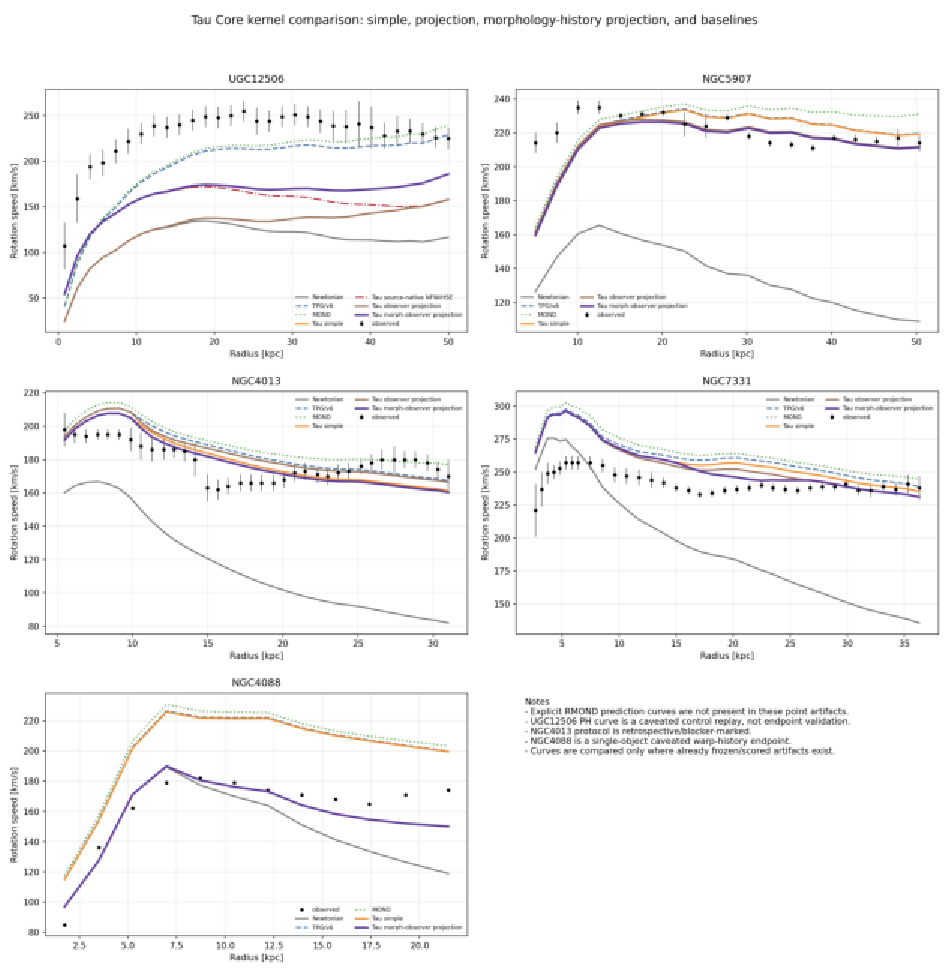
\includegraphics[width=\linewidth]{figures/fig20_projection_enriched_kernel_rotation_comparison.pdf}
\caption{Projection-enriched rotation-curve comparison for the five inspected
candidates.  The plotted curves show the measured rotation curve, Newtonian
baryonic comparator, TPG/v6 predecessor comparator, MOND comparator where
available in the point artifacts, the simple Tau morphology proxy, and the
observer/projection or morphology-trajectory enriched Tau variants.  An explicit
RMOND prediction curve is not present in the current point artifacts and is
therefore not drawn.  The figure is intended as kernel-development evidence: it
illustrates how the enriched kernel differs from the simpler morphology-only
proxy and from listed comparators.  It is not a population endpoint figure.}
\label{fig:projection-enriched-comparison}
\end{figure}

The audit is consistent with the expectation that observer/projection and
morphology-trajectory information is not a negligible correction to
morphology-specific readout kernels.  UGC12506 is the clearest stress case: the
simple envelope and observer-projection shells remain weak, the source-native
NFW/HSE shell improves the result, and the incremental projection-history shell
improves further, but the object still does not reach the strongest MOND/TPG
diagnostic curves.  This is evidence that projection-history matters, not an
endpoint success.  In NGC5907 this is natural because the system is edge-on and
projection-dominated.  In NGC4013, warp and vertical overlay make a mixed
readout plausible.  In NGC7331, the improvement is smaller and caveated by
outer-warp source-freeze choices.  In NGC4088, the improvement is large, but
the case is also the most source-review-sensitive because asymmetric history
and normalization choices matter.

\section{Time/projection diagnostic layers}
\label{sec:time-diagnostics}

\subsection{Full-time morphology phase diagnostic}

The preceding comparison uses the strongest available projection-enriched or
trajectory-enriched curve already present in the object-specific artifacts.  As
a separate diagnostic, we also ran a small ``full-time morphology'' phase layer
on the trial galaxies for which point-level projection artifacts are available.
In Tau Core language this is not a backward-causality term.  It is a
trajectory/phase component of the deeper morphology configuration, whose
four-dimensional present, past, and future appearances may be different readout
slices.  Operationally, the trial layer has the form
\begin{equation}
  v_{\rm FT}^2(R)
  =
  v_{\rm base}^2(R)
  +
  A_{\rm FT}({\rm source})\,K_{\rm FT}(R),
  \label{eq:full-time-trial}
\end{equation}
where \(v_{\rm base}\) is the already frozen morphology/projection curve,
\(K_{\rm FT}\) is a late-settling trajectory/phase kernel constructed from the
existing source-side projection kernel and radial support, and
\(A_{\rm FT}\) is fixed from the source-status load and the existing carrier
scale.  The observed rotation curve is used only for scoring.  The trial is not
an endpoint validation and is not a final path-aware kernel.  It is also not a
complete time-projection endpoint in the sense of
Eq.~\eqref{eq:time-readout-shell}; it is a first diagnostic proxy for the
possibility that projection-selected morphology phase and clock/readout phase
modify the inferred rotation together.

\begin{table}[H]
\centering
\small
\setlength{\tabcolsep}{4pt}
\begin{tabularx}{\linewidth}{@{}lrrrX@{}}
\toprule
Galaxy & Base & Full-time & Difference & Interpretation \\
\midrule
NGC4013 & 11.45 & 11.51 & \(+0.06\) &
slight degradation; existing warp/vertical-overlay curve is already close to
the accepted shape, so the added phase layer over-counts source structure
already carried by the mixed kernel \\
NGC4088 & 11.62 & 9.39 & \(-2.23\) &
clear improvement in the strongest warp/history/asymmetry case \\
NGC4183 & 6.25 & 6.25 & \(-0.00\) &
null-like response, as expected for a weak-projection control case \\
NGC5907 & 15.50 & 15.50 & \(-0.00\) &
nearly saturated projection kernel; the phase layer is effectively neutral \\
NGC7331 & 22.26 & 22.28 & \(+0.02\) &
slight degradation; broad mixed/outer-warp kernel may already include the
available phase information, so the phase proxy adds a diffuse correction
rather than a sharper independent source component \\
\bottomrule
\end{tabularx}
\caption{Diagnostic full-time morphology phase replay on trial galaxies.  RMSE
values are in km\,s\(^{-1}\).  Negative differences mean that the full-time
phase layer improved the existing source-frozen morphology/projection curve.
The construction is source-frozen and diagnostic only; no endpoint validation
claim is made.}
\label{tab:full-time-phase-diagnostic}
\end{table}

\begin{figure}[H]
\centering
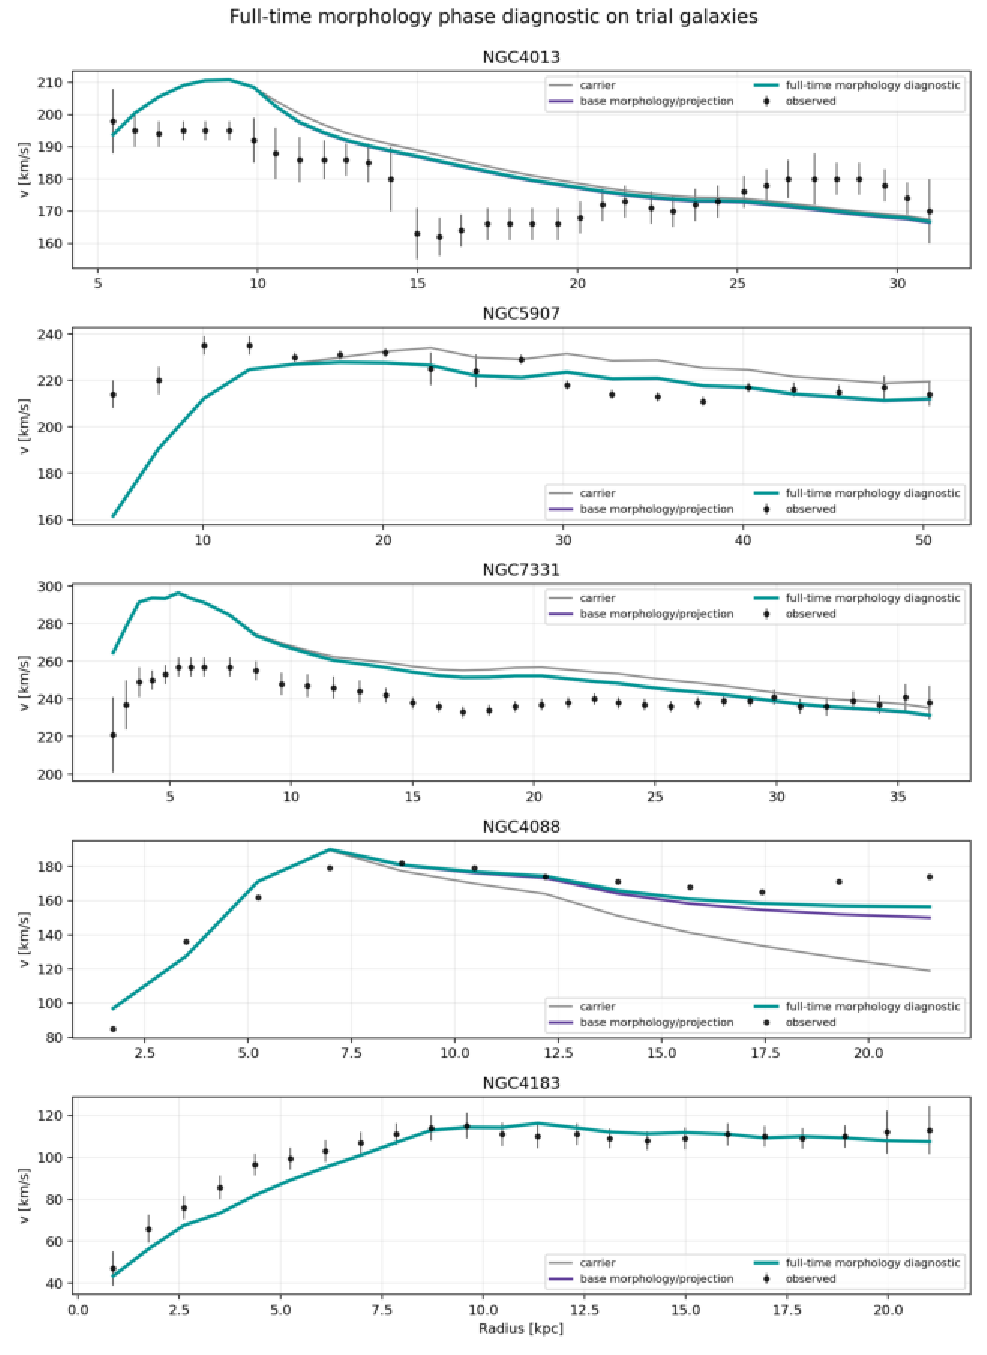
\includegraphics[width=\linewidth,height=0.68\textheight,keepaspectratio]{figures/fig21_full_time_morphology_trial_galaxy_rotation_curves.pdf}
\caption{Full-time morphology phase diagnostic on the trial galaxies.  The
purple curve is the already frozen morphology/projection baseline and the teal
curve adds the diagnostic trajectory/phase layer of
Eq.~\eqref{eq:full-time-trial}.  The layer gives a meaningful improvement only
for NGC4088, the strongest warp/history/asymmetry object in the current trial
set.  It is nearly neutral for NGC5907 and NGC4183 and slightly worsens NGC4013
and NGC7331.  This pattern is useful because the phase layer does not behave as
a universal gain knob; its effect is morphology/history dependent.}
\label{fig:full-time-phase-diagnostic}
\end{figure}

The diagnostic result is therefore claim-safe but informative.  The full-time
morphology phase layer is not a universal additive correction that improves
every galaxy by construction.  It helps most where the source status indicates
strong time/trajectory, warp, or asymmetry content, as in NGC4088.  In more
stable systems, or in systems where the projection/mixed kernel is already
close to saturated, the additional layer is negligible or slightly harmful.
This is consistent with the Tau Core expectation that trajectory/phase
information should be readout-relevant only for the morphology classes that
carry such information.

\subsection{Diagnostic \(\Xi_t\) replay}

To separate the additive morphology-phase proxy from the explicit clock/readout
shell of Eq.~\eqref{eq:time-readout-shell}, we ran one additional diagnostic.
The replay applies a small residual-blind factor
\(\Xi_t(R)=1+\epsilon_0 K_t(R)\) to the existing base and full-time curves.
The coefficient \(\epsilon_0\) is capped and derived from the same
source-status load used by the trajectory/phase replay.  It is not fitted from
the rotation residual.  This test asks only whether the time-readout direction
is plausible enough to motivate a future accepted \(\Xi_t(R)\) manifest.

\begin{table}[H]
\centering
\small
\setlength{\tabcolsep}{3pt}
\begin{tabularx}{\linewidth}{@{}lrrrrX@{}}
\toprule
Galaxy & Base & Additive & \(\Xi_t\)+base & \(\Xi_t\)+add. & Interpretation \\
\midrule
NGC4013 & 11.45 & 11.51 & 11.95 & 12.04 &
clock factor worsens an already good mixed/overlay curve; current clock proxy
is not independent of the active warp/vertical-overlay source context \\
NGC4088 & 11.62 & 9.39 & 10.50 & 8.38 &
clear improvement in strong warp/history/asymmetry case \\
NGC4183 & 6.25 & 6.25 & 6.24 & 6.24 &
nearly null response, consistent with weak-projection control status \\
NGC5907 & 15.50 & 15.50 & 15.52 & 15.53 &
slight degradation; projection kernel appears saturated \\
NGC7331 & 22.26 & 22.28 & 22.41 & 22.44 &
slight degradation; broad mixed outer-warp curve already carries the signal,
so the clock factor over-rescales a saturated broad-window proxy \\
UGC12506 & 69.18 & 64.12 & 67.90 & 62.97 &
improves the problematic high-spin edge-on stress case, but remains diagnostic \\
\bottomrule
\end{tabularx}
\caption{Diagnostic \(\Xi_t\) replay on trial galaxies.  Values are RMSE in
km\,s\(^{-1}\).  ``Additive'' is the full-time morphology phase proxy of
Eq.~\eqref{eq:full-time-trial}; the last two columns multiply the base or
additive curve by the small source-frozen clock/readout factor.  The replay is
not an accepted endpoint because no residual-blind \(\Xi_t(R)\) manifest has
yet been promoted.}
\label{tab:xi-time-diagnostic}
\end{table}

\begin{figure}[H]
\centering
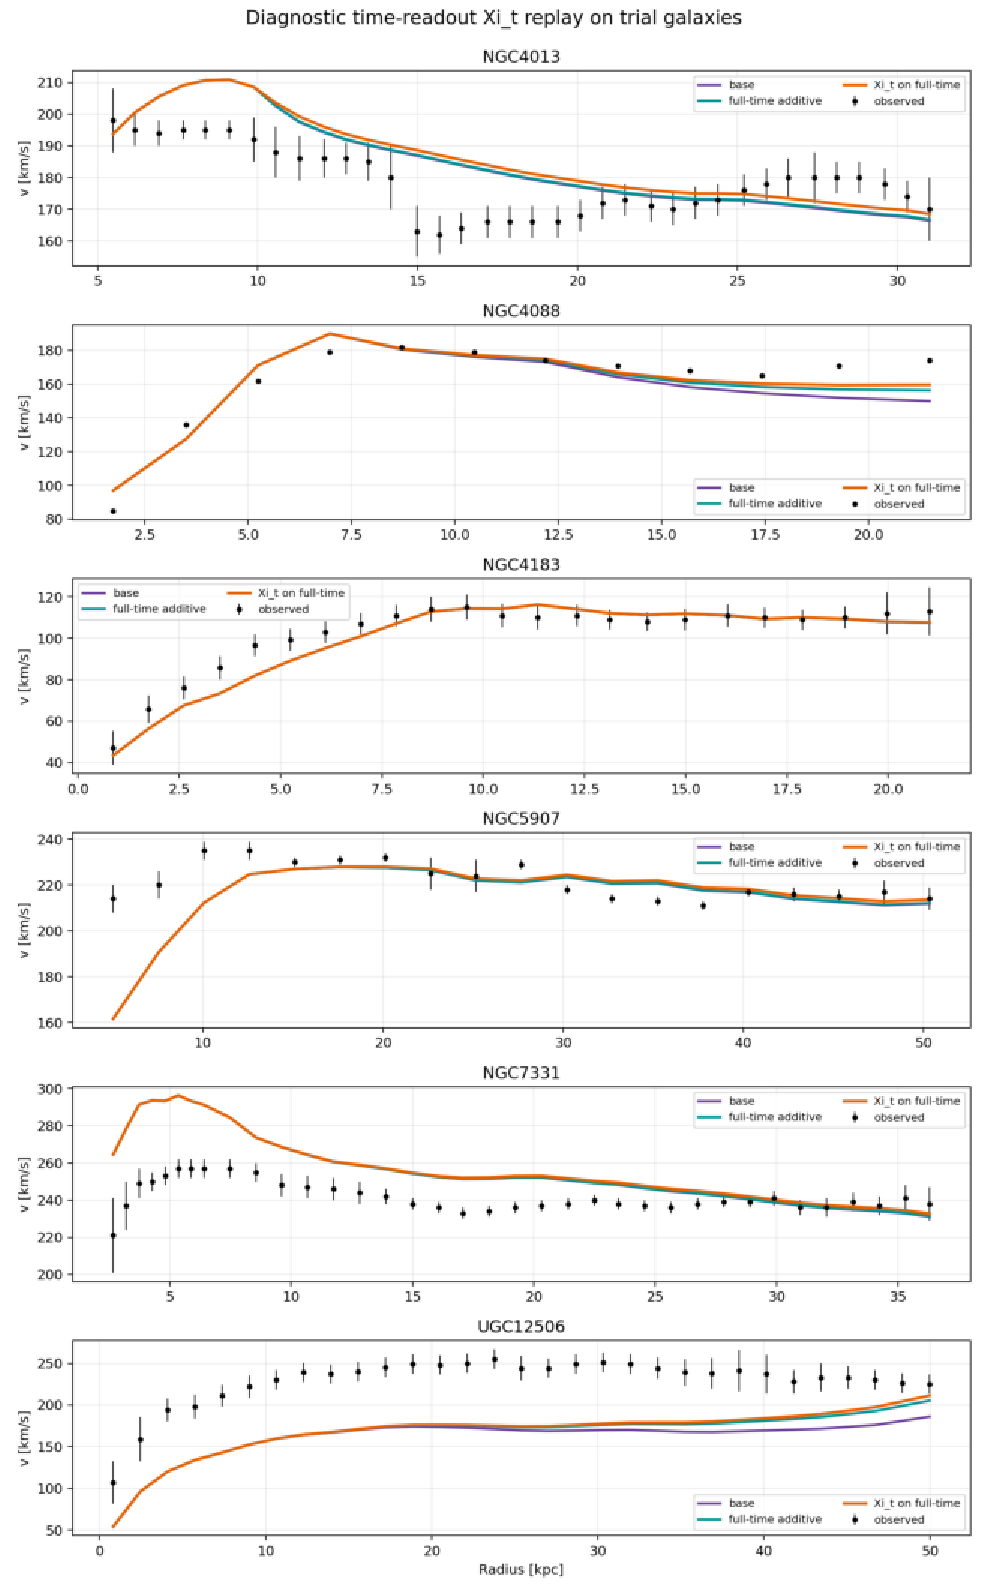
\includegraphics[width=\linewidth,height=0.72\textheight,keepaspectratio]{figures/fig22_time_readout_xi_trial_galaxy_rotation_curves.pdf}
\caption{Diagnostic \(\Xi_t\) replay.  The orange curve applies the small
time-readout factor to the full-time morphology proxy.  The effect improves
NGC4088 and UGC12506, is effectively neutral in NGC4183, and worsens the
already close NGC4013, NGC5907, and NGC7331 curves.  This non-universal pattern
is important: the time-readout factor is not acting as a generic amplitude
rescue.}
\label{fig:xi-time-diagnostic}
\end{figure}

The \(\Xi_t\) diagnostic strengthens the claim boundary rather than weakening
it.  If the clock/readout factor were merely a hidden curve-fitting knob, it
would be expected to improve all trial galaxies once turned on.  Instead, it
helps the two strongest stress cases in this sample: NGC4088, where
warp/history/asymmetry is explicit, and UGC12506, where high-spin edge-on
projection-history remains underpredicted.  It is neutral or harmful for more
regular or already saturated projection kernels.  This is only diagnostic
evidence, but it is consistent with the intended Tau Core interpretation: a
time-readout term should be morphology/path-state dependent, not universal.

The replay was therefore converted into manifest-readiness and double-count
audits rather than an endpoint claim, using the source-token priority protocol
of Subsection~\ref{subsec:source-token-priority}.  NGC4183 remains a weak/null control.
NGC4013, NGC5907, and NGC7331 reject or fail to support the current
\(\Xi_t\) proxy.  The failure modes are instructive rather than generic
negative results.  NGC4013 worsens because the existing mixed
warp/vertical-overlay kernel already encodes the source structure that the
generic clock proxy tries to rescale; the added factor therefore double-counts
the same geometry and moves an already close curve in the wrong direction.
NGC7331 worsens more mildly because the active vertical/outer-warp readout is
a broad-window proxy: the available phase information is already smeared into
the mixed kernel, so the clock factor over-rescales a saturated component
instead of adding a separately frozen clock/readout channel.  NGC5907 is
effectively neutral to slightly worse, consistent with an edge-on projection
kernel that is already saturated at the present proxy level.  Thus the
priority protocol must allow \(\Xi_t=1\) when no independent clock/readout evidence
exists; a degraded replay is a rejection of the current clock proxy, not a
post-hoc invitation to retune it from the residual.

NGC4088 is the clearest example of this discipline.  The clock-only replay
improves the base projection curve, and the additive-plus-clock stress curve is
numerically better than the accepted additive curve.  However, a source-space
overlap audit shows that the current \(\Xi_t\) ingredients---orientation
mismatch, onset-side radial support, warp strength, and morphology-history
phase---are already used by the additive warp/history kernel.  The accepted
combined route is therefore not the lower-RMSE additive-plus-clock stress
curve.  It is the caveated accepted additive warp/history endpoint with
\(\Xi_{\rm eff}=1\), RMSE \(=11.62\) km\,s\(^{-1}\).  The clock-only replay is
preserved as a control; reopening a time-projection endpoint for NGC4088 would
require new residual-blind clock/readout evidence that is demonstrably
non-overlapping with the active additive morphology kernel under the
\(T/A\) source-token priority test.

\section{UGC12506 stress case: channel separation and source-derived closure}
\label{sec:ugc12506-stress}

UGC12506 is kept separate from the general candidate audit because it plays a
different role.  It is the main stress case where the simpler projection and
time/projection controls move in the right direction but still leave a large
deficit.  This section therefore records the source-review gates, the
channel-separation ledger, and the source-derived closure candidate without
promoting the galaxy to an endpoint success.
UGC12506 is not used as a validation case in this manuscript.  It is a
stress-test and hypothesis-generation case: its role is to reveal which
additional source-side readout channels would have to be frozen and transferred
to independent galaxies before they can count as evidence.

\subsection{\(\Xi_t\) source-review route}

UGC12506 remains the active \(P1\) source-review target for a future accepted
\(\Xi_t(R)\) manifest.  It has strong high-inclination, extended-H~I,
asymmetric-envelope, low-density, and high-spin source context from the
HIghMass VLA route.  However, the foreground/path object term is not
established, so the current source-only policy is to set that path term to zero
unless a later cone or path-environment review supports it.  Its remaining open
step is a residual-blind high-spin/envelope clock proxy, not a foreground-rescue
term.

As a first UGC12506 shell, the source-only clock proxy can be written
\[
  \Xi_t(R)=1+\epsilon_t K_t(R),
\]
where \(K_t\) is assembled from high-spin settling, edge-on
position--velocity clock-slice, diffuse H~I envelope settling, and the
caveated approaching/receding asymmetry component, while the path-environment
component is set to zero.  The current source-shell artifact gives
\(\epsilon_t\simeq0.024\) from a bounded source-load rule.  This is not an
accepted endpoint: the remaining blocker is the accepted origin of the
\(\epsilon_t\) normalization law.
The bounded shape of that rule is now itself separated from the open scale:
given a nonnegative source load \(L\), the minimal dimensionless, monotone,
null-recovering, saturating response map is
\[
  \epsilon_t=\epsilon_{\rm cap}\frac{L}{1+L}.
\]
For UGC12506 the present source load gives \(L\simeq2.14\), hence
\(L/(1+L)\simeq0.68\).  The open part is not this bounded shape, but the
Tau-side or class-level origin of the small cap \(\epsilon_{\rm cap}\).
For the present source-shell replay we therefore freeze
\(\epsilon_{\rm cap}=0.035\) only as a conservative small-mismatch protocol
cap, not as a universal Tau Core constant.  The cap is chosen inside the
linearized time-readout regime: for \(\Xi_t=1+\epsilon_t\),
\(\Xi_t^2=1+2\epsilon_t+\epsilon_t^2\), so the neglected quadratic correction is
\(\epsilon_t/2\) of the linear term.  Requiring this ratio to be at most \(2\%\)
gives \(\epsilon_t\leq0.04\); the frozen cap \(0.035\) is below that bound, with
a maximum quadratic-to-linear ratio \(0.0175\) and a maximum squared-velocity
multiplier shift \((1.035)^2-1\simeq0.071\).  Thus the UGC12506 shell now has a
bounded source-load shape and a predeclared linear-regime cap, but it still does
not become an accepted endpoint until the cap policy is promoted by an
accepted-manifest or deeper Tau-side clock-geometry gate.
The current accepted-manifest gate therefore returns
\texttt{U12506\_XI\_T\_ACCEPTED\_MANIFEST\_NOT\_READY}: the shell passes the
no-residual-leakage, zero-path-policy, bounded-shape, and cap-protocol checks,
but remains blocked by the unreviewed \(K_t(R)\) envelope mapping and the
unfilled clock/readout settling proxy.  This is the intended protocol outcome:
UGC12506 is a strong source-shell target for a future \(\Xi_t\) endpoint, not an
endpoint result in this draft.
The corresponding source-review packet is now prepared with six review
obligations and five allowed responses.  It explicitly forbids using rotation
residuals, endpoint RMSE, baseline ranks, wrong-family Tau scores, post-hoc cap
changes, or foreground-rescue arguments to promote the route.  Its status is
\texttt{U12506\_XI\_T\_SOURCE\_REVIEW\_PACKET\_READY\_RESPONSE\_PENDING}; the
next action is an independent source response, not endpoint scoring.
The response-intake validator has also been exercised on a completed
residual-blind reviewer response.  The reviewer selected
\texttt{ACCEPT\_KT\_CARRY\_CAP\_AS\_CAVEATED\_INTERVAL}: the high-spin,
edge-on PV/envelope, and extended H~I support route may be carried forward as a
caveated interval/control manifest, while the asymmetry term remains a
caveated phase component, the path term remains zero, and
\(\epsilon_{\rm cap}=0.035\) remains a protocol cap rather than a universal Tau
Core constant.  The intake validator records the response as usable for the
manifest gate but still endpoint-blocked.  The accepted-manifest gate therefore
returns a caveated-interval/control-ready, endpoint-blocked status; the exact
machine-readable status is recorded in the released gate summary.
Finally, a reviewer handoff has been generated for this route.  It contains a
fillable response form, six source-review tasks, five allowed route-level
responses, forbidden-input guardrails, and input hashes.  This handoff is the
artifact to send to an external or otherwise separated residual-blind reviewer.
A portable handoff bundle is also generated at
\texttt{review\_bundles/ugc12506\_xi\_t\_external\_review\_bundle.zip}.  The
bundle contains the prompt, usage note, fillable response form, source-review
packet, source evidence tables, forbidden-input ledger, and a relative-path hash
manifest.  It is a review-handoff artifact only: a completed response must still
pass the intake validator and accepted-manifest gate before any endpoint score
is allowed.
The resulting caveated control manifest is stored in the released
\texttt{data/derived} artifact
\texttt{ugc12506\_xi\_t\_caveated\_interval\_control\_manifest.csv}.
It freezes \(\epsilon_t\in[0,0.0238438]\), \(\Xi_t\in[1,1.02384]\), and a
zero path term for any future control replay.  It does not authorize a standard
endpoint score.
Running that frozen manifest as a caveated control replay gives a small but
not decisive movement: the lower edge of the interval has RMSE \(77.54\)
km\,s\(^{-1}\), while the upper edge has RMSE \(76.49\) km\,s\(^{-1}\).  The
improvement is therefore about \(1.06\) km\,s\(^{-1}\), and no observed point is
contained inside the narrow \(\Xi_t\) interval, even allowing measurement
errors.  This is scientifically useful precisely because it is not an
all-purpose rescue term: the source-reviewed cap moves the curve in the
expected direction but is too small to close the UGC12506 deficit by itself.
Thus UGC12506 remains a caveated control case, not a positive endpoint.

\subsection{\(\Theta_{\rm morph}\) and \(\Xi_t\) channel separation}

With the refined Tau morphology-state terminology, the UGC12506
\(\Theta_{\rm morph}\) and \(\Xi_t\) routes can now be separated cleanly.  The
\(\Theta_{\rm morph}\) replay has the additive form
\[
  v_\theta^2(R)=v_{\rm projection/history}^2(R)+A_\theta K_\theta(R),
\]
so it is a morphology-state phase or late-settling diagnostic.  The
\(\Xi_t\) route instead has the multiplicative interval-control form
\[
  \Xi_t(R)=1+\epsilon_t K_t(R),
\]
so it is a clock/readout control.  The released separation gate records a
``channels separated, endpoint still blocked'' status: the formula roles are
distinct, but the high-spin/envelope/asymmetry source context still partially
overlaps and the path term remains unestablished.
Consequently the separation is an architectural clarification and a control
ledger improvement, not an endpoint validation claim.
The follow-up source-nonoverlap gate sharpens this further.  It assigns the
late-settling outer radial shape to the \(\Theta_{\rm morph}\) channel and the
small-mismatch \(\epsilon_t\) cap to the \(\Xi_t\) channel, but keeps high spin,
the extended low-density H~I envelope, edge-on position--velocity geometry,
and approaching/receding H~I asymmetry as shared or partially shared context.
The gate therefore returns a partial-nonoverlap status: a combined-control
replay is allowed with those assignments frozen, but a combined endpoint
remains blocked until non-overlapping clock/path evidence is supplied.
Running that ledger-frozen combined-control replay gives a useful but still
non-endpoint result.  The \(\Theta_{\rm morph}\)-only diagnostic has RMSE
\(64.12\) km\,s\(^{-1}\).  The ledger-strict combined control, which uses the
\(\Theta_{\rm morph}\) late-settling shape plus only the \(\Xi_t\)
small-mismatch cap, improves this to \(60.31\) km\,s\(^{-1}\).  By contrast,
the caveated shared-context \(K_t(R)\) stress curve reaches only
\(63.21\) km\,s\(^{-1}\).  This is the desired claim-safe behavior: the
cleaner ledger-separated control moves in the helpful direction, while the
shared-context route is preserved as a caveated stress test rather than being
used as an endpoint rescue.

\begin{figure}[H]
\centering
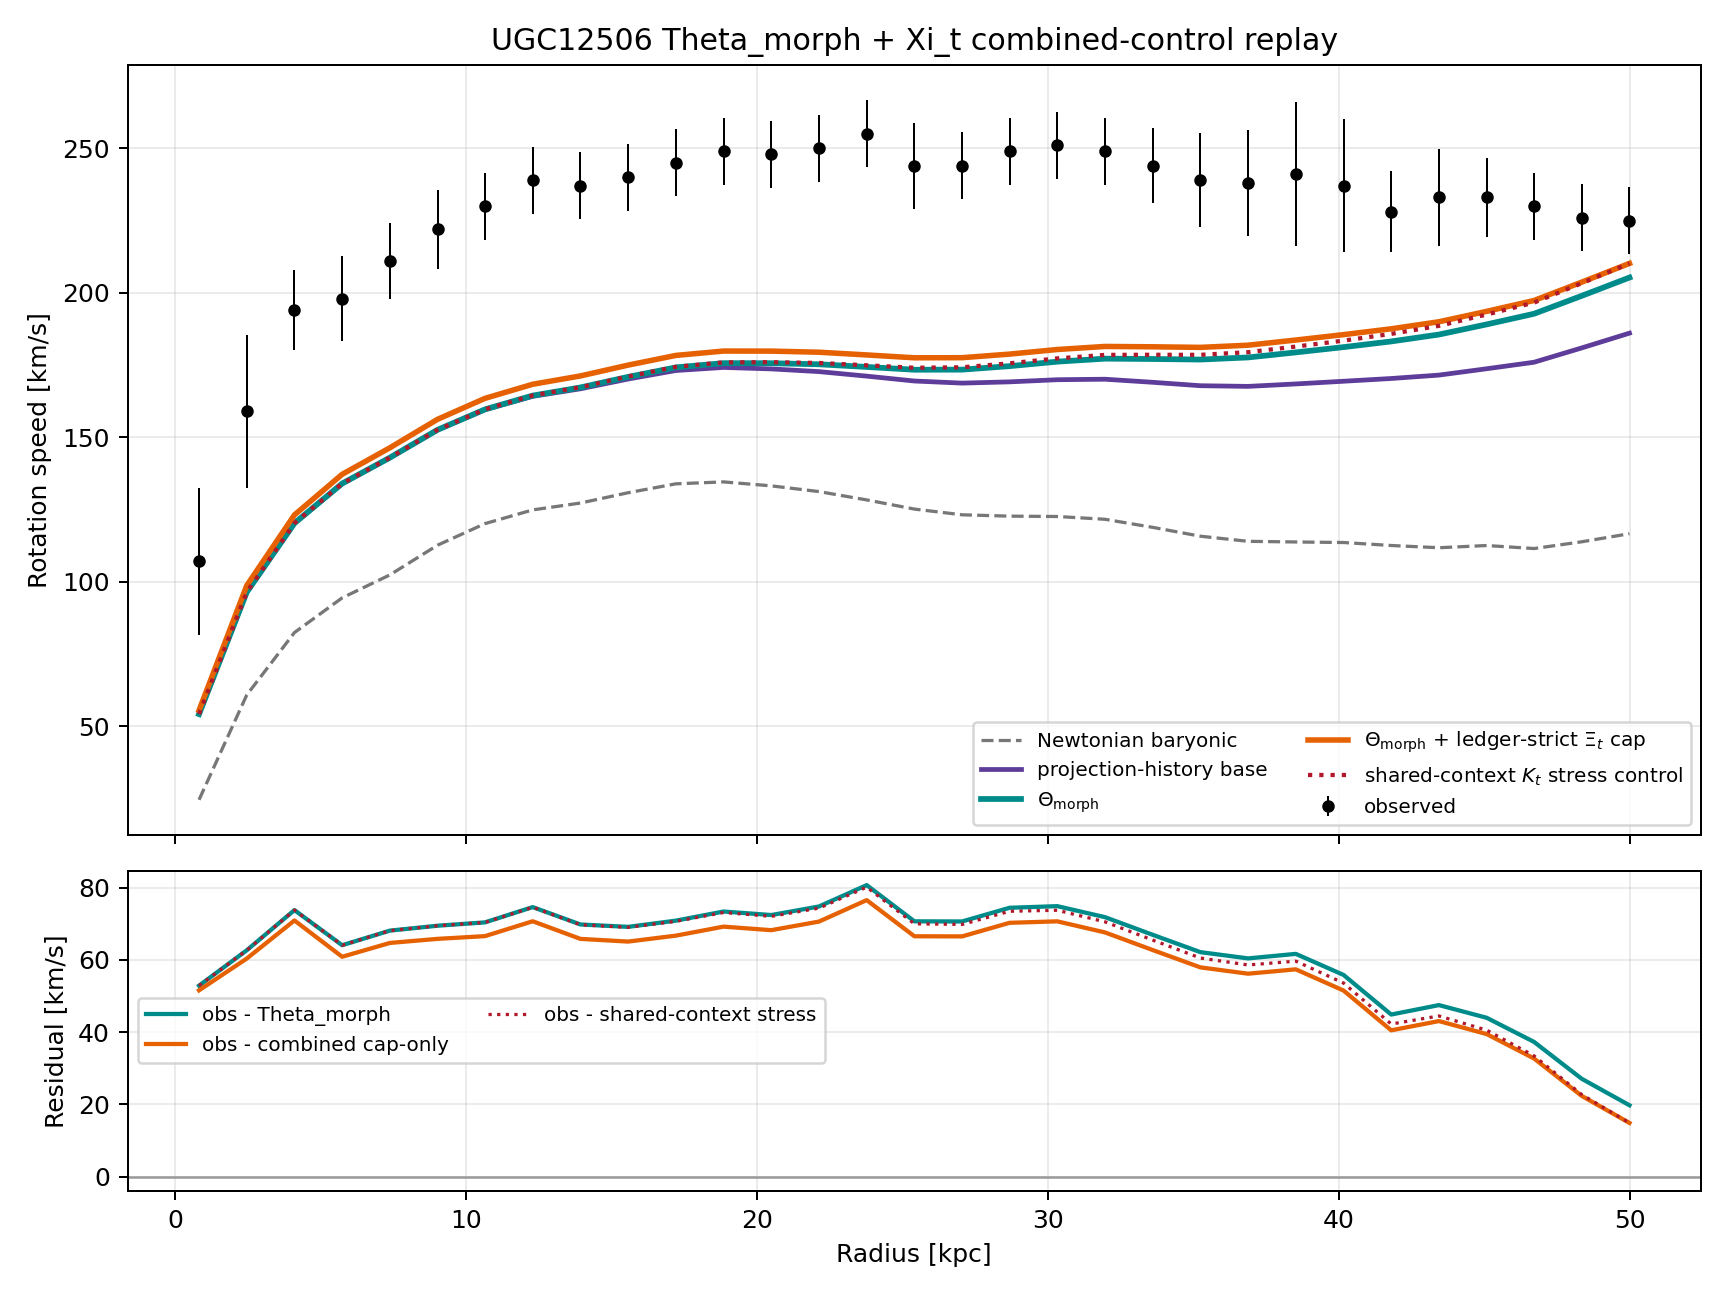
\includegraphics[width=\linewidth]{figures/fig25_ugc12506_theta_xit_combined_control_replay.png}
\caption{UGC12506 \(\Theta_{\rm morph}+\Xi_t\) combined-control replay.  The
orange curve is the ledger-strict control: the additive \(\Theta_{\rm morph}\)
phase curve multiplied only by the \(\Xi_t\) protocol cap.  The dotted red
curve is the shared-context \(K_t(R)\) stress control and remains caveated
because its source evidence overlaps the morphology channel.  This figure is a
control replay, not endpoint validation.}
\label{fig:ugc12506-theta-xit-combined-control}
\end{figure}

Figure~\ref{fig:ugc12506-comparison-rotation-curves} shows the same result in
direct comparison with the Newtonian baryonic, source-native NFW-HSE, and
projection-history curves.  The residual panel is included to make clear that
the combined-control curve reduces the systematic underprediction but does not
close the UGC12506 gap.  The comparison is therefore evidence for channel
accounting and kernel development, not a population or endpoint validation.

\begin{figure}[H]
\centering
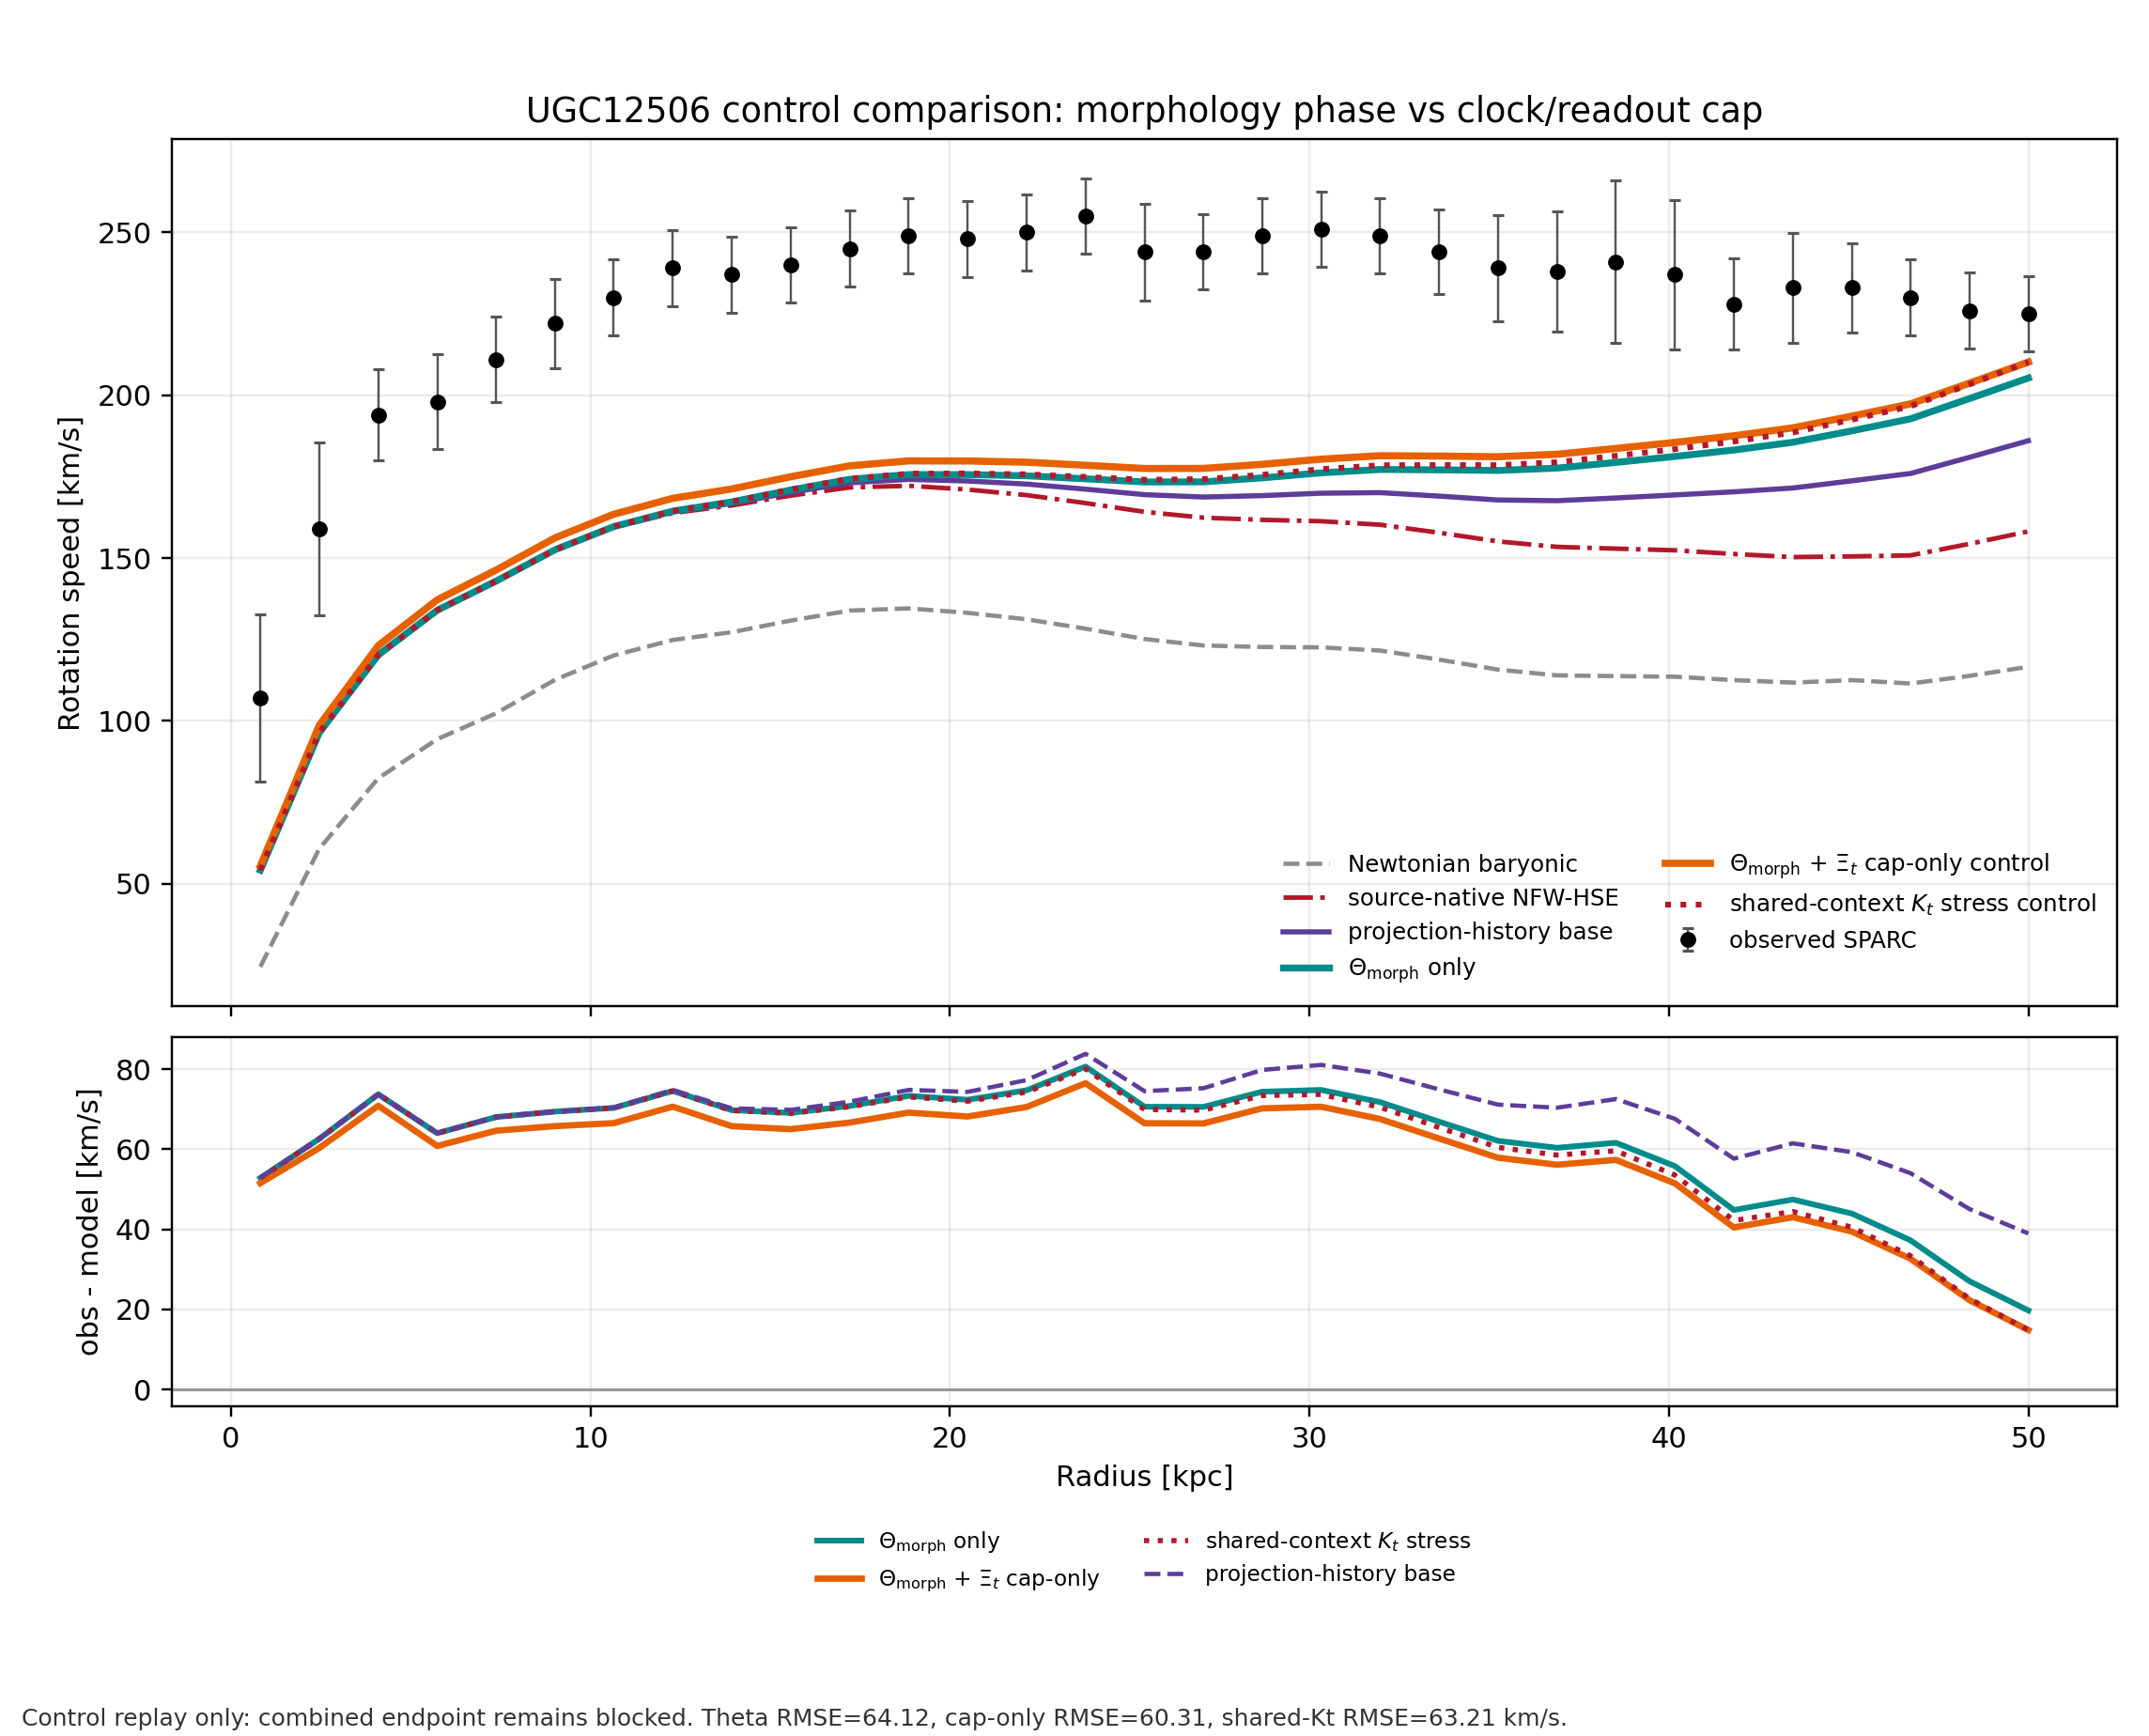
\includegraphics[width=\linewidth]{figures/fig26_ugc12506_comparison_rotation_curves.png}
\caption{UGC12506 comparison rotation curves.  The ledger-strict
\(\Theta_{\rm morph}+\Xi_t\) cap-only control is the best current
source-ledger control in this comparison, but all displayed Tau Core curves
remain below the observed rotation curve over much of the disk.  The
shared-context \(K_t\) stress curve is shown separately to avoid hiding the
source-overlap caveat.}
\label{fig:ugc12506-comparison-rotation-curves}
\end{figure}

\section{Cross-galaxy controls for the time/projection layer}
\label{sec:time-control-audit}

\subsection{Control-galaxy audit of the current time/projection layer}

We also asked whether the same time/projection--morphology layer improves the
other inspected control galaxies.  This is again a diagnostic audit rather
than endpoint validation.  The answer is selective.  Relative to the
morphology-only proxy, the combined time/projection layer improves clearly for
UGC12506 (\(\Delta{\rm RMSE}=-3.81\) km\,s\(^{-1}\)) and NGC4088
(\(-1.04\) km\,s\(^{-1}\)), is nearly neutral for NGC4183
(\(-0.01\) km\,s\(^{-1}\)) and NGC5907 (\(+0.03\) km\,s\(^{-1}\)), and worsens
the current proxy for NGC7331 (\(+0.16\) km\,s\(^{-1}\)) and NGC4013
(\(+0.53\) km\,s\(^{-1}\)).  This behavior is important for the claim
boundary.  The time/projection layer is not acting as a universal amplitude
knob; it helps primarily in cases where the source context indicates strong
history, asymmetry, or projection-clock relevance.  Where it worsens, the
cause is not treated as a free refit opportunity.  In NGC4013 the current
time/projection factor overlaps the already active warp/vertical-overlay mixed
kernel, so it double-counts rather than supplies an independent clock/readout
channel.  In NGC7331 the vertical/outer-warp window is broad enough that the
mixed kernel already carries the available phase information; the extra factor
therefore over-rescales a saturated proxy.  These rows are retained as
negative-control evidence for the default rule \(\Xi_t=1\) unless independent,
non-overlapping clock/readout evidence is source-frozen before scoring.

\begin{figure}[H]
\centering
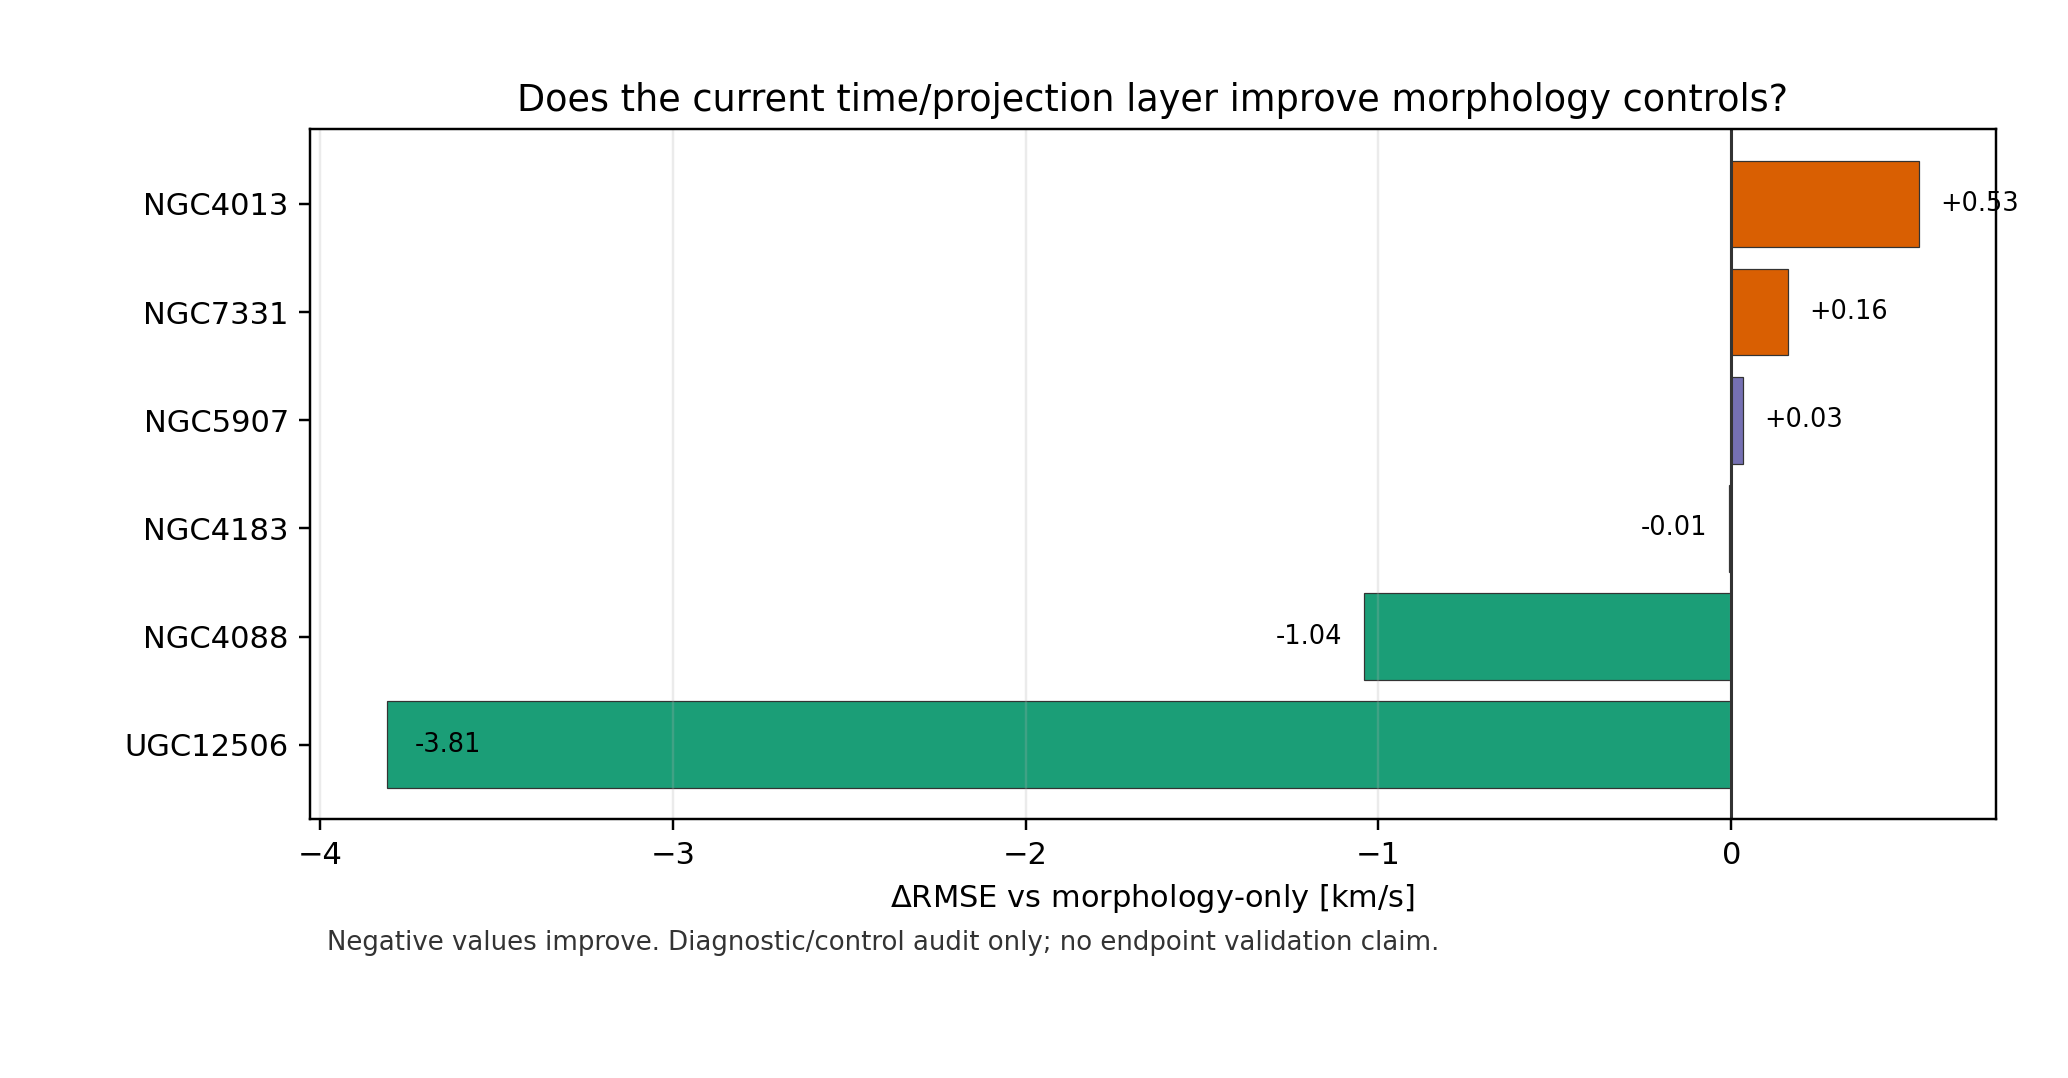
\includegraphics[width=\linewidth]{figures/fig27_time_morphology_control_improvement_audit.png}
\caption{Control-galaxy audit of the current time/projection--morphology
layer.  Negative values improve relative to the morphology-only proxy.  The
effect is selective: it improves clearly for UGC12506 and NGC4088, is nearly
neutral for NGC4183 and NGC5907, and worsens the current proxy for NGC7331 and
NGC4013.  This is a diagnostic/control audit, not endpoint validation.}
\label{fig:time-morphology-control-improvement}
\end{figure}

\subsection{Why the improving cases improve}

The two clearly improving rows in Fig.~\ref{fig:time-morphology-control-improvement}
are also the two rows for which the source-side morphology makes a
time/projection readout contribution most plausible.  This does not prove a
final Tau Core time-projection law, but it explains why the current diagnostic
layer improves these cases rather than behaving as a universal gain term.

For UGC12506, the source context is a high-inclination, high-spin system with
an extended H~I envelope and strong projection-history stress.  The simpler
Tau morphology and projection-history curves underpredict the measured
rotation over much of the disk.  The ledger-strict
\(\Theta_{\rm morph}+\Xi_t\) cap-only control improves the
\(\Theta_{\rm morph}\)-only diagnostic from \(64.12\) to
\(60.31\) km\,s\(^{-1}\).  The physical reading is that the late-settling
outer radial shape and the small clock/readout interval cap both move the
curve in the expected direction for an edge-on high-spin envelope system.  The
source-overlap ledger remains essential: the improvement is evidence for a
projection/time-relevant channel, not an accepted endpoint.

For NGC4088, the source context is qualitatively different.  The system is a
strong warp/history/asymmetry case, so the additional trajectory/phase layer is
expected to matter more than in regular disks.  The full-time morphology proxy
improves the base projection curve from \(11.62\) to \(9.39\) km\,s\(^{-1}\),
and the diagnostic \(\Xi_t\) replay reaches \(8.35\) km\,s\(^{-1}\).  The
interpretation is therefore not simply ``more amplitude''.  The added layer is
acting where the source morphology already indicates unsettled/asymmetric
readout structure.  Because the clock ingredients overlap the accepted
additive warp/history kernel, the lower-RMSE clock curve is still retained as
a control rather than promoted to the accepted endpoint route.

\begin{figure}[H]
\centering
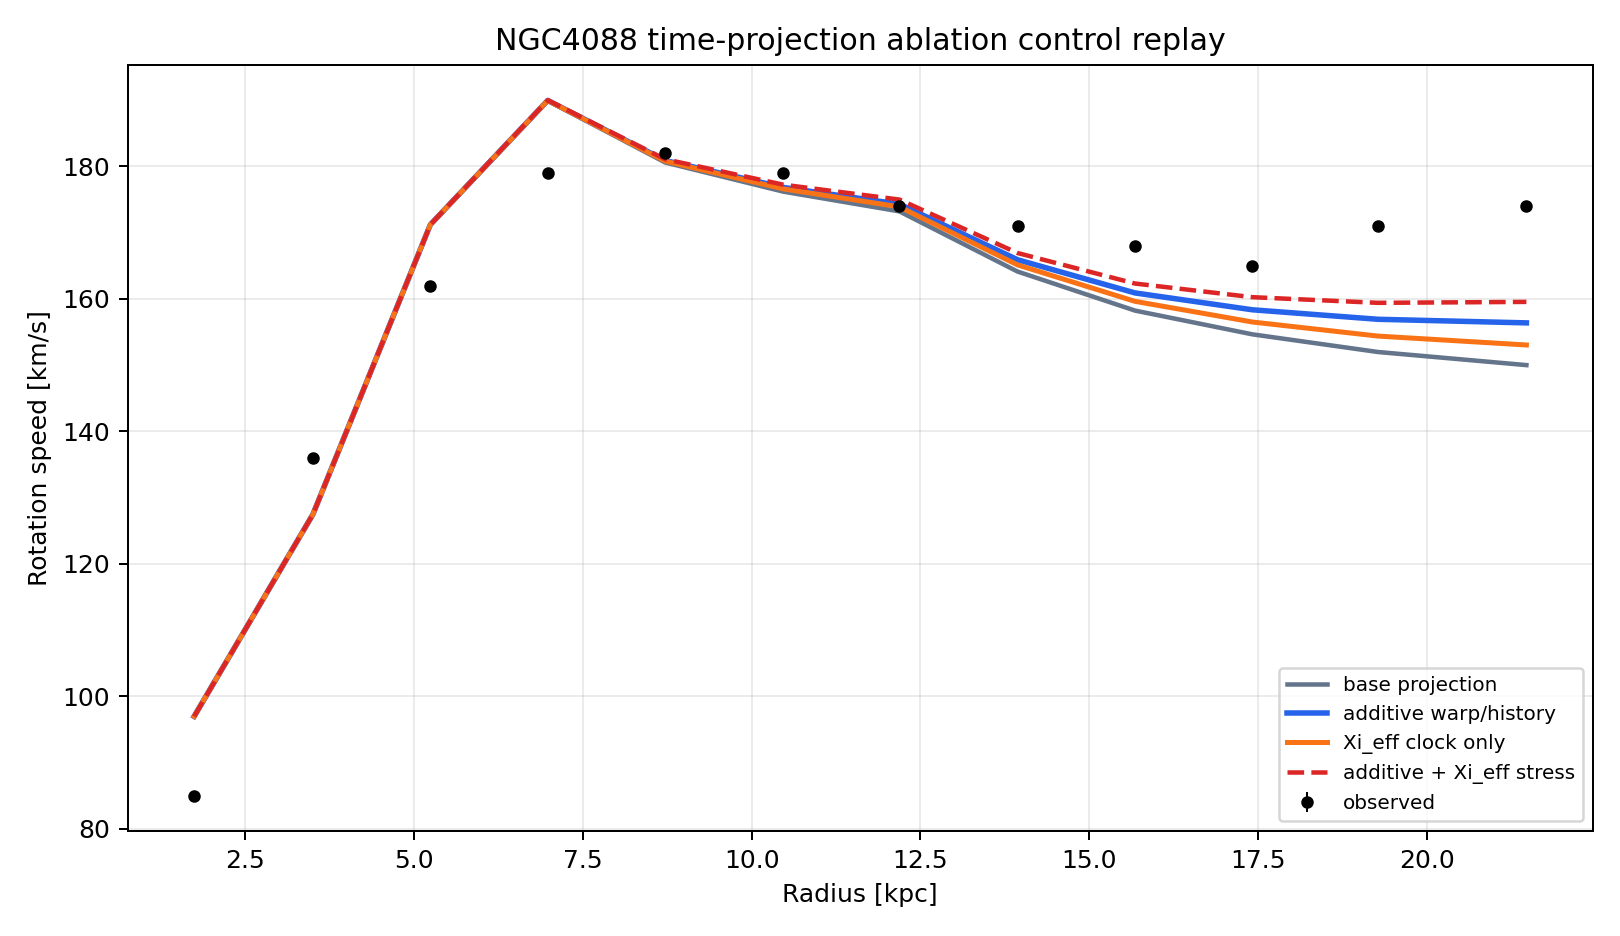
\includegraphics[width=\linewidth]{figures/fig28_ngc4088_time_projection_ablation_control_replay.png}
\caption{NGC4088 time/projection ablation control.  The improvement is largest
when the trajectory/phase proxy and the small \(\Xi_t\) replay are both active,
which is consistent with the source-side warp/history/asymmetry classification.
The figure is a control replay: it motivates the time/projection channel, but
does not promote a final clock endpoint because the clock evidence is not yet
independent of the accepted additive warp/history kernel.}
\label{fig:ngc4088-time-projection-ablation}
\end{figure}

\begin{figure}[H]
\centering
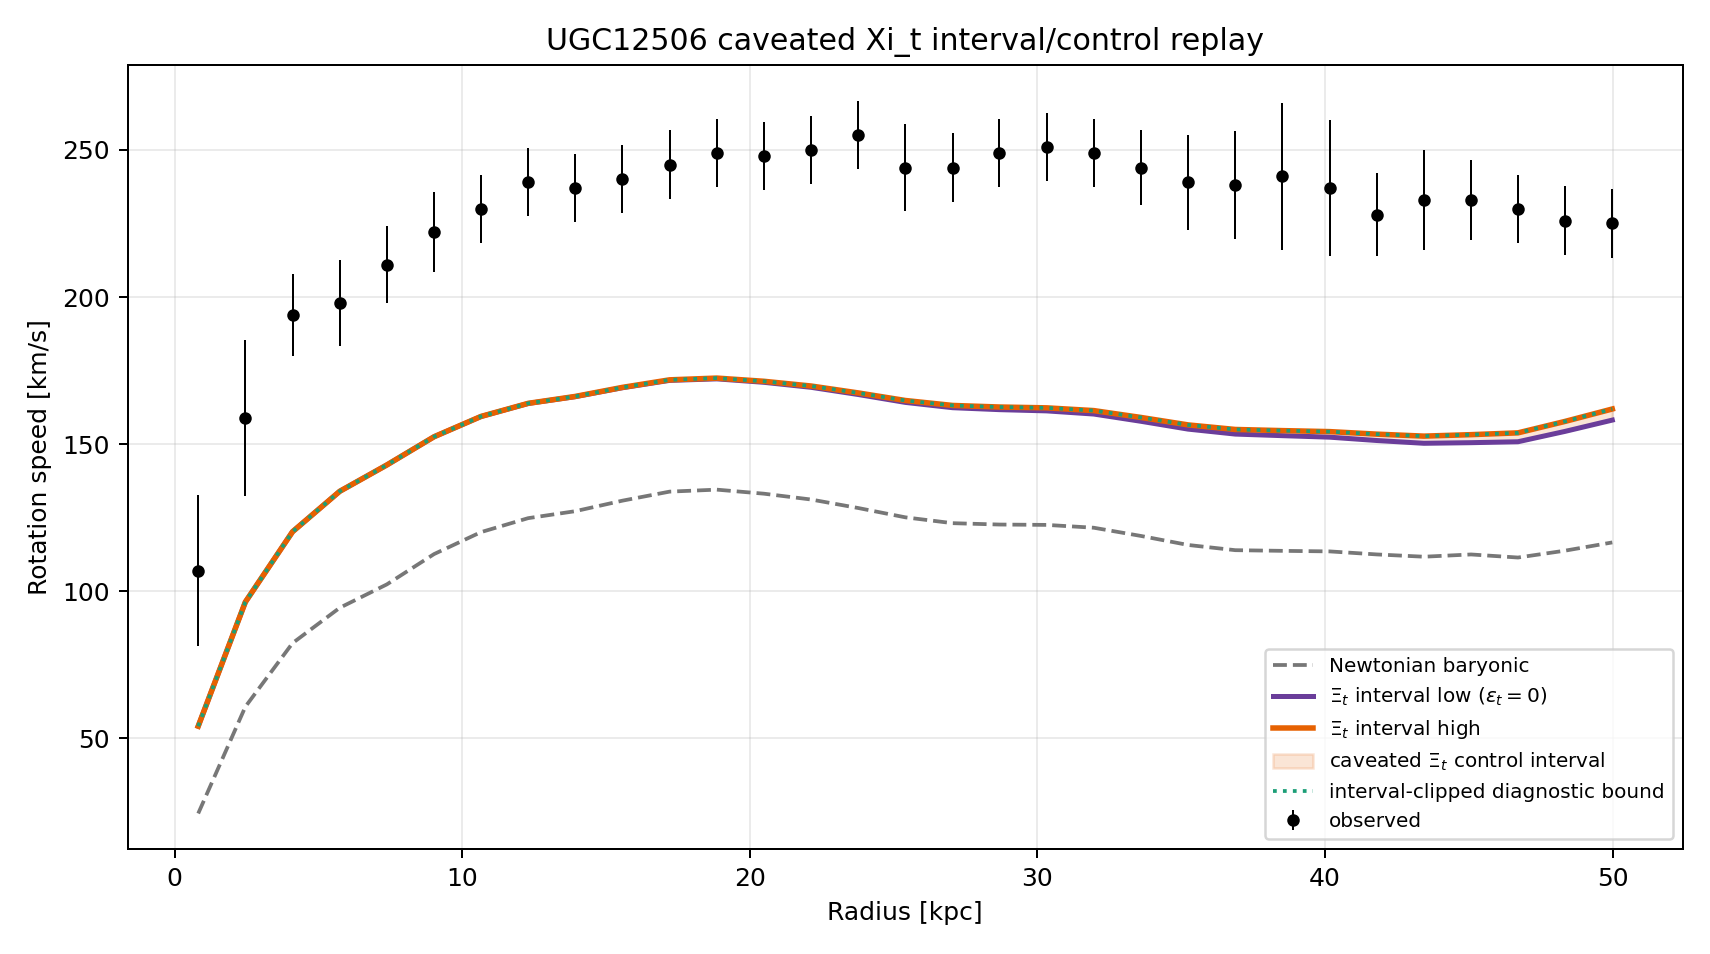
\includegraphics[width=\linewidth]{figures/fig23_ugc12506_xi_t_caveated_interval_control_replay.png}
\caption{UGC12506 caveated \(\Xi_t\) interval/control replay.  The shaded band
is the source-reviewed control interval allowed by the completed reviewer
response.  The interval improves the source-native base slightly but does not
contain the observed rotation curve.  The dotted clipped curve is a diagnostic
lower bound inside the frozen interval, not a fitted model.}
\label{fig:ugc12506-xit-control}
\end{figure}

\section{UGC12506 source-native mass/envelope--closure route}
\label{sec:ugc12506-closure}

\subsection{Source-native ablation and post-diagnostic beta closure}

The next-gate ledger identifies UGC12506 as the case where the remaining
deficit is least plausibly solved by a generic clock multiplier alone.  We
therefore ran the first source-native mass/envelope--closure ablation using
the published NFW/high-spin-envelope source route.  The kernel and amplitude
are frozen before scoring from source-side quantities; the observed rotation
curve enters only in the replay score.  The result improves the older
\(R_d\)-proxy NFW/HSE branch slightly, from \(77.86\) to
\(77.54\) km\,s\(^{-1}\) RMSE, and improves strongly over the pure
edge-on/envelope/asymmetry and source-envelope controls, both near
\(102.45\) km\,s\(^{-1}\).  It also improves over the baryonic carrier
(\(116.02\) km\,s\(^{-1}\)).  However, it remains far worse than the prior
diagnostic Tau/MOND/TPG-level references, whose best diagnostic RMSE is
\(37.36\) km\,s\(^{-1}\).  This is therefore useful source-side evidence for
a real mass/envelope--closure channel, not an endpoint validation and not a
closed UGC12506 solution.

\begin{figure}[H]
\centering
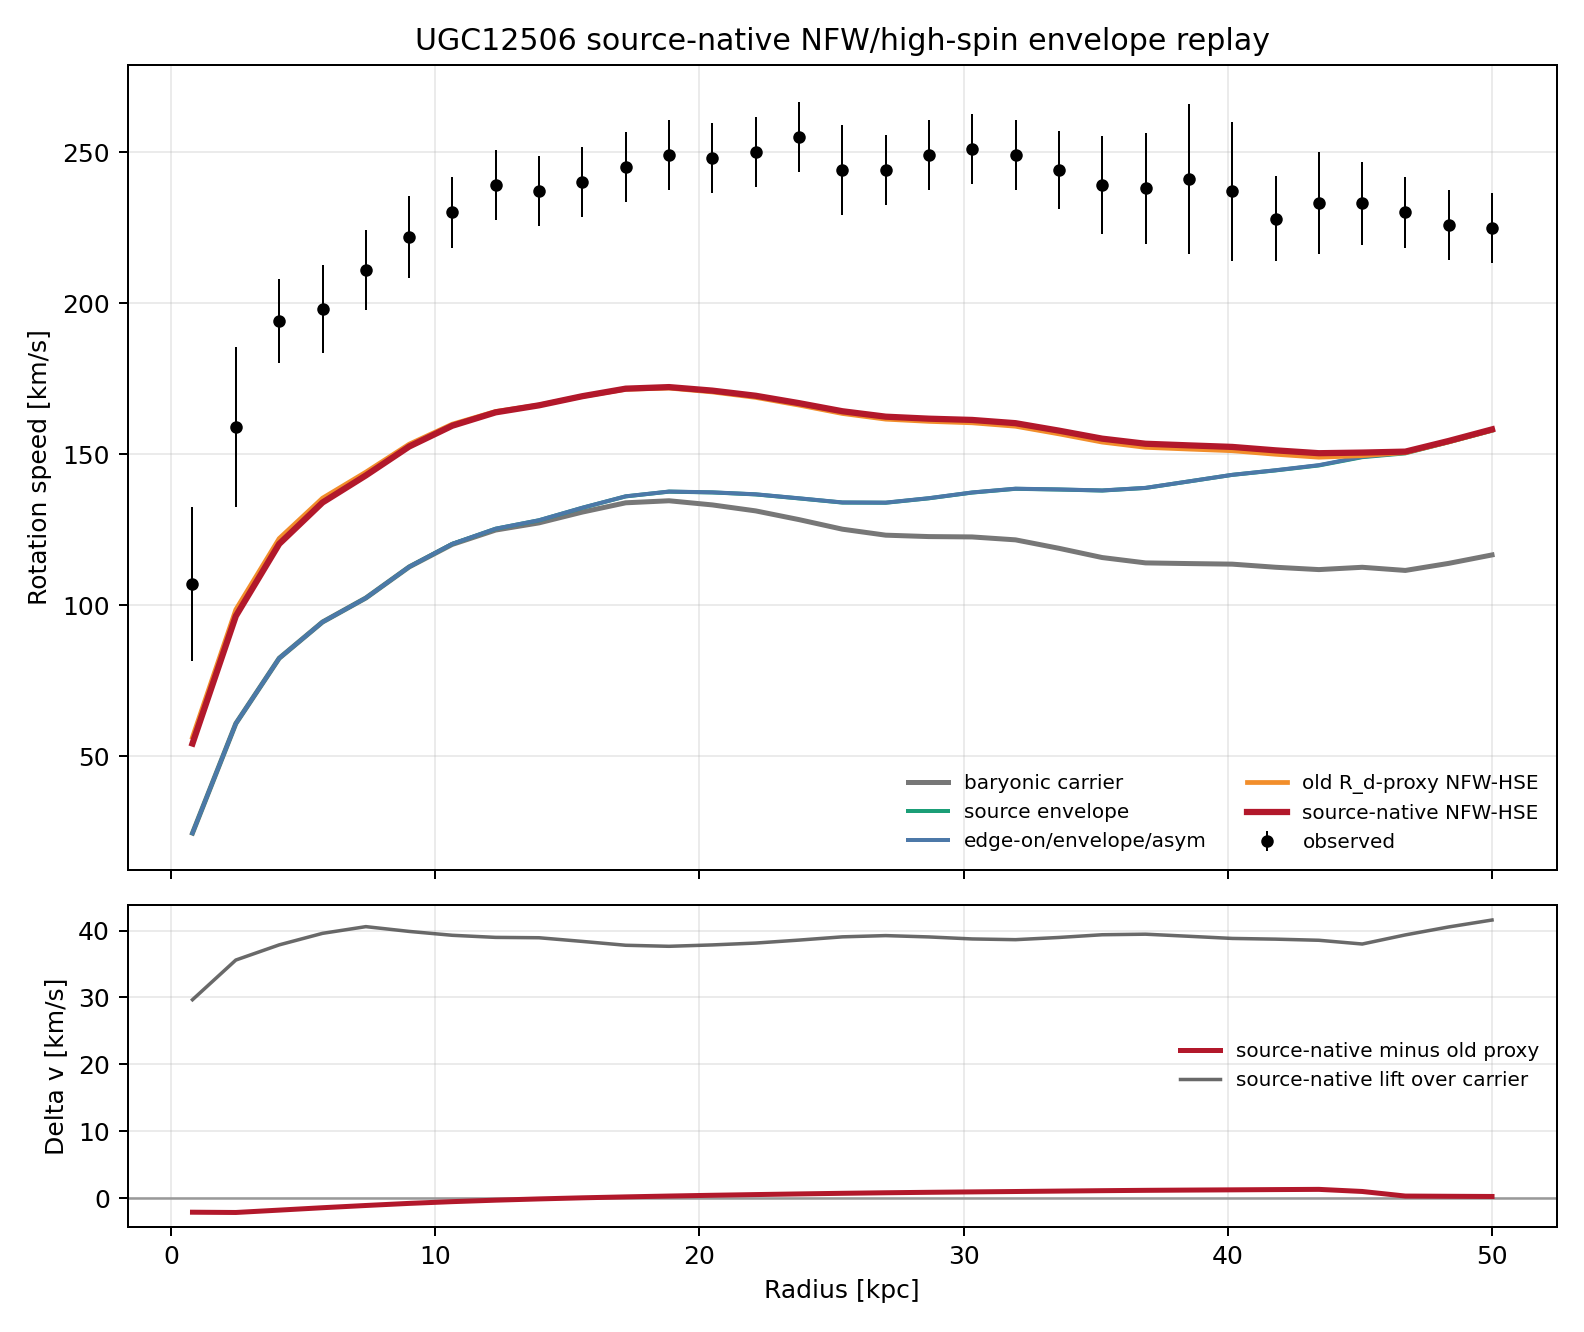
\includegraphics[width=\linewidth]{figures/fig29_ugc12506_source_native_nfw_hse_replay.png}
\caption{UGC12506 source-native NFW/high-spin-envelope replay.  The red curve
uses source-native NFW/HSE parameters and improves the older \(R_d\)-proxy
branch and lower source-envelope controls, but it still underpredicts the
observed curve substantially.  The replay is frozen before scoring and remains
a control result, not an endpoint validation.}
\label{fig:ugc12506-source-native-nfw-hse}
\end{figure}

The shape failure is therefore mostly an amplitude-normalization failure.  A
separate diagnostic fit keeps the NFW/HSE shape fixed and allows only one
velocity-squared amplitude multiplier.  The residual-aware optimum is
\(\beta_{\rm diag}=3.876\), which reduces the RMSE to \(7.48\) km\,s\(^{-1}\).
This diagnostic is not endpoint evidence, because \(\beta_{\rm diag}\) uses
the observed curve.  It is nevertheless useful: it says that the source-native
NFW/HSE shape is already close enough, and that the missing object is a
source-side normalization law.

A first source-only candidate for that normalization is
\[
\beta_{\rm cl}
= 1
  + {\lambda_{\rm spin}\over\lambda_{\rm ref}}
    \left({\chi^2_{\rm iso}\over\chi^2_{\rm NFW}}-1\right)_+
  + \sin^2 i\,\max\!\left({i-80^\circ\over 10^\circ},0\right),
\]
with \(\lambda_{\rm ref}=0.10\).  The terms are dimensionless: high spin
amplifies the source-native NFW closure preference, while the last term is the
edge-on projection load.  For UGC12506 this gives
\(\beta_{\rm cl}=3.954\), within \(2.1\%\) of the residual-aware diagnostic
normalization, and gives \(7.67\) km\,s\(^{-1}\) RMSE.  The calculation uses
only source-frozen spin, Table-5 halo preference, and inclination, but the
formula was written after the normalization diagnostic.  It is therefore a
post-diagnostic source-candidate replay, not a source-frozen endpoint law.  A
future paper-grade promotion would require predeclaring this \(\beta_{\rm cl}\)
rule and testing it on independent high-spin edge-on systems before endpoint
scoring.
This formula is not counted as evidence on UGC12506.  Its only admissible role
in the present paper is to define a frozen transfer hypothesis for independent
high-spin edge-on systems.

\begin{figure}[H]
\centering
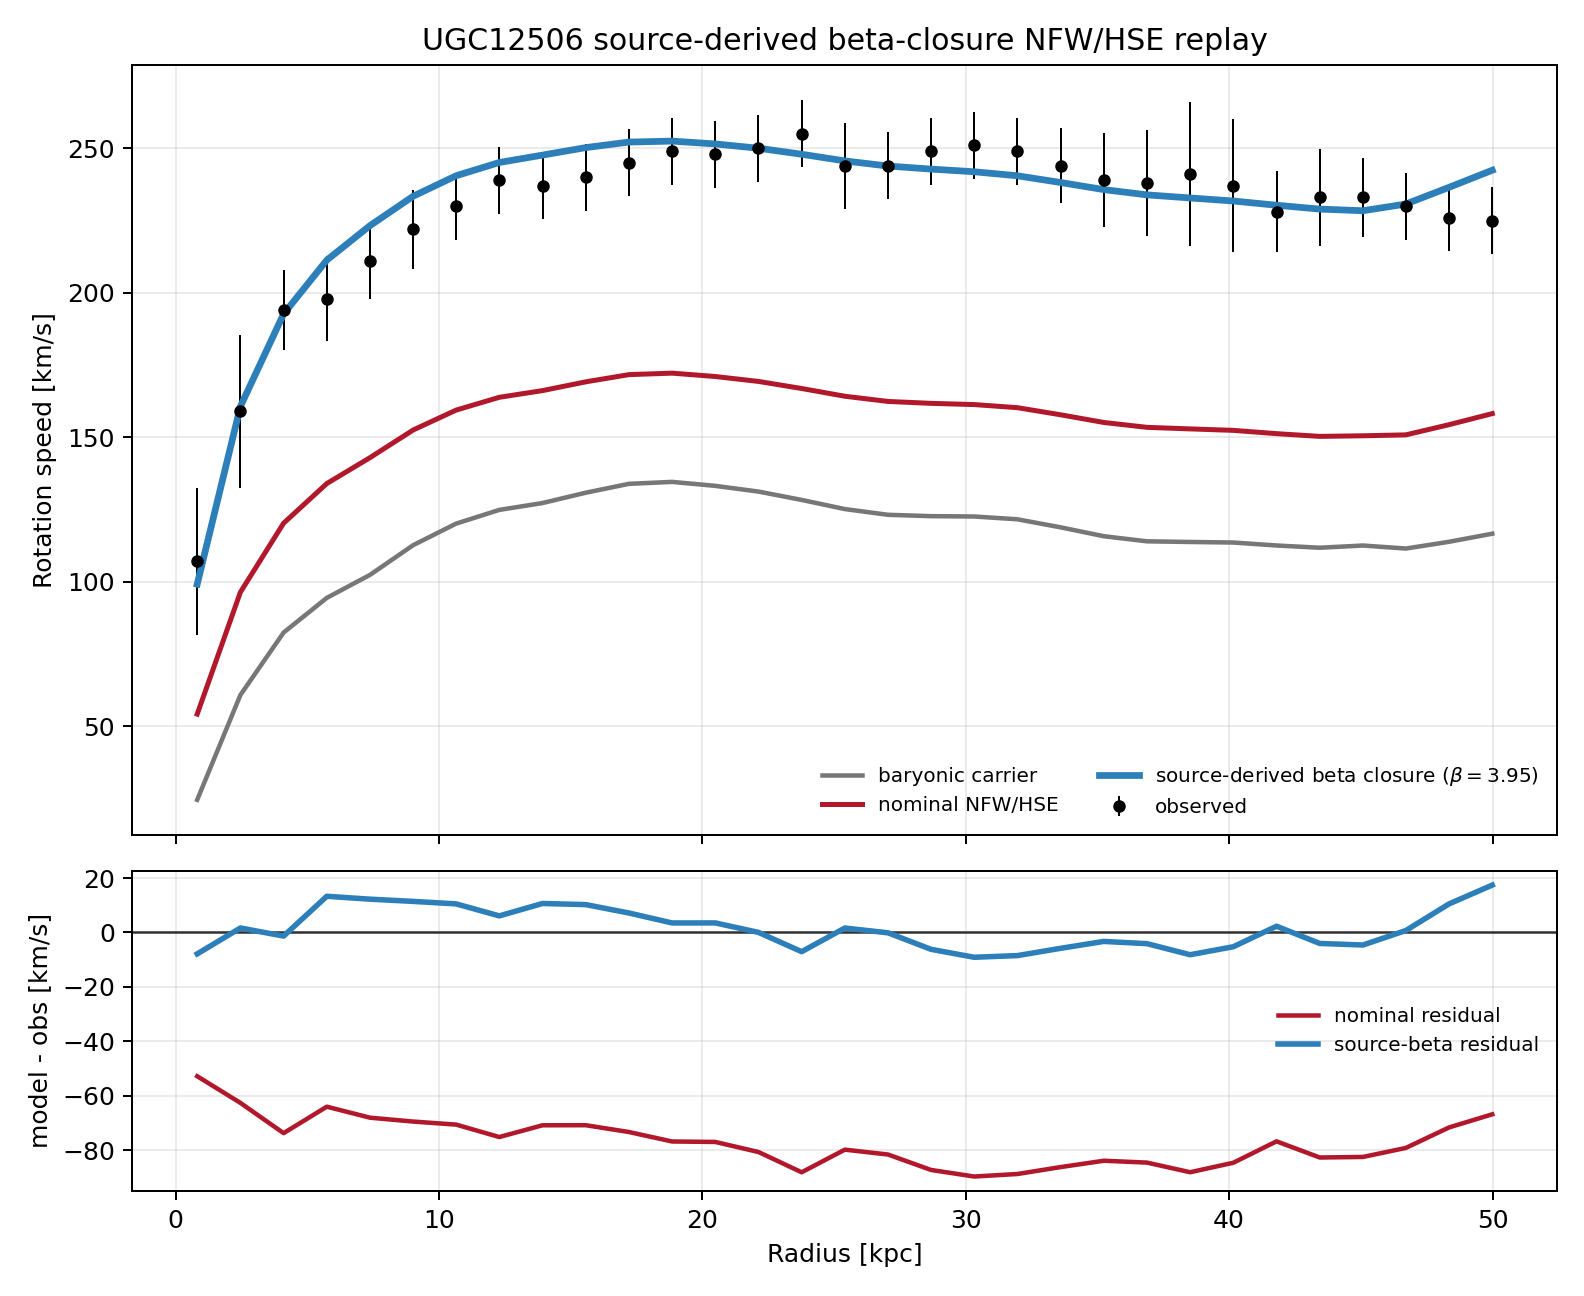
\includegraphics[width=\linewidth]{figures/fig30_ugc12506_source_derived_beta_closure_replay.png}
\caption{UGC12506 source-derived \(\beta_{\rm cl}\) closure replay.  The blue
curve uses a source-only beta factor from spin, source-native NFW preference,
and edge-on projection load.  It nearly reproduces the residual-aware
normalization scale and follows the observed curve closely, but remains a
post-diagnostic candidate until transferred to independent source-frozen
cases.}
\label{fig:ugc12506-source-beta-closure}
\end{figure}

The UGC12506 sequence is therefore a second morphology-refinement example,
but with a stronger caveat than the NGC0891/NGC4217 edge-on vertical/halo
controls.  Here the first six rows are source-frozen or ledger-strict control
replays, while the final \(\beta_{\rm cl}\) closure row is a
post-diagnostic source candidate.  The scientific use of the sequence is not
to claim that UGC12506 has been solved.  It is to show what a source-side
refinement ladder looks like when increasingly specific Tau morphology-state
channels are activated: baryonic carrier, envelope support, source-native
mass/envelope closure, observer/projection history, morphology-state phase,
and finally a clock/readout cap.

\begin{table}[H]
\centering
\small
\begin{tabularx}{\linewidth}{@{}r l r X@{}}
\toprule
Step & Readout curve & RMSE & Status \\
\midrule
1 & baryonic carrier & 116.02 & baseline/control carrier \\
2 & source envelope support & 102.48 & source-frozen envelope branch \\
3 & source-native NFW/HSE & 77.54 & source-native mass/envelope closure control \\
4 & projection/history increment & 69.18 & observer/projection-history control \\
5 & \(\Theta_{\rm morph}\) & 64.12 & Tau morphology-state phase diagnostic \\
6 & \(\Theta_{\rm morph}+\Xi_t\) cap & 60.31 & ledger-strict combined control \\
\midrule
7 & source \(\beta_{\rm cl}\) closure & 7.67 & post-diagnostic source candidate; not endpoint validation \\
\bottomrule
\end{tabularx}
\caption{UGC12506 morphology-refinement ladder.  Values are RMSE in
km\,s\(^{-1}\).  The ordered improvement is informative because each
pre-\(\beta_{\rm cl}\) step corresponds to an explicitly recorded source-side
channel or control artifact.  The final source \(\beta_{\rm cl}\) row is shown
to indicate the remaining amplitude/closure route, but it is not promoted to
endpoint evidence in this manuscript.}
\label{tab:ugc12506-morphology-refinement-ladder}
\end{table}

\begin{figure}[H]
\centering
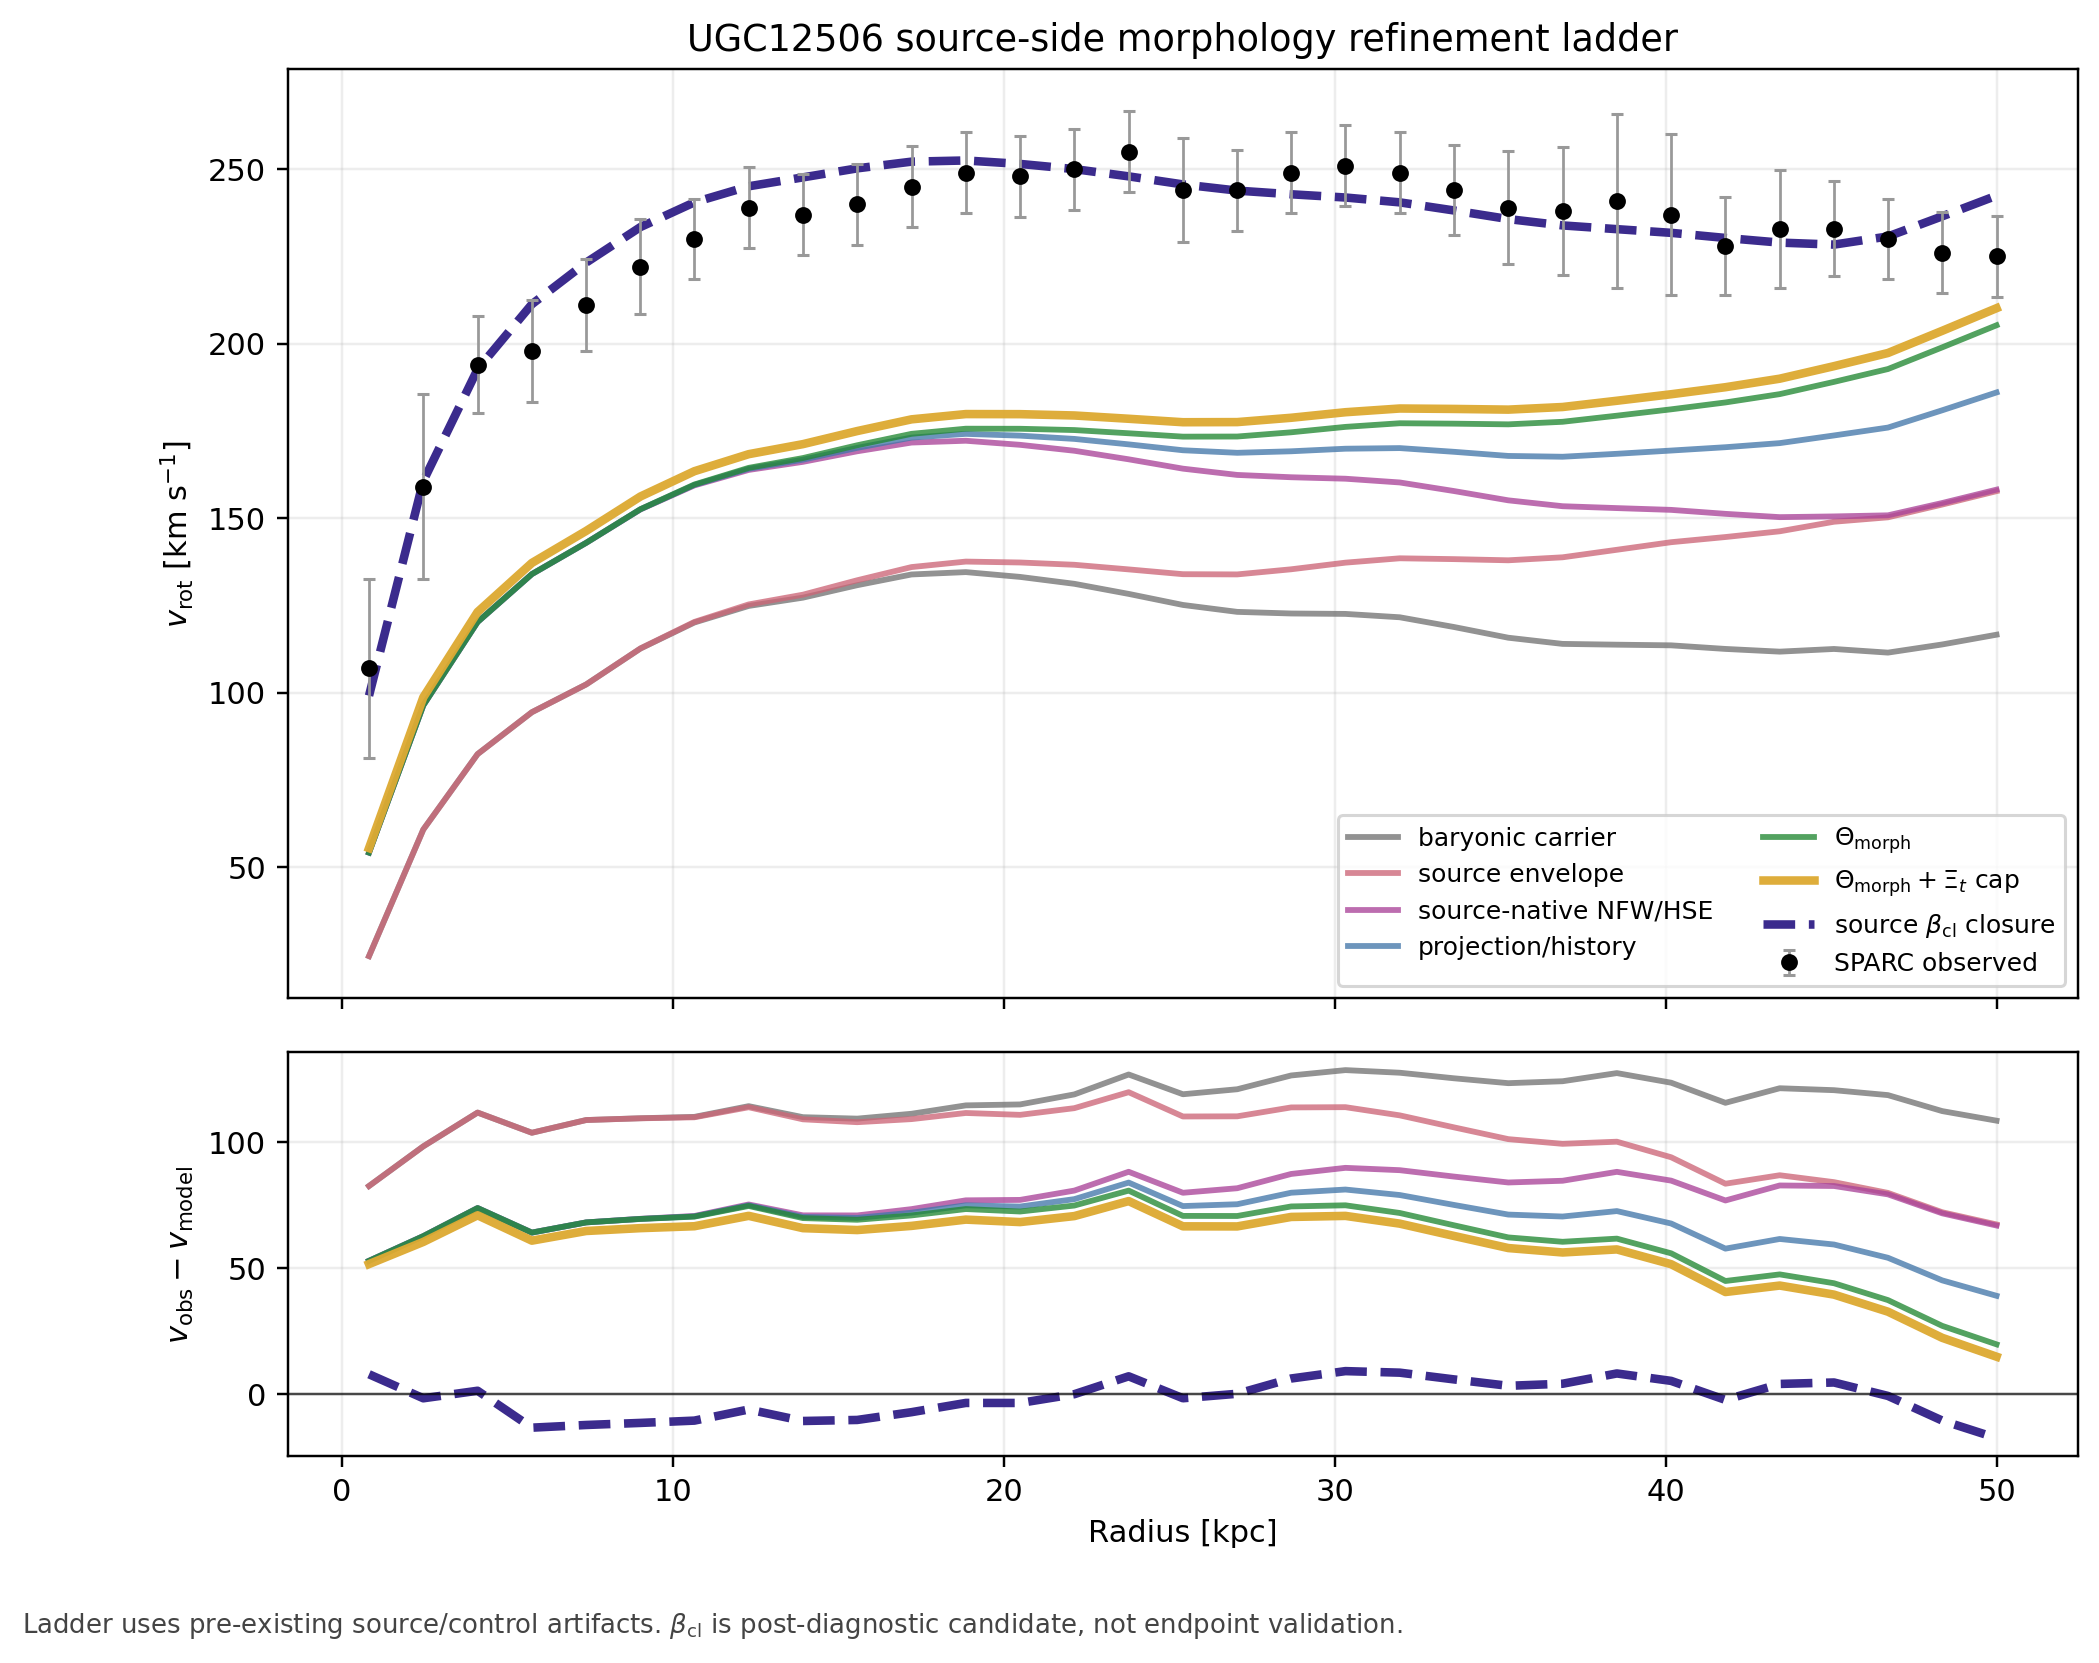
\includegraphics[width=\linewidth]{figures/fig31_ugc12506_morphology_refinement_ladder.png}
\caption{UGC12506 source-side morphology refinement ladder.  The curves move
progressively toward the observed rotation data as more specific source-side
readout channels are activated.  This is not curve fitting: the steps are
assembled from pre-existing source/control artifacts and the residuals are
used only for replay scoring.  The dashed \(\beta_{\rm cl}\) curve is the
post-diagnostic source-candidate closure route and is not counted as endpoint
validation.}
\label{fig:ugc12506-morphology-refinement-ladder}
\end{figure}

To prevent this encouraging result from becoming a same-galaxy rescue, we also
freeze an independent transfer predeclaration.  Using only SPARC source proxies
for inclination, \(R_{\rm HI}/R_d\), H~I mass, \(V_{\rm flat}\), and quality
flag, the transfer gate finds 11 non-UGC12506 candidates and authorizes no
replay score yet.  The top source-acquisition targets are UGC11455,
ESO563-G021, IC4202, NGC0891, NGC4013, NGC2841, NGC4157, and NGC4217.  Each
candidate must obtain source-native \(\lambda_{\rm spin}\), \(\chi^2_{\rm NFW}\),
\(\chi^2_{\rm ISO}\), halo-fit provenance, and PV/envelope notes before the
\(\beta_{\rm cl}\) rule can be replayed as an independent transfer test.
As a first blocker-reduction step, the Li et al. SPARC halo-fit catalogue
\cite{Li2020SPARCHaloCatalog} was used through VizieR to fill the pISO and NFW
reduced-\(\chi^2\) fields for all 11 predeclared candidates.  This does not
unlock replay, because \(\lambda_{\rm spin}\) and PV/envelope evidence remain
unfrozen, but it changes the practical transfer queue: the highest
edge-on/massive-H~I proxies are not necessarily UGC12506-like NFW-preference
objects.  In the current catalogue readout, positive NFW-preference load appears
most clearly for NGC0891, NGC7331, NGC2841, NGC0801, and weakly NGC4013.
The resulting priority gate therefore keeps NGC0891 and NGC7331 as the first
source-review targets for this specific \(\beta_{\rm cl}\) transfer route,
retains NGC2841, NGC0801, and NGC4013 as weak/secondary targets, and preserves
the pISO-preferred systems as controls or alternative-branch candidates rather
than forcing the UGC12506 normalization rule onto them.
The first source-freeze preflight for these two primary targets accepts
PV/envelope context for both objects, but freezes no direct
\(\lambda_{\rm spin}\) value.  Thus no \(\beta_{\rm cl}\) replay is authorized:
the next admissible step is either a direct source-native spin acquisition or a
predeclared source-only spin-proxy rule before any transfer residual is
inspected.
A direct-source search only partially reduces this blocker.  NGC7331 has a
published disc-spin-like value, \(\lambda=0.423\), in the lognormal
self-gravitating disc analysis of Marr \cite{Marr2015LognormalDiscAngularMomentum},
but that quantity is not the same as the halo/envelope \(\lambda_{\rm spin}\) slot used in the
\(\beta_{\rm cl}\) rule.  NGC0891 has no accepted direct source-native
\(\lambda_{\rm spin}\) value in the current cache; the available
NGC891-like spin context is model-analogue material only.  Therefore no direct
lambda source currently authorizes replay.
A follow-up NGC0891 source hunt strengthens the physical transfer motivation
but not the missing normalization slot.  Deep H~I and extraplanar-gas studies
show a massive lagging halo, low-angular-momentum accretion context, vertical
rotation gradients, and projection-sensitive halo modelling
\cite{Oosterloo2007ColdGaseousHaloNGC891,FraternaliBinney2006ExtraplanarGas,Fraternali2004ExtraPlanarNGC891,Ciotti2010StationaryExtraplanarGas}.
These are exactly the kind of source-side facts that make NGC0891 a relevant
halo/envelope transfer target, but none of them supplies the dimensionless
halo/envelope \(\lambda_{\rm spin}\) required by the \(\beta_{\rm cl}\) slot.
Thus the source hunt changes the interpretation from ``weak target'' to
``well-motivated but still normalization-blocked target'', not to a replay.
The explicit definition-conversion gate preserves this as a negative control:
the Marr value is accepted as source-side angular-momentum context, but direct
substitution is rejected.  If one inserted \(\lambda=0.423\) into the
\(\beta_{\rm cl}\) slot without conversion, the NGC7331 beta factor would be
\(1.73\), compared with \(1.23\) for the declared source-proxy candidate.  The
larger number is not a problem by itself; the problem is that no residual-blind
disc-to-halo/envelope conversion functional has been accepted.
As a conservative control, we also compute a Bullock-like disk-inferred spin
conversion proxy rather than relying only on the source-declared exposure
proxy.  Following the standard disk/halo angular-momentum normalization
logic \cite{MoMaoWhite1998DiscFormation,Bullock2001UniversalAngularMomentum},
we form
\[
  j_{\rm disk}=2R_dV_{\rm flat},\qquad
  R_{200}={V_{200}\over 10H_0},\qquad
  \lambda'_{\rm disk}
  =
  {j_{\rm disk}\over \sqrt{2}R_{200}V_{200}},
\]
using only source-side SPARC disk quantities and the Li et al. NFW-flat
\(V_{200}\) field.  This gate is dimensionless and residual-blind, but it is
not accepted as the Tau-side \(\beta_{\rm cl}\) halo/envelope spin slot.  It
gives \(\lambda'_{\rm disk}=0.035\) for NGC0891 and \(0.033\) for NGC7331,
substantially below the corresponding source-declared exposure-proxy values
\(0.149\) and \(0.136\).  The disagreement is scientifically useful: it means
the replay cannot be reopened by a hidden amplitude choice.  An independent
review must choose direct spin acquisition, the exposure proxy, the
Bullock-like conversion proxy, or rejection of the transfer route before any
\(\beta_{\rm cl}\) replay.
We implement the second option only as a blocker-reduction gate.  The declared
proxy uses bounded source loads from \(R_{\rm HI}/R_d\), \(V_{\rm flat}\), H~I
mass, and inclination,
\[
  \lambda_{\rm spin,proxy}
  =
  0.10\left[
    1 + 0.35 L_{\rm extent}
      + 0.25 L_V
      + 0.25 L_{\rm gas}
      + 0.15 L_{\rm edge}
  \right],
\]
and combines it with the already frozen NFW-preference load only to prioritize
independent source review.  This gate selects NGC0891 as the only primary
proxy-transfer review target and keeps NGC7331, NGC2841, NGC0801, and NGC4013
as secondary targets.  It is not accepted as a direct
\(\lambda_{\rm spin}\) measurement and still authorizes no replay or endpoint
score.
For reproducibility and leakage prevention, this proxy route is packaged as an
independent review bundle rather than silently promoted.  The bundle contains
the declared proxy fields, transfer queue, direct-source audit,
definition-conversion rejection, the Bullock-like conversion-control files,
forbidden inputs, review obligations, and a blank response form.  Its current
status is
\texttt{READY\_RESPONSE\_PENDING}: the reviewer may accept the source fields,
choose the exposure proxy, choose the Bullock-like disk-conversion proxy,
require direct source-native spin, require a new residual-blind rule, keep the
Marr NGC7331 value as context only or supply a genuine conversion rule, and
restrict the transfer target set.  The
bundle itself still sets \(\texttt{beta\_cl\_replay\_allowed=false}\) and
\(\texttt{endpoint\_scores\_allowed=false}\).  Thus the proxy is reviewable
without residual leakage, but not yet an accepted Tau-side amplitude law.
A companion response-intake validator is also present.  With no completed
external response currently supplied, it records
\(\texttt{RESPONSE\_PENDING\_ENDPOINT\_BLOCKED}\), with
\(\texttt{selected\_spin\_normalization\_route}\) still pending.  Until such a
route is independently accepted, proxy promotion, \(\beta_{\rm cl}\) replay
preflight, and endpoint scoring all remain disabled.
The downstream spin-route prefreeze gate is already implemented and currently
records
\(\texttt{SPIN\_ROUTE\_PREFREEZE\_BLOCKED\_REVIEW\_ROUTE\_PENDING}\), emitting
no transfer values.  Thus the paper has a concrete replay lock rather than an
informal caveat.
We also expose this lock as a four-row route-decision matrix.  The available
decisions are the source-declared exposure proxy, the Bullock-like disk
conversion proxy, a future direct source-native spin measurement, or rejection
of the route.  The first two are computable but reviewable-not-accepted; the
third is scientifically preferred but currently missing; the fourth is a valid
route-level negative outcome.  None of the four rows authorizes endpoint
scoring.
Finally, the beta-closure scoring launch gate is already present.  It finds
that all nine required launch inputs exist, but the review-route acceptance,
prefreeze-value, and carrier-freeze gates are still blocked.  The protocol
skeleton therefore identifies the future scoring script as the only step
allowed to read \(v_{\rm obs}\), and keeps that step inactive until a
source-frozen formula manifest exists.
The additional carrier-freeze gate is needed because \(\beta_{\rm cl}\) is an
amplitude/closure factor, not a complete rotation-curve formula by itself.  It
records three possible carrier routes: a reviewable but not yet accepted
baryonic-fast-packet stress carrier, a Li et al. NFW-fit diagnostic/control
carrier, and the preferred but currently missing source-native NFW/HSE transfer
carrier.  The Li et al. route is useful for context and controls, but it is not
endpoint-safe by default because its halo parameters are published
rotation-curve fit products.
This blocker is now converted into an explicit review packet rather than left
as an informal caveat.  The carrier review bundle contains the route decision
matrix, source artifacts, forbidden-input ledger, and a blank response form.
The response intake currently records
\(\texttt{CARRIER\_REVIEW\_RESPONSE\_PENDING\_ENDPOINT\_BLOCKED}\).  A future
independent response may accept the minimal baryonic stress carrier, require a
source-native transfer carrier, or reject the route, but it may not use
endpoint residuals or baseline ranks to choose the carrier.
We now also instantiate that intermediate formula-freeze gate explicitly.  The
gate writes the transfer formula manifest path with headers and zero rows,
passes the halo-fit and priority-field checks, but blocks on independent
route-review acceptance, source-frozen spin-route values, and an accepted
carrier.  Its status is
\(\texttt{TRANSFER\_FORMULA\_FREEZE\_BLOCKED\_PREFREEZE\_PENDING}\).  In other
words, the formula shell
\[
  \beta_{\rm cl}
  =
  1+
  {\lambda_{\rm spin}\over 0.10}L_{\rm NFW}
  +L_{\rm edge}
\]
is present as a declared transfer form, but no galaxy row is frozen into the
manifest until the spin-normalization route is independently accepted.  This
gate reads no observed rotation curve and produces no score.
The separate transfer scoring runner has also been added; in the current state
it exits with
\(\texttt{TRANSFER\_SCORING\_BLOCKED\_LAUNCH\_GATE}\), writes an empty score
table, sees the existing but empty formula manifest, and reads no observed
rotation curve.  The dormant control-scoring branch is implemented for a future
accepted \(\texttt{BARYONIC\_050\_FAST\_PACKET}\) carrier: after the launch and
formula-freeze gates pass, it computes
\[
v_{\rm readout}(R)=\sqrt{\beta_{\rm cl}\,v_{\rm baryon,0.5}^{2}(R)}
\]
and writes both score-level and point-level artifacts.  This keeps the
score-producing stage technically present but leakage-locked.
Finally, a no-\(v_{\rm obs}\) scoring-contract dry run is now generated.  It
does not accept either review route and does not score.  Instead, it asks
whether the already implemented spin routes and the reviewable baryonic stress
carrier would have enough non-observed inputs to execute if later accepted by
independent review.  The current dry run reports two contract-ready scenarios:
\(\texttt{EXPOSURE\_PROXY}\) and
\(\texttt{BULLOCK\_DISK\_CONVERSION}\), both paired with
\(\texttt{BARYONIC\_050\_FAST\_PACKET}\).  It writes 22 dry-run manifest rows
and 656 prediction rows without reading observed velocities or residuals.
Thus the remaining blocker is review/freeze authorization, not missing scoring
infrastructure.
The final pre-scoring handoff is an unlock packet with exact active-response
requirements for the spin-route and carrier reviews.  It includes example-only
CSV rows for the two spin-route choices and the baryonic stress carrier, but it
does not create active response files.  Scoring remains blocked until an
independent reviewer supplies those active files and the standard intake,
prefreeze, formula-freeze, and launch gates pass.
A post-review scoring launcher now runs that entire chain as one command.  In
the present package all chain scripts return successfully, but the launcher
keeps the scoring runner blocked because zero active reviewer response files
are present.  Thus the scoring path is mechanically ready, while the scientific
authorization remains external-review gated.
To avoid accidental promotion of example rows, active reviewer responses are
installed only through a validator that checks the incoming CSV schemas,
rejects \(\texttt{EXAMPLE\_ONLY}\) or pending rows, rejects endpoint/residual
flags, and copies the files into the active paths only if both responses pass.
In the present package the installer reports zero incoming active responses and
therefore installs nothing.
The current release also writes a scoring-readiness dashboard that condenses
the dry-run contract, unlock packet, active-response installer, launcher,
launch gate, formula-freeze gate, and dormant scoring runner into a single
ledger.  That ledger reports the present status as
\(\texttt{SCORING\_READINESS\_BLOCKED\_ACTIVE\_RESPONSES\_PENDING}\):
the no-\(v_{\rm obs}\) contract and unlock packet are ready, but no score is
authorized and no observed rotation curve is read until the two active review
responses are supplied and validated.
Thus the present result is a strong post-diagnostic derivation candidate, while
the validation path is explicitly shifted to independent source acquisition.

\section{Source-blind morphology refinement controls}
\label{sec:transfer-refinement}

\subsection{Beta-transfer lock-type review and refinement ladder}
\label{subsec:morphology-refinement-ladder}

The beta-transfer work also gives a useful example of how morphology
refinement should be carried out without becoming curve fitting.  The
refinement is not allowed to choose a curve because the curve looks better.
Instead, the only admissible sequence is:
\[
  \hbox{source morphology review}
  \;\rightarrow\;
  \hbox{frozen readout family}
  \;\rightarrow\;
  \hbox{control replay}
  \;\rightarrow\;
  \hbox{score}.
\]
The replay score may trigger a review, but it may not decide which
morphology-family replacement is used.  The source-side replacement must be
justified from independent observations such as inclination, dust lanes,
extra-planar gas, radio/halo emission, H~I support, or published
projection/vertical-structure studies.
This section is not evidence for beta closure.  It is a methodological control
showing how failed transfer branches are handled without residual-driven
refitting: the failed pure branch is preserved, and a replacement branch is
allowed only after source-side morphology review.

The current beta-transfer control illustrates the full ladder.  The global
closure-transfer branch
\[
  v_{\beta}^{2}(R)=\beta_{\rm cl}\,v_{\rm carrier}^{2}(R)
\]
is a deliberately blunt control: it asks whether the UGC12506-inspired
closure normalization can be transported as a whole.  For NGC0891 and
NGC4217 this pure branch fails by overshooting.  That failure is preserved as
a negative branch-level control, not hidden.  The residual-blind source review
then asks a different question: are these galaxies actually pure
beta/compact-transfer cases, or are they edge-on vertical/halo systems whose
readout should be spatially gated?  The source ledger rejects the pure
beta/compact primary lock for both rows and supports an edge-on
vertical/dust/H~I/radio-halo mixed interpretation, using independent
edge-on dust, H~I halo, extra-planar gas, and radio/halo evidence
\cite{NASA2024NGC891EdgeOnBeauty,HowkSavage1997NGC891Dust,
Oosterloo2007ColdGaseousHaloNGC891,ESA2015NGC4217Hubble,
Heesen2024NGC4217Changers}.  The exact review artifacts are
\texttt{data/derived/beta\_transfer\_source\_side\_morphology\_review\_gate.csv}
and
\texttt{data/derived/beta\_transfer\_lock\_type\_source\_review.csv}.

The first source-locked refinement is therefore not a new amplitude fit but an
edge-on vertical/halo gate:
\[
  v_{\rm EVH}^{2}(R)
  =
  v_{\rm carrier}^{2}(R)
  \left[1+(\beta_{\rm cl}-1)K_{\rm EVH}(R)\right],
\]
where
\[
  K_{\rm EVH}(R)
  =
  {\rm smoothstep}\!\left(
    {R-R_{\rm on}\over R_{\rm full}-R_{\rm on}}
  \right),
  \qquad
  R_{\rm on}=2R_s,\quad
  R_{\rm full}=\min(3R_s,R_{\max}).
\]
This version says that the transferred closure load should become active only
where the source-side edge-on vertical/halo component is expected to project
strongly into the rotation readout.  It improves both galaxies relative to the
carrier and avoids the pure global-beta overshoot.

The second refinement follows a further source-side observation: the vertical
dust/halo and extra-planar gas evidence for these edge-on systems is not only
an extreme outer-tail feature.  It is distributed over the disk/halo interface.
That motivates a distributed vertical/halo gate,
\[
  v_{\rm DVH}^{2}(R)
  =
  v_{\rm carrier}^{2}(R)
  \left[1+(\beta_{\rm cl}-1)K_{\rm DVH}(R)\right],
\]
with
\[
  K_{\rm DVH}(R)
  =
  {\rm smoothstep}\!\left({R-R_s\over 2R_s-R_s}\right).
\]
Again, the radial window is not chosen by minimizing the rotation-curve
residual.  It is the predeclared translation of the source claim that the
vertical/halo component is distributed through the disk-halo interface rather
than activated only at the far edge.

\begin{table}[H]
\centering
\small
\begin{tabularx}{\linewidth}{@{}lrrrrX@{}}
\toprule
Galaxy & Carrier & Pure \(\beta\) & EVH & DVH & Source-side interpretation \\
\midrule
NGC0891 & 44.15 & 74.35 & 30.20 & 23.07 &
Pure global beta overshoots; edge-on dust/H~I halo and extra-planar gas
support vertical/halo gating, with distributed activation preferred by the
source morphology. \\
NGC4217 & 47.62 & 55.00 & 37.66 & 27.23 &
Pure global beta remains too blunt; edge-on vertical/radio-halo context
supports a mixed vertical/halo readout, with distributed activation improving
the replay. \\
\bottomrule
\end{tabularx}
\caption{Morphology-refinement ladder for the beta-transfer control rows.
Entries are RMSE values in km\,s\(^{-1}\).  The table is a control replay, not
population validation.  The important feature is the ordered improvement:
source review rejects the pure branch, freezes a more specific morphology
family, and only then scores the replay.}
\label{tab:beta-transfer-morphology-refinement-ladder}
\end{table}

\begin{figure}[H]
\centering
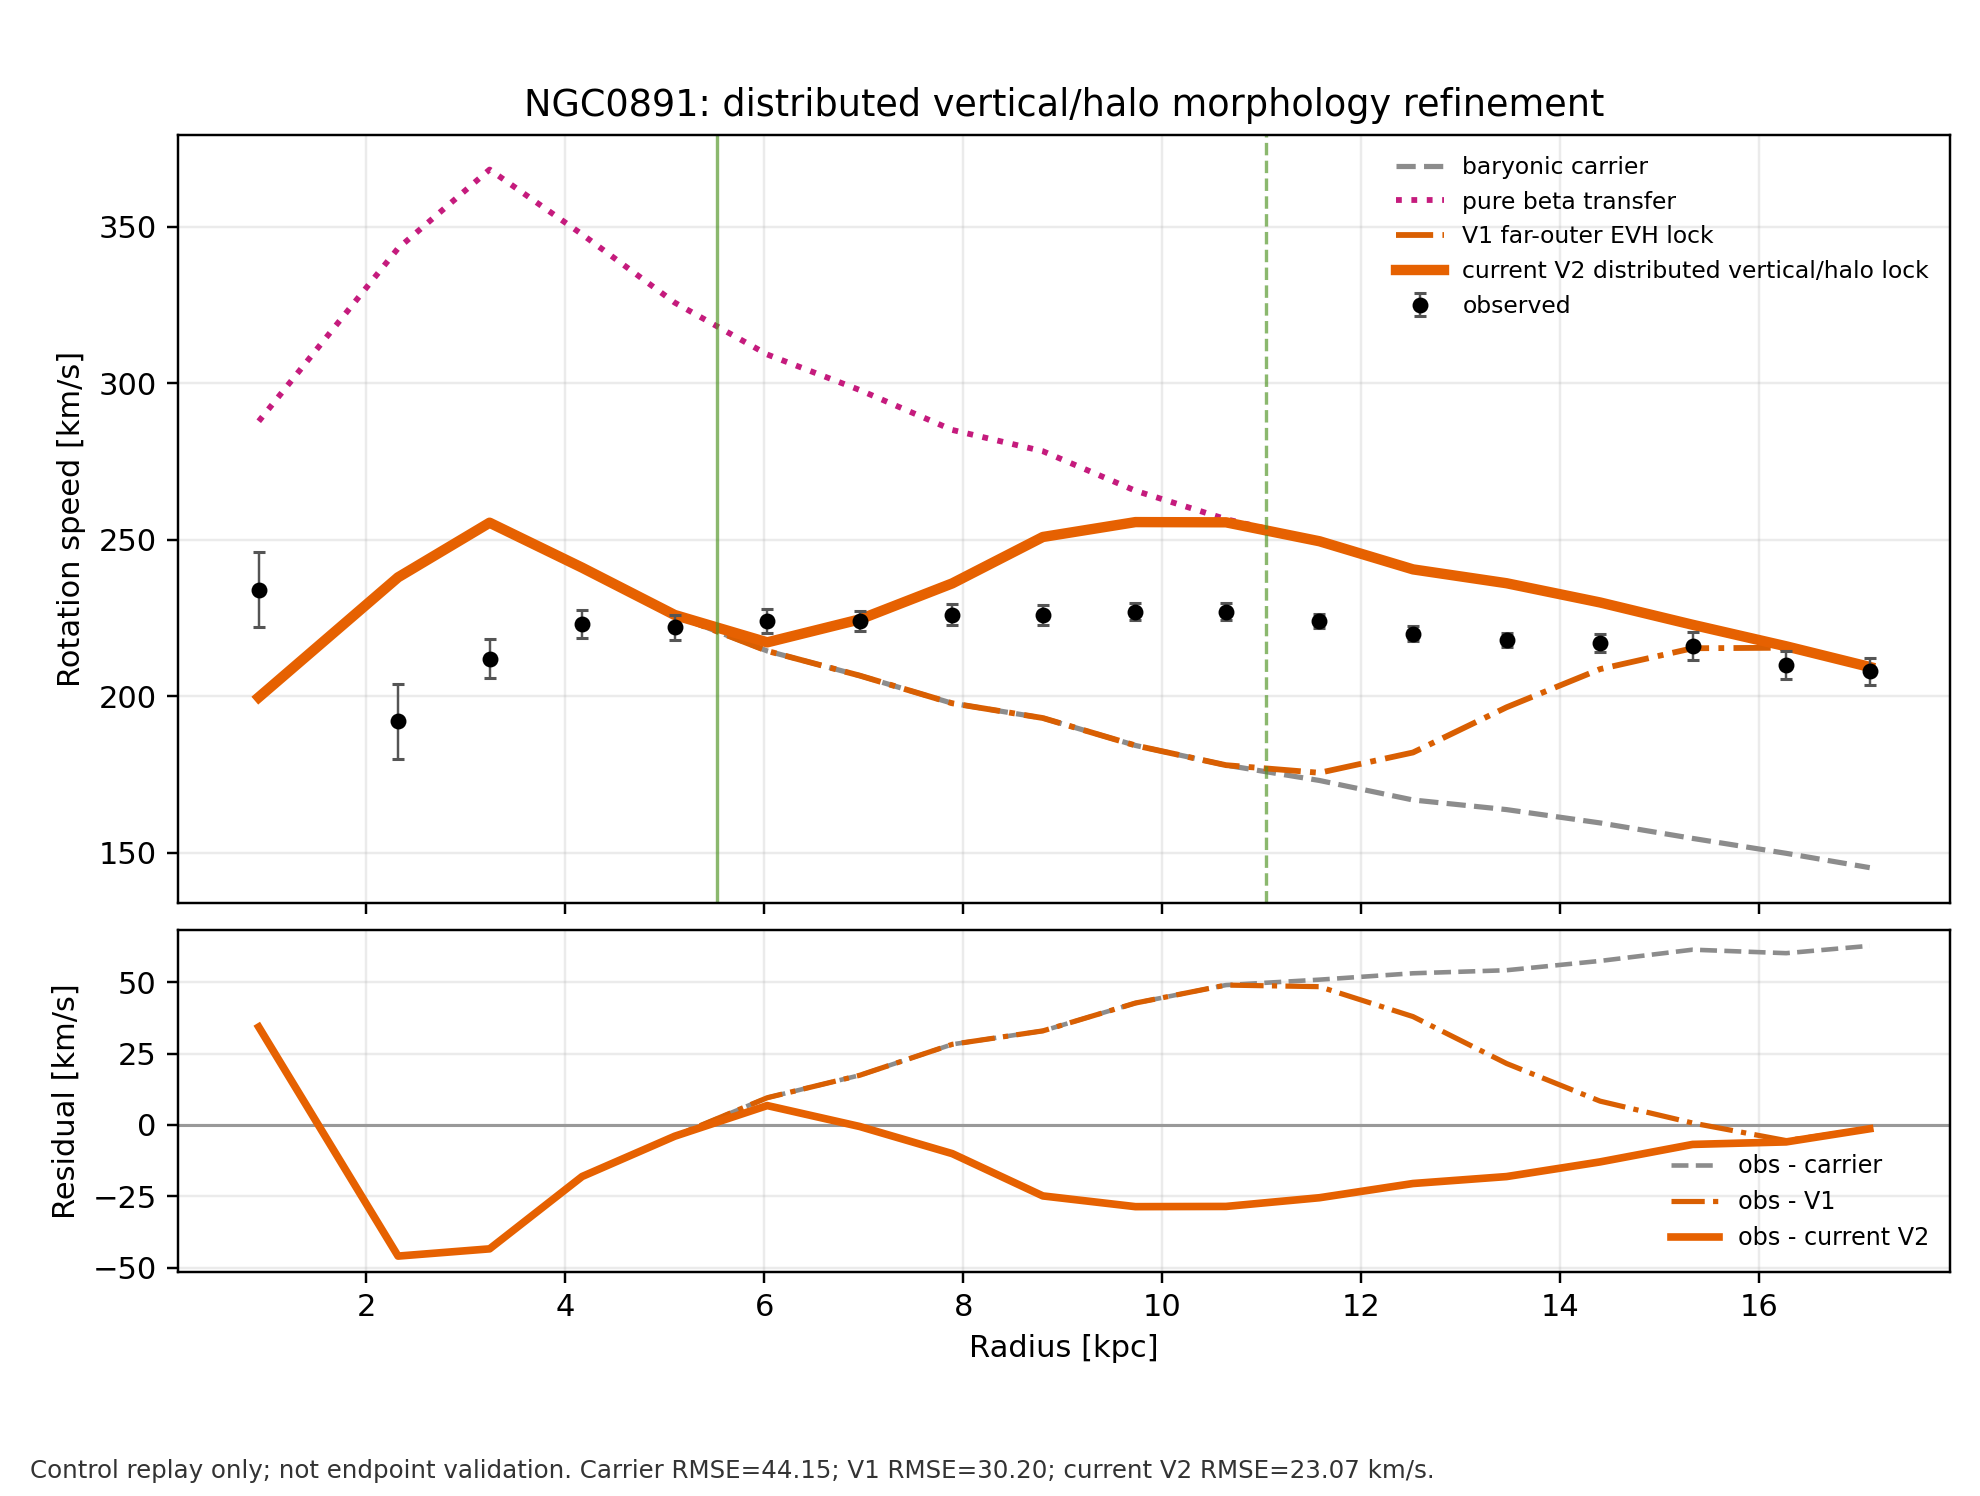
\includegraphics[width=\linewidth]{figures/fig_beta_transfer_distributed_vertical_halo_ngc0891.png}
\caption{NGC0891 morphology-refinement replay.  The pure beta-transfer branch
overshoots, while the source-frozen edge-on vertical/halo and distributed
vertical/halo kernels progressively move the predicted curve toward the
measured rotation data.  The refinement is source-side: the lock-type review
uses edge-on dust, extra-planar gas, and H~I halo evidence, not the residual
shape, to replace the pure branch.}
\label{fig:ngc0891-morphology-refinement}
\end{figure}

\begin{figure}[H]
\centering
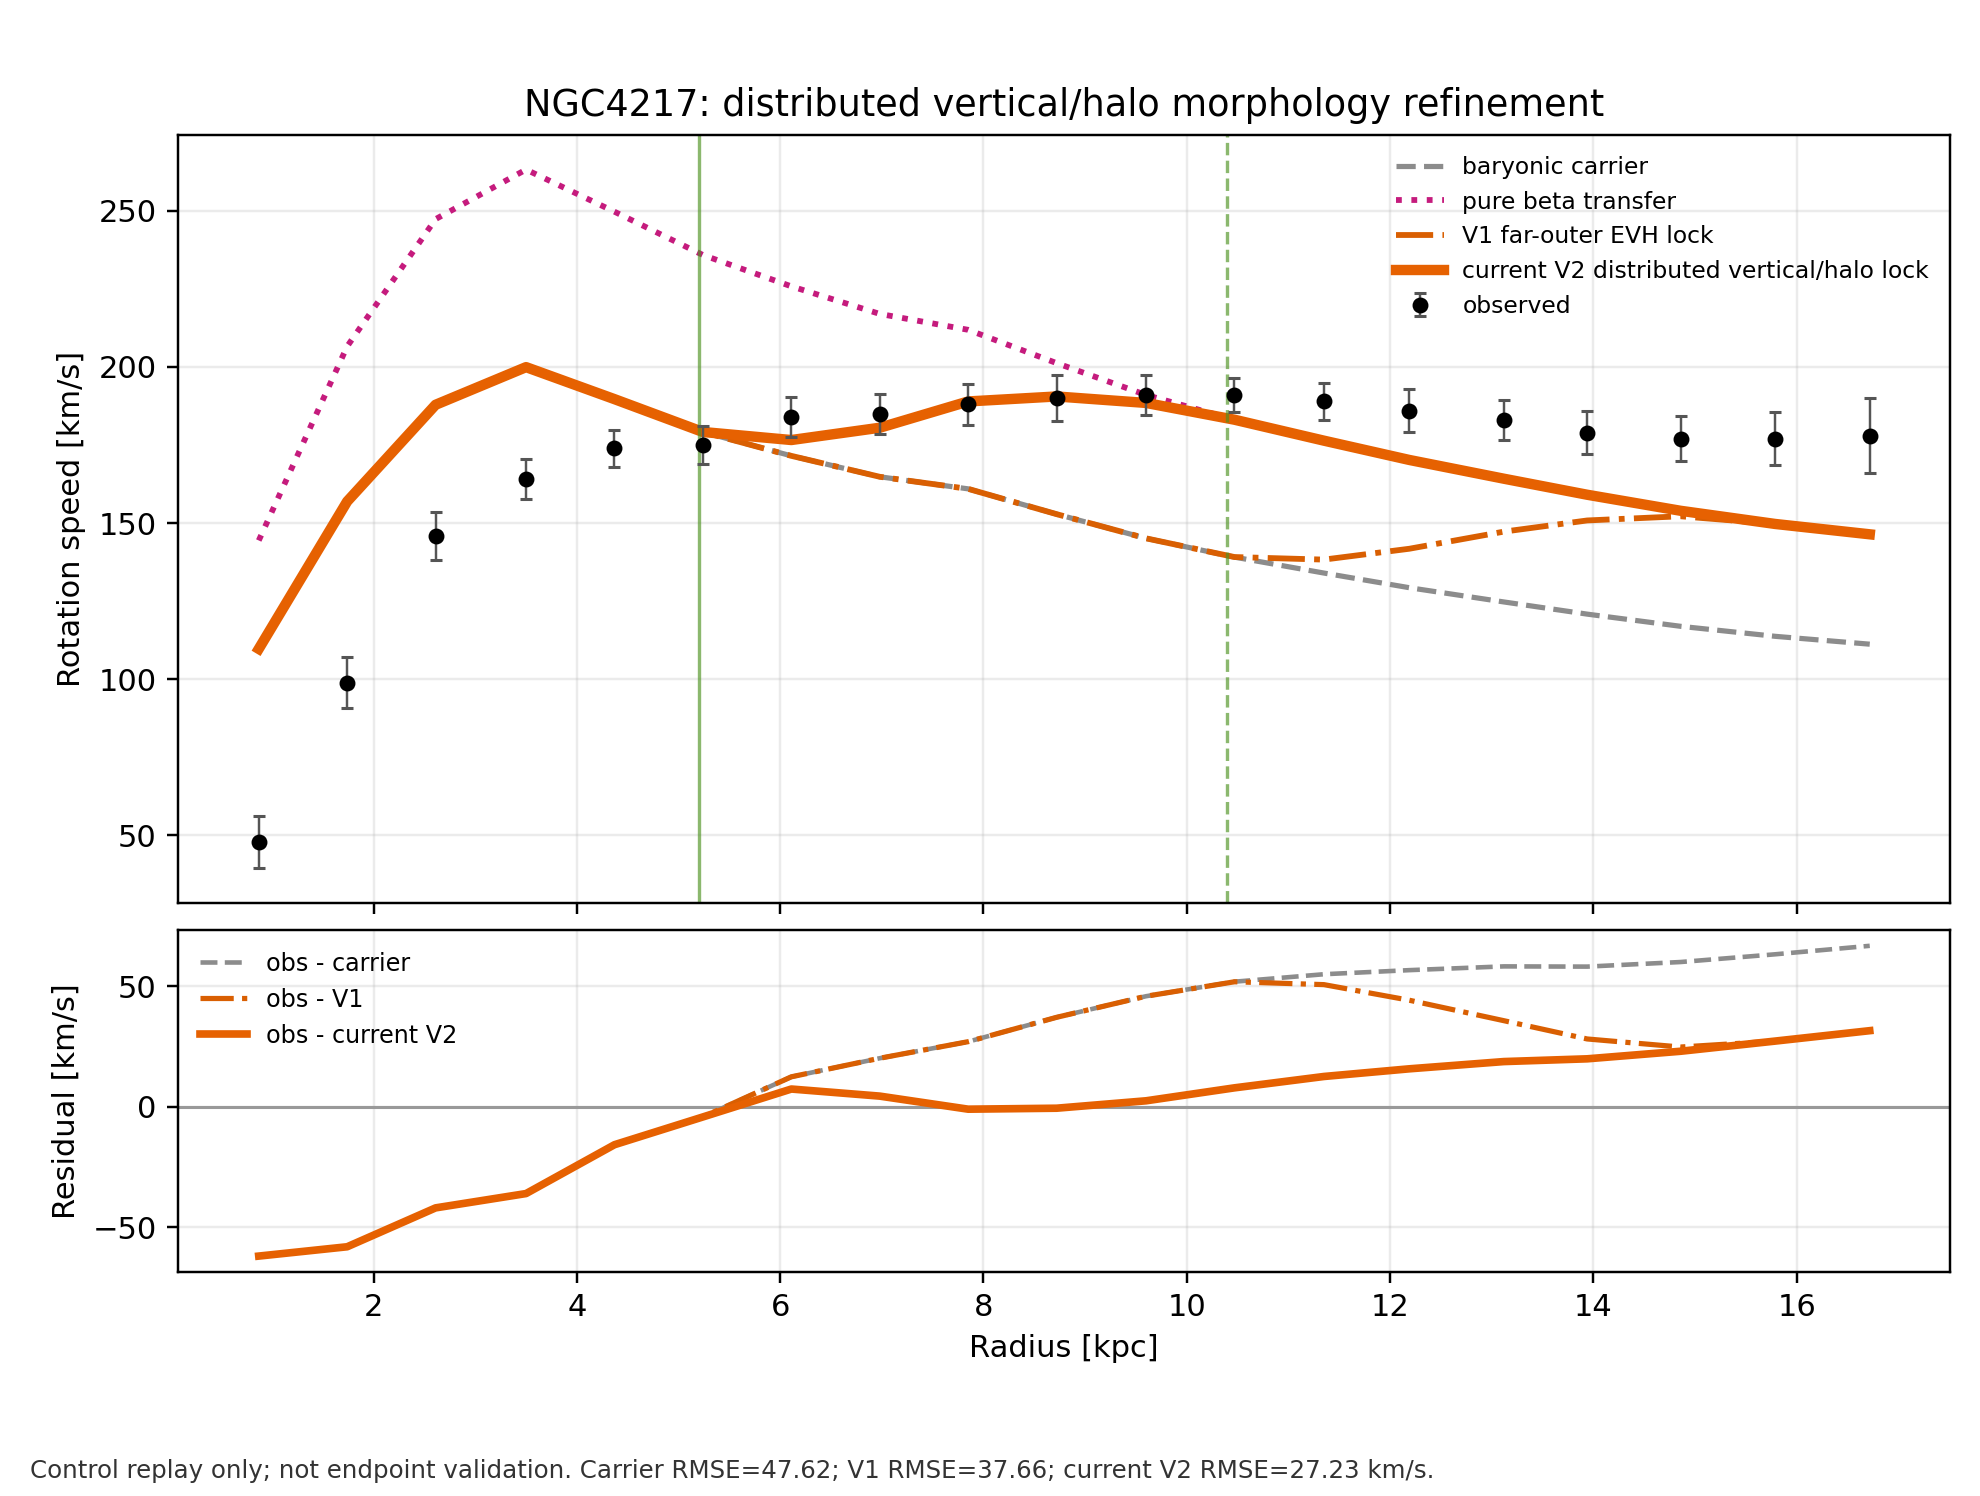
\includegraphics[width=\linewidth]{figures/fig_beta_transfer_distributed_vertical_halo_ngc4217.png}
\caption{NGC4217 morphology-refinement replay.  As in NGC0891, the curve
improves when the pure closure-transfer branch is replaced by a
source-supported edge-on vertical/halo readout, and improves further when the
vertical/halo contribution is treated as distributed through the disk-halo
interface.  This is a morphology-refinement control, not an endpoint claim.}
\label{fig:ngc4217-morphology-refinement}
\end{figure}

This ladder is important for the interpretation of failures.  A bad replay is
not automatically a Tau Core failure, and it is not automatically an invitation
to refit.  It is a source-review trigger.  If independent observations support
a more precise readout-relevant morphology, a replacement family may be
frozen and replayed.  If they do not, the failed branch remains a negative
control.  In this sense the paper tests a stronger operational claim than
``can a curve be made to fit'': it tests whether progressively more
source-complete, residual-blind morphology descriptions select kernels whose
rotation readouts follow the measured curves more closely.

\subsection{Additional refinement patterns: positive, guardrail, and caveated cases}
\label{subsec:additional-refinement-patterns}

The same source-blind refinement logic appears in three other inspected
systems, but with different scientific meanings.  NGC4088 is the clearest
positive projection/history case: adding the independently motivated
warp/history layer improves the replay, while the stronger additive-plus-clock
stress curve is kept as a control because its source channels overlap under
the source-token priority protocol of
Subsection~\ref{subsec:source-token-priority}.
NGC4013 is a guardrail case: moving from a simple compact proxy to a
warp/vertical-overlay family improves the readout, but adding an extra
\(\Xi_t\) overlay worsens the current proxy and therefore warns against
double-counting the same projected vertical/warp evidence; by the same
protocol, the vertical/warp source token is consumed by the mixed morphology
kernel unless an independent clock/readout separator is supplied.  NGC7331 is a
caveated source-sharpening case: a broad outer-warp window already improves
over the simple carrier, and a sharper source-window replay gives a small
additional gain, but the broad-window uncertainty remains part of the
accepted interpretation.

\begin{table}[H]
\centering
\small
\begin{tabularx}{\linewidth}{@{}llrX@{}}
\toprule
Galaxy & Source-frozen replay step & RMSE & Interpretation \\
\midrule
NGC4088 & Base projection & 11.62 &
Source-supported projection control. \\
NGC4088 & Additive warp/history & 9.39 &
Accepted projection/history refinement. \\
NGC4088 & Clock-only control & 10.50 &
Clock replay retained as a control, not an endpoint. \\
NGC4088 & Additive plus clock stress & 8.38 &
Lower RMSE, but source-channel overlap keeps it as a stress control. \\
\midrule
NGC4013 & Compact proxy & 16.99 &
Original simple morphology proxy. \\
NGC4013 & Warp/vertical overlay & 11.45 &
Source-supported mixed morphology refinement. \\
NGC4013 & Exponential-disk plus WVO protocol & 10.61 &
Prospective source-frozen protocol reference. \\
NGC4013 & \(\Xi_t\) overlay control & 12.04 &
Double-counting guardrail; worsens the current proxy. \\
\midrule
NGC7331 & Exponential-disk carrier & 23.47 &
Simple broad projected-disk carrier. \\
NGC7331 & V1 broad outer warp & 22.26 &
Accepted broad-window reference. \\
NGC7331 & V2 fractional onset & 22.73 &
Control replay; not the best source sharpening. \\
NGC7331 & V3 source-sharpened & 22.13 &
Small source-sharpened outer-warp gain. \\
NGC7331 & Wrong sharpened control & 22.91 &
Wrong-projection control, worse than the source-sharpened replay. \\
\bottomrule
\end{tabularx}
\caption{Additional morphology-refinement patterns.  Entries are RMSE values
in km\,s\(^{-1}\).  These rows are not an independent validation sample.
They show how a residual-blind source review can sharpen a readout family,
and also how the protocol blocks over-layering when a projection/time channel
would double-count the same source evidence.  The generating artifact is
\texttt{data/derived/additional\_morphology\_refinement\_ladders\_summary.csv}.}
\label{tab:additional-morphology-refinement-patterns}
\end{table}

\begin{figure}[H]
\centering
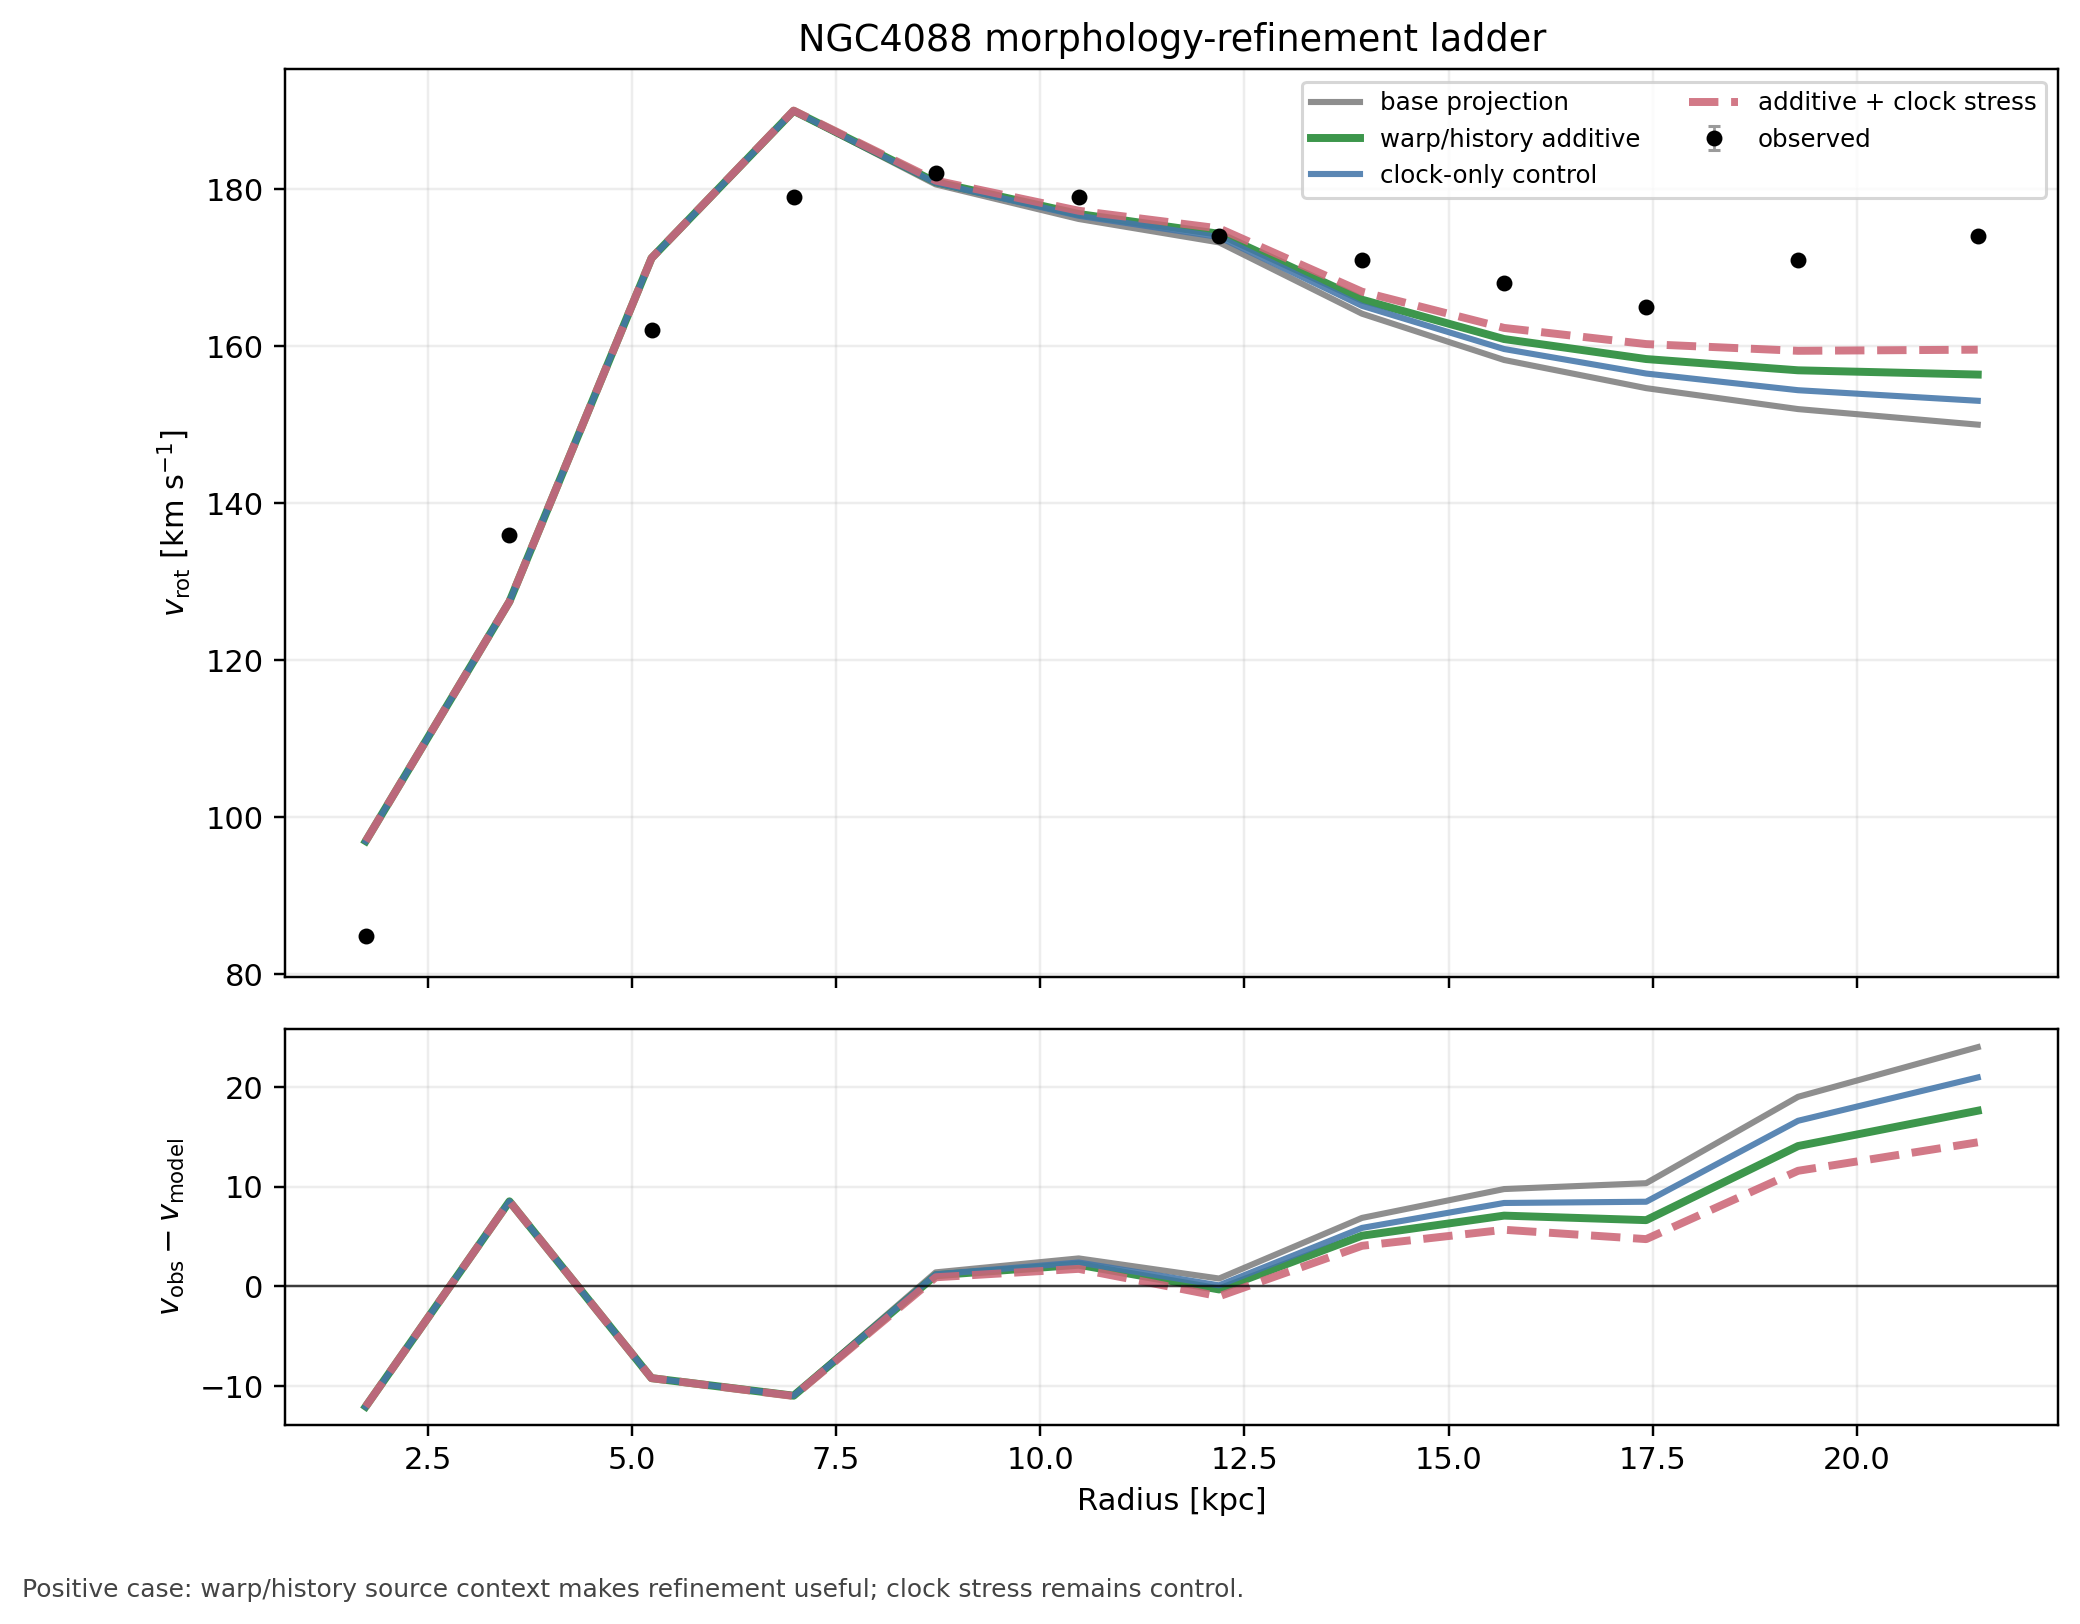
\includegraphics[width=\linewidth]{figures/fig_ngc4088_morphology_refinement_ladder.png}
\caption{NGC4088 projection/history refinement ladder.  The source-supported
warp/history layer moves the Tau Core replay closer to the measured rotation
curve.  The additive-plus-clock stress curve is shown because it lowers RMSE
further, but it is not promoted to endpoint validation: it overlaps source
channels and therefore remains a control.}
\label{fig:ngc4088-morphology-refinement-ladder}
\end{figure}

\begin{figure}[H]
\centering
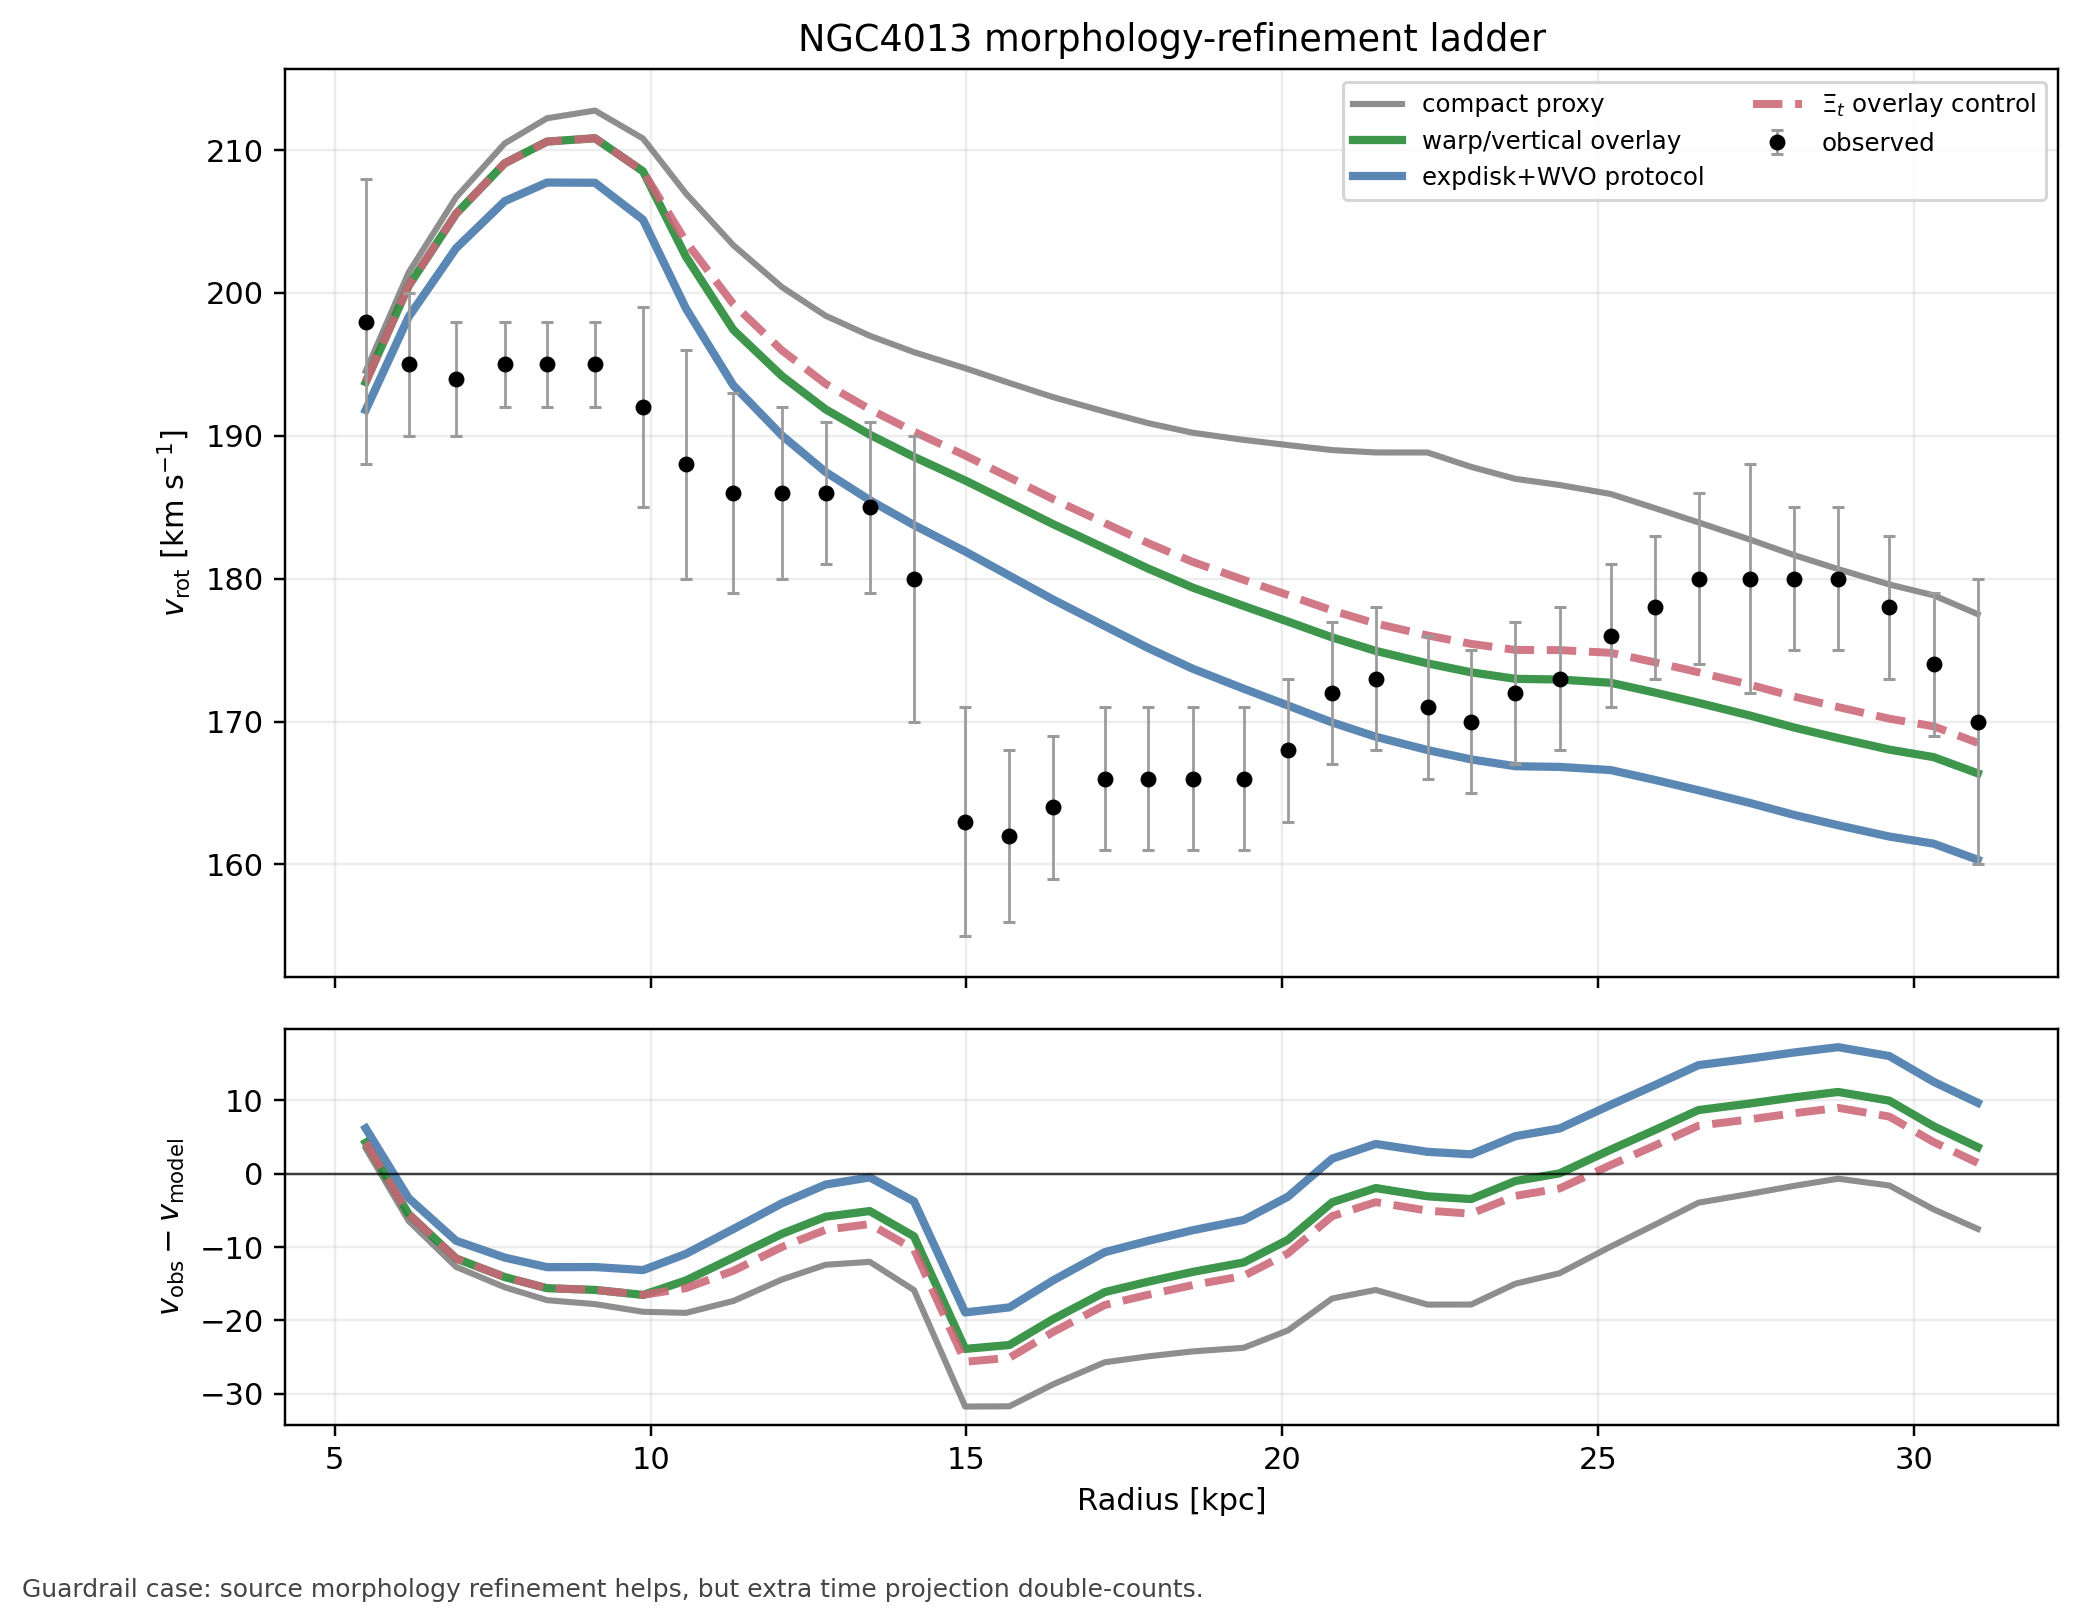
\includegraphics[width=\linewidth]{figures/fig_ngc4013_morphology_refinement_guardrail.png}
\caption{NGC4013 morphology-refinement guardrail.  The source-supported
warp/vertical-overlay route improves over the simple compact proxy, and the
prospective exponential-disk plus WVO protocol is closer still.  The
\(\Xi_t\) overlay control worsens the replay, illustrating that the
projection/time layer is not a universal improvement term and must not
double-count the same vertical/warp evidence.}
\label{fig:ngc4013-morphology-refinement-guardrail}
\end{figure}

\begin{figure}[H]
\centering
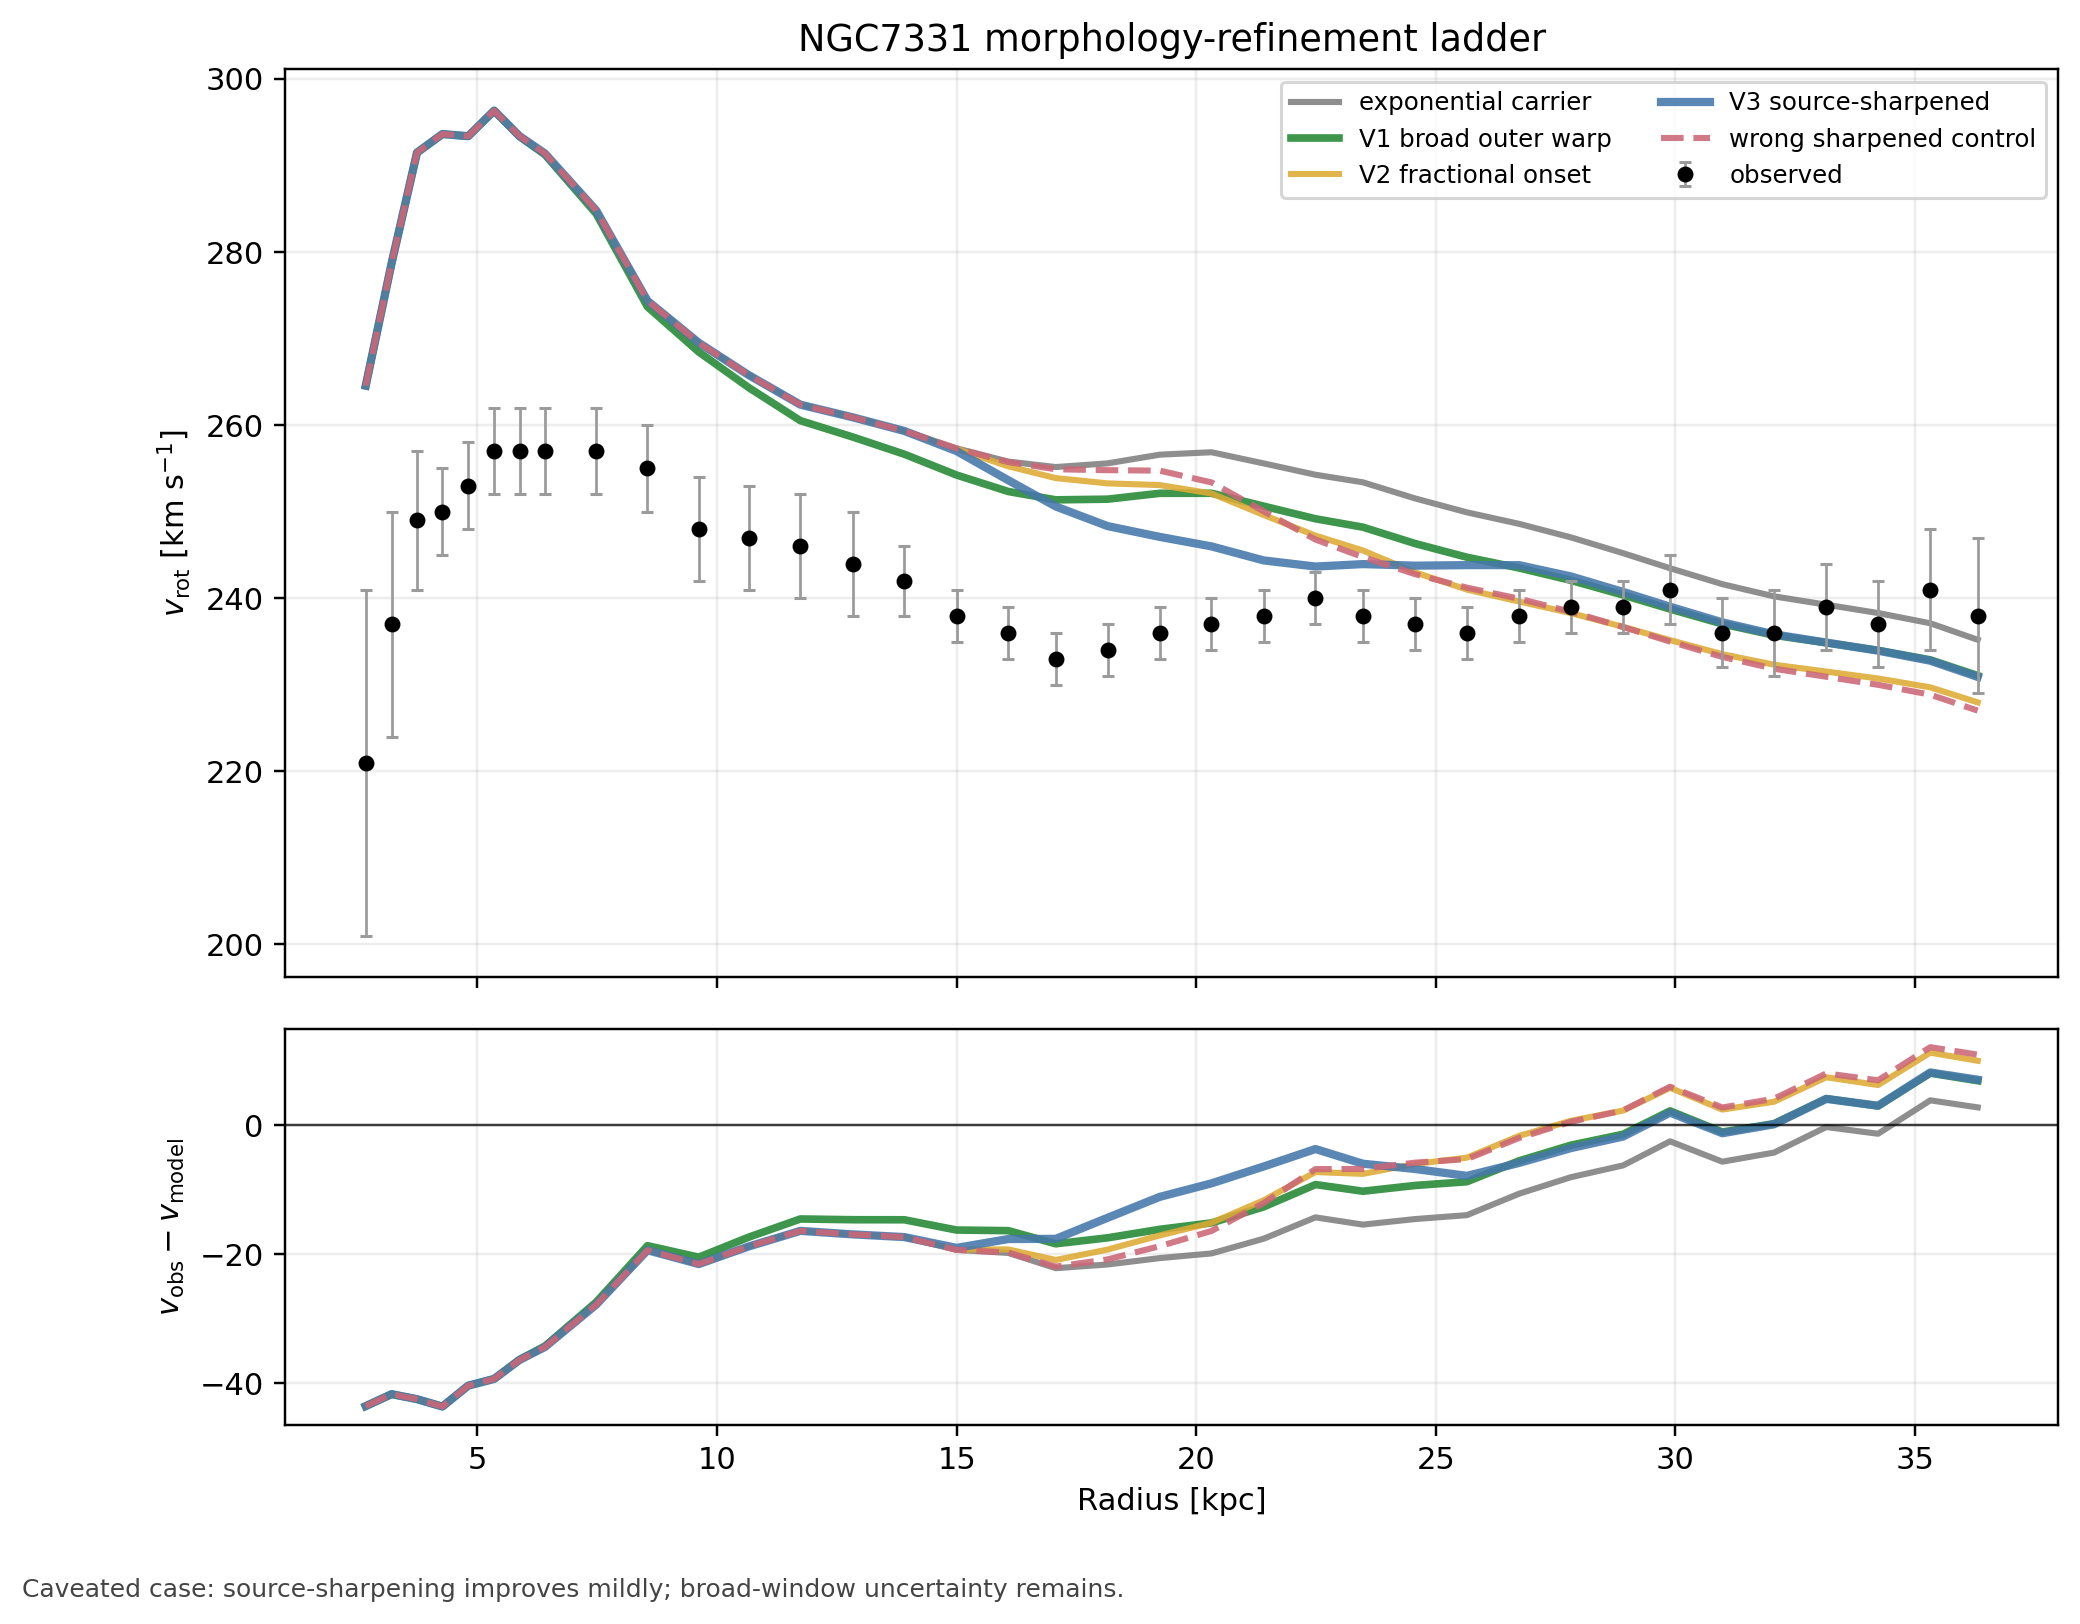
\includegraphics[width=\linewidth]{figures/fig_ngc7331_morphology_refinement_source_sharpening.png}
\caption{NGC7331 source-sharpening replay.  The broad outer-warp window gives
a modest gain over the exponential carrier, while the source-sharpened replay
is slightly better and the wrong-projection sharpened control is worse.  The
case remains caveated because the accepted route still depends on a broad
vertical/outer-warp window.}
\label{fig:ngc7331-morphology-refinement-source-sharpening}
\end{figure}

Together these refinement ladders clarify the paper's intended empirical
logic.  A more detailed morphology description is allowed to improve the
readout only when it is frozen from source-side information before scoring.
When the extra layer merely overlaps an already-used source channel, the
protocol keeps it as a control even if its RMSE happens to improve.  The
scientific signal is therefore not ``add more terms until the curve follows
the data'', but ``source-complete morphology selects a more appropriate
readout family, and inappropriate extra channels are preserved as controls''.

\subsection{Morphology adequacy review for NGC4088 and NGC4013}
\label{subsec:ngc4088-ngc4013-morphology-adequacy}

Because NGC4088 and NGC4013 carry much of the visible refinement narrative,
we also record a separate source-side morphology adequacy review.  This review
does not read endpoint residuals.  It asks only whether the assigned
readout-relevant morphology is source-supported and whether it is precise
enough for the role claimed in this paper.  The full ledger is released as
\texttt{ngc4088\_ngc4013\_morphology\_adequacy\_review\_*} under
\texttt{data/derived/}, with the markdown report under \texttt{reports/}.

\begin{description}
\item[NGC4088.]
The \(K_{\rm warp/history}\) direction is source-supported.  The distorted,
asymmetric warped H~I disk and companion/history context strongly support the
warp/history classification, so the family is not being inferred from the
rotation residual.  However, the numeric morphology precision is still open:
independent acceptance of \(x_{\rm warp}\), \(q_{\rm warp}\), memory/history,
and the \(\epsilon_{\rm cross}\) bound is required before this becomes a
source-complete endpoint-grade morphology label.

\item[NGC4013.]
The mixed exponential-disk plus warp/vertical-overlay direction is source
supported at caveated prospective-protocol level.  The compact lane is
source-rejected, while smooth edge-disk, warp/flare, vertical component, and
lag-context evidence support the mixed-overlay classification.  The result is
not retroactive validation, and the \(\Xi_t\) overlay remains a double-counting
control under the source-token priority protocol unless new non-overlap
evidence is supplied.
\end{description}

In both rows the adequacy review uses source ledgers only and explicitly
forbids observed-velocity or residual inputs.  Its function is to prevent the
paper from treating curve improvement itself as morphology evidence.

A follow-up source-strengthening packet sharpens this verdict.  For NGC4088,
Verheijen and Sancisi's H~I atlas directly supports a strongly distorted disk,
a strong position--velocity asymmetry, an asymmetric warp, side-dependent
position-angle change, and nearby companion/history context
\cite{VerheijenSancisi2001UrsaMajorHI}.  This upgrades the broad
warp/history class to strong qualitative source support, but it still does not
accept the numeric \(x_{\rm warp}\), \(q_{\rm warp}\), memory/history, or
\(\epsilon_{\rm cross}\) fields.  For NGC4013, the source situation is more
numeric: the H~I modelling gives a line-of-sight warp onset near
\(1.2'\simeq 10\) kpc, a warp orientation of about \(70^\circ\) from the line
of sight, model scale heights of 500, 350, and 210 pc across the one-component,
warp, and warp-plus-flare models, and a lag that shallows from
\(-35\) km\,s\(^{-1}\) kpc\(^{-1}\) at 5.8 kpc to zero near \(R_{25}\)
\cite{ZschaechnerRand2015NGC4013HI}.  The Spitzer vertical decomposition also
supports an extra flattened component with \(z_{\rm EC}\sim 3\) kpc and
roughly 20--26 per cent of the disk mass
\cite{Comeron2011NGC4013Vertical}.  Thus NGC4013 is strengthened at
source-numeric mixed-overlay level, while NGC4088 is strengthened at broad
class level only.  The corresponding packet is
\texttt{ngc4088\_ngc4013\_strengthened\_source\_review\_*} under
\texttt{data/derived/}.

We therefore reran a separate score-consequence audit with the source review
held fixed.  For NGC4013, the source-supported refinement gives the expected
directional improvement: the original compact proxy has RMSE \(16.99\)
km\,s\(^{-1}\), the warp/vertical-overlay route has \(11.45\)
km\,s\(^{-1}\), and the prospective exponential-disk plus WVO frozen protocol
has \(10.61\) km\,s\(^{-1}\).  The last number is the strongest NGC4013 score
in this packet, but it remains prospective/protocol-only rather than
retroactive endpoint validation.  For NGC4088, the accepted warp/history route
already has RMSE \(11.62\) km\,s\(^{-1}\), beating the best local baseline
\((25.40\) km\,s\(^{-1})\) and all wrong-family controls.  The additive,
clock-only, and additive-plus-clock control replays can reach \(9.39\),
\(10.50\), and \(8.38\) km\,s\(^{-1}\), respectively, but those improvements
remain controls because the source-strengthening packet has not promoted new
endpoint-grade \(x_{\rm warp}\), \(q_{\rm warp}\), memory/history, or
\(\epsilon_{\rm cross}\) inputs that survive the
Subsection~\ref{subsec:source-token-priority} \(T/A\) test.  The score ledger is released as
\texttt{ngc4088\_ngc4013\_strengthened\_scoring\_audit\_*}.

\begin{figure}[H]
\centering
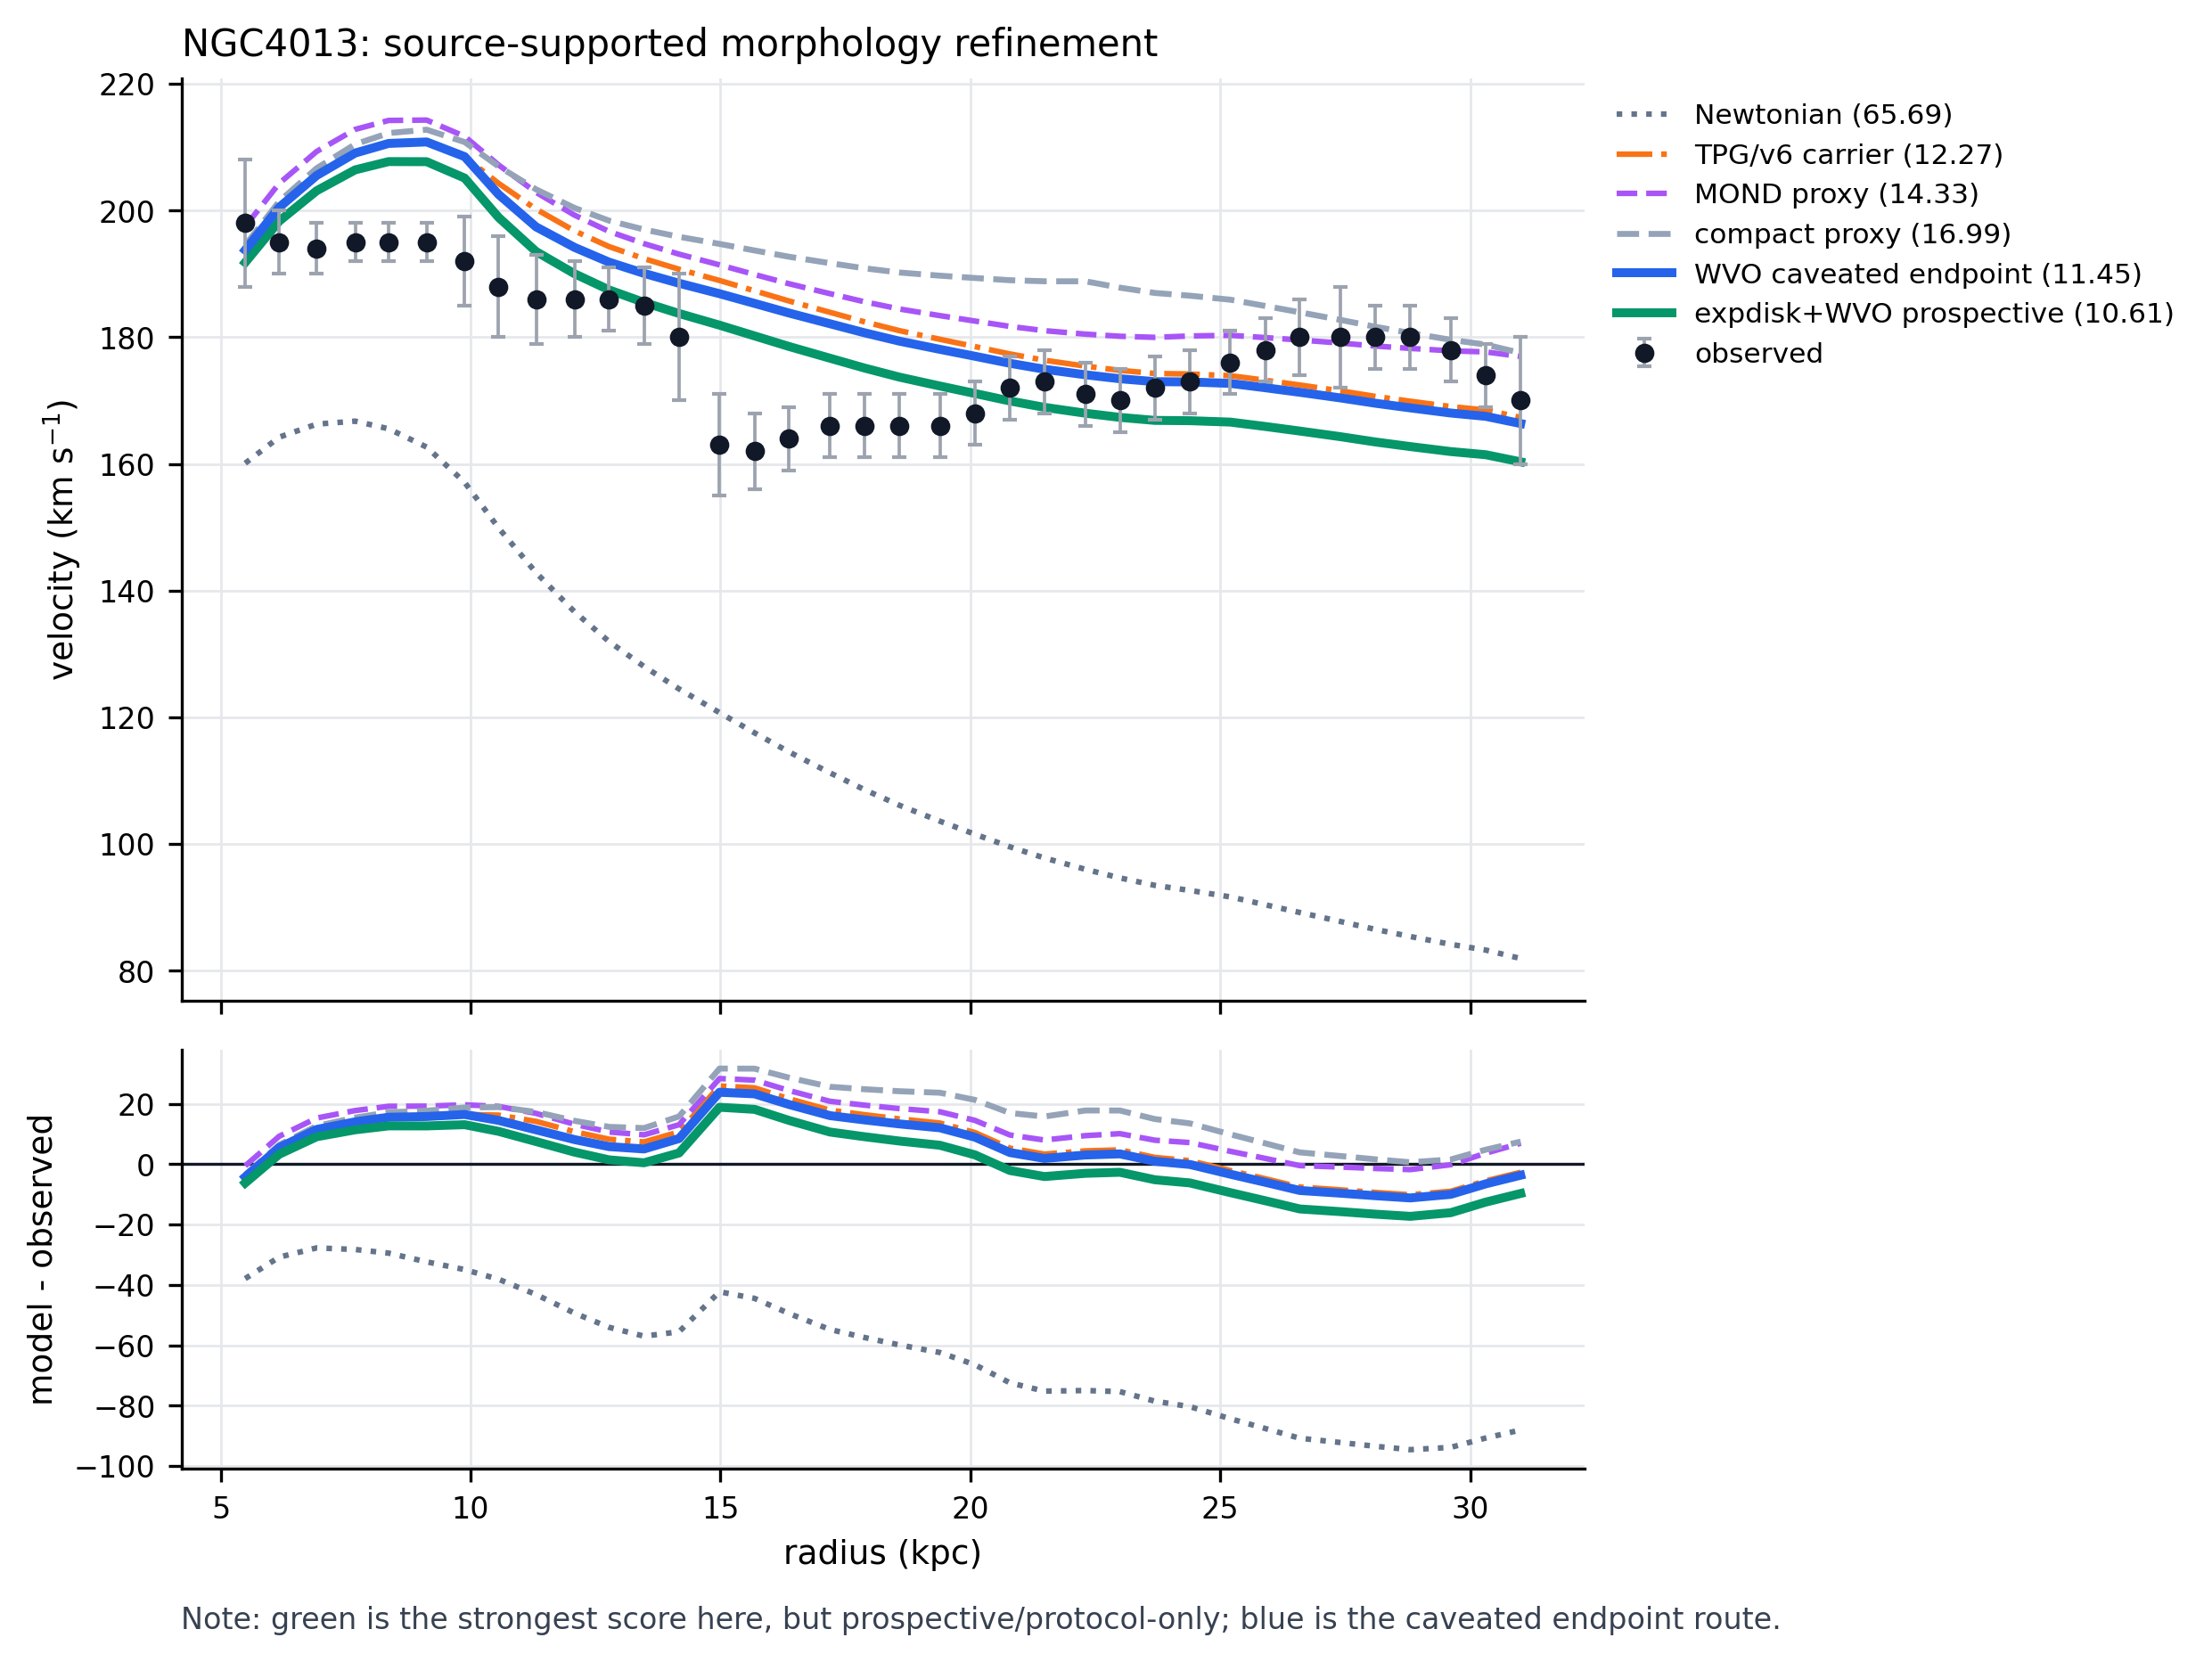
\includegraphics[width=\linewidth]{figures/fig_ngc4013_strengthened_rotation_comparison.png}
\caption{NGC4013 strengthened rotation comparison.  The source-rejected
compact proxy is shown against the source-supported warp/vertical-overlay
route, the prospective exponential-disk plus WVO protocol, and the local
Newtonian, TPG/v6, and MOND comparators.  The green curve gives the lowest
RMSE in this packet, but remains prospective/protocol-only; the blue curve is
the caveated endpoint route.}
\label{fig:ngc4013-strengthened-rotation-comparison}
\end{figure}

\begin{figure}[H]
\centering
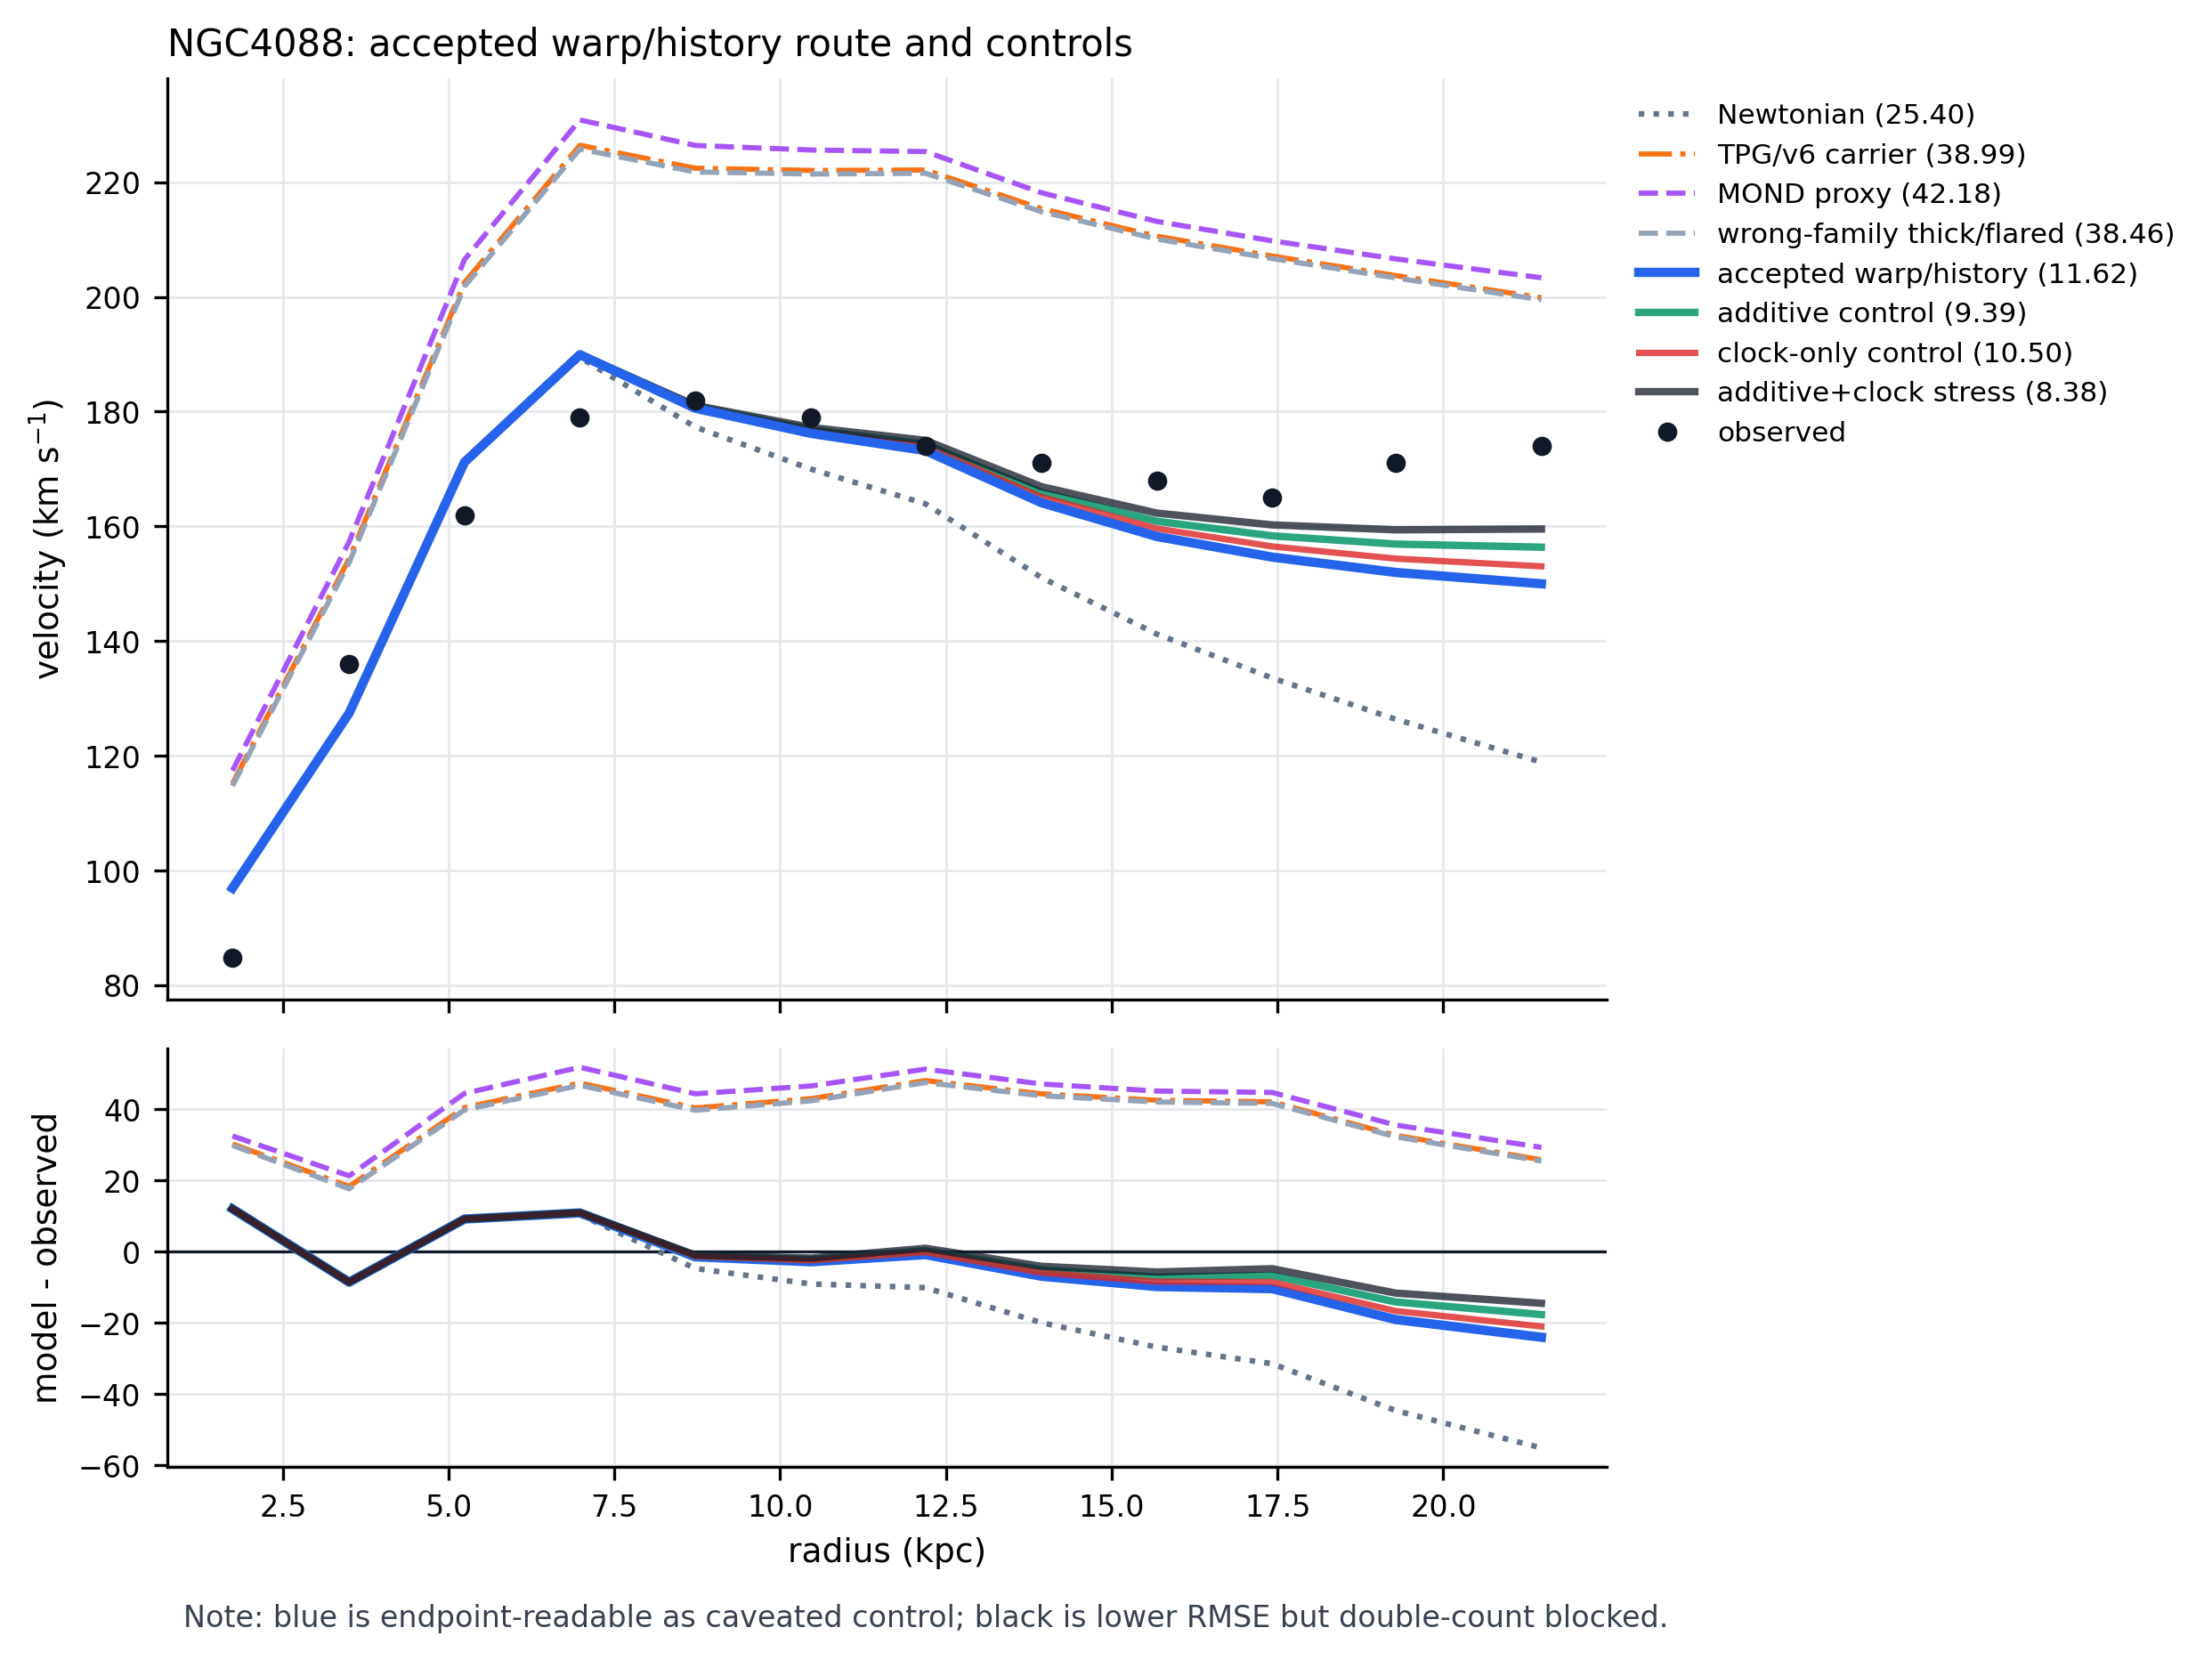
\includegraphics[width=\linewidth]{figures/fig_ngc4088_strengthened_rotation_comparison.png}
\caption{NGC4088 strengthened rotation comparison.  The accepted warp/history
route is compared with Newtonian, TPG/v6, MOND, a wrong-family thick/flared
control, and additive/time projection controls.  The black stress curve has
the lowest RMSE, but remains double-count blocked; the blue warp/history route
is the endpoint-readable caveated control.}
\label{fig:ngc4088-strengthened-rotation-comparison}
\end{figure}

The double-count statement for NGC4088 is not only a verbal caveat.  We also
release an explicit non-overlap certificate implementing the source-token
priority protocol of Subsection~\ref{subsec:source-token-priority}.  Let \(A\) denote the source
subspace already assigned to the accepted additive warp/history route, generated
by warp geometry, radial onset, \(q_{\rm warp}\) source strength, and
morphology-history phase.  Let \(T\) denote the current \(\Xi_t\) source ledger.
The ledger contains four terms: \(f_{\rm PA}\), \(f_R\), \(f_q\), and
\(f_{\rm mem}\).  The certificate maps these respectively to shared warp
geometry, shared radial-onset support, direct \(q_{\rm warp}\) source-strength
overlap, and shared morphology-history phase.  Hence all current \(\Xi_t\)
generators lie in \(A\), and the endpoint-admissible clock load is the quotient
load in \(T/A\).  Numerically the raw clock load is \(1.375\), but the
orthogonal load is zero.  Therefore the accepted combined route must set
\(\Xi_{\rm eff}=1\), and the lower-RMSE additive-plus-clock curve remains a
stress/control curve rather than endpoint evidence.  The certificate is
released as
\texttt{ngc4088\_time\_projection\_nonoverlap\_certificate\_*}.

\begin{landscape}
\section{Per-kernel derivation ledger}
\label{sec:per-kernel-derivation-ledger}

Table~\ref{tab:per-kernel-derivation-ledger} makes explicit how the main
kernels used in this paper are obtained.  The point of the table is not to add
new results; it is to expose the derivation chain that is otherwise spread
across source-review, formula-freeze, and scoring artifacts.  A row is
endpoint-readable only when the source label, radial support, amplitude or
carrier rule, and non-overlap status are all frozen before scoring.  Otherwise
the row is retained as a control, diagnostic, candidate, or blocked route.
Endpoint-readable also remains weaker than source-grounded: rows in this ledger
are operational kernels unless a separate projection-induction derivation
establishes the Tau-side activation, quotient survival, closure stability, and
4D readout survival of the channel.

\begingroup
\scriptsize
\setlength{\tabcolsep}{2pt}
\begin{longtable}{@{}p{0.13\linewidth}p{0.18\linewidth}p{0.19\linewidth}p{0.23\linewidth}p{0.18\linewidth}@{}}
\caption{Per-kernel derivation ledger for the concrete readout families used
or proposed in Paper~2.  ``Formula role'' gives the operational kernel shell,
not a validated universal law.  ``Status'' records the claim boundary used in
the paper.}
\label{tab:per-kernel-derivation-ledger}\\
\toprule
Kernel route & Source statement & Observable / frozen input & Formula role & Status / artifact family \\
\midrule
\endfirsthead
\toprule
Kernel route & Source statement & Observable / frozen input & Formula role & Status / artifact family \\
\midrule
\endhead
\bottomrule
\endfoot

Morphology-only family &
Residual-blind projected morphology class such as scale-tail, compact,
exponential, ring, or thick/flared disk &
Accepted morphology label and class-specific radial support proxy &
\(\delta v_K^2=A_KK_K(R)\) &
preflight baseline family; upgraded only when source manifest and amplitude
freeze pass \\

Projection-enriched mixed family &
Present morphology alone is insufficient because observer/path visibility,
warp, flare, vertical overlay, or trajectory phase changes the effective readout &
Channel components \(K_j(R)\), visibility weights \(w_j(R)\), and source-side
amplitudes \(A_j\) &
\(\delta v_{\rm proj}^2=\sum_j A_jw_jK_j\) &
general Paper~2 shell; requires source-token and non-overlap gates \\

NGC4013 warp/vertical overlay &
Smooth edge-on disk plus warp/flare, vertical component, and lag context &
Warp onset near \(1.2'\), warp orientation, scale-height models, lag profile,
and Spitzer extra component &
mixed warp/vertical-overlay radial gate added to an exponential-disk carrier &
caveated endpoint/protocol route; \(\Xi_t\) overlay is a double-counting control \\

NGC4088 warp/history &
Distorted, asymmetric warped H~I disk with companion/history context &
Broad warp/history support, side-dependent position-angle change, asymmetric
H~I morphology, and memory/history proxy &
additive warp/history morphology route with \(\Xi_{\rm eff}=1\) after
non-overlap audit &
caveated accepted control route; additive-plus-clock remains stress/control
because \(T/A=0\) \\

NGC7331 outer-warp sharpening &
Projected disk with caveated vertical/outer-warp structure &
Broad outer-warp window and source-sharpened radial onset controls &
outer-warp / vertical support window applied to projected-disk carrier &
caveated source-sharpening route; not a final source-complete endpoint \\

NGC5907 edge-on projection &
Highly edge-on projected disk where observer/path projection is already strong &
Edge-on geometry, warp/truncation context, and projection saturation flag &
projection-saturated mixed kernel; richer path term only if new source data
justify it &
near-neutral/saturated control; no active extra channel without new evidence \\

NGC0891 / NGC4217 EVH--DVH &
Pure global beta transfer overshoots; source review supports edge-on
vertical/dust/H~I/radio-halo readout &
Edge-on dust lanes, H~I halo, extra-planar gas, radio/halo evidence, and disk
scale \(R_s\) &
\(v^2=v_{\rm carrier}^2[1+(\beta_{\rm cl}-1)K_{\rm EVH/DVH}(R)]\) &
source-blind morphology-refinement controls; ordered improvement, not
population validation \\

UGC12506 \(\Theta_{\rm morph}\) &
Late-settling / projection-history morphology phase is plausible but not
sufficient as a clock endpoint &
Outer radial shape and source-status load assigned to morphology-state phase &
\(v_\theta^2=v_{\rm projection/history}^2+A_\theta K_\theta(R)\) &
diagnostic/control; improves directionally but remains non-endpoint \\

UGC12506 \(\Xi_t\) interval &
High-inclination, high-spin, extended H~I envelope suggests a small
clock/readout interval, with path term set to zero &
Source load \(L\), protocol cap \(\epsilon_{\rm cap}=0.035\), and frozen
\(\epsilon_t\) interval &
\(\Xi_t(R)=1+\epsilon_tK_t(R)\), with
\(\epsilon_t=\epsilon_{\rm cap}L/(1+L)\) &
caveated interval/control manifest; endpoint blocked until \(K_t\) and cap
origin are accepted \\

UGC12506 mass/envelope closure &
Source-native NFW/high-spin envelope route has good shape but missing
normalization &
Spin proxy, NFW/HSE preference, inclination, and selected carrier route &
\(v^2=\beta_{\rm cl}v_{\rm carrier}^2\), with \(\beta_{\rm cl}\) source-derived
but post-diagnostic in this draft &
strong post-diagnostic source candidate; requires independent transfer before
endpoint use \\

IC4202 smooth-disk projection prekernel &
Fresh projection-rich smooth edge-on candidate has a source-supported active
branch but missing value freeze &
Inclination and disk support window \(W_{\rm disk}(R;R_s,R_{\rm HI})\) &
\(K_{\rm pre}(R)=\sin^2i\,W_{\rm disk}(R;R_s,R_{\rm HI})\) &
formula/kernel blocked; needs \(q_{\rm reg}\), \(z_{\rm cl}\), and
\(e_{\rm proj}\) freeze \\

\end{longtable}
\endgroup
\end{landscape}

This ledger is deliberately asymmetric: some rows are formula shells, some are
control kernels, and some are blocked future routes.  That asymmetry is a
feature of the protocol.  The paper does not claim that every listed kernel is
validated.  It claims that when a kernel is used, the path from source
morphology to radial formula, amplitude/carrier rule, and endpoint status is
auditable.

\section{Problematic-case route ledger}
\label{sec:problematic-ledger}

\subsection{Candidate projection channels for problematic cases}

The same audit also tells us which additional projection channels are worth
trying next, and which ones should remain inactive.  Table~\ref{tab:problematic-channel-ledger}
is a route ledger, not a score table.  It records the most plausible
Tau-morphology-state projection channel for each problematic or caveated
galaxy, together with the immediate guardrail.  No row in the table authorizes
an endpoint score by itself.

\begin{table}[H]
\centering
\scriptsize
\setlength{\tabcolsep}{2pt}
\begin{tabularx}{\linewidth}{@{}l p{0.23\linewidth} p{0.24\linewidth} X@{}}
\toprule
Galaxy & Current role & Priority channel & Required next gate \\
\midrule
UGC12506 &
primary stress case, still underpredicted &
mass/envelope plus metric-closure readout; observer/path and clock remain
secondary controls &
derive a source-frozen mass/envelope--closure kernel and ablate it against the
\(\Theta_{\rm morph}\) and \(\Xi_t\)-cap controls \\
NGC4088 &
improving warp/history/asymmetry case &
trajectory/phase and asymmetry/history readout; clock only as control &
keep the accepted additive warp/history route with \(\Xi_{\rm eff}=1\);
reopen clock only with non-overlapping evidence that survives the \(T/A\)
source-token priority test \\
NGC4013 &
worsened mixed-overlay case &
mixed warp/vertical-overlay readout; no current \(\Xi_t\) promotion &
preserve as a retrospective mixed-reference control unless a fresh analogue or
independent clock observable is found \\
NGC7331 &
worsened broad outer-warp case &
sharpened vertical/outer-warp readout; metric/closure only after window
sharpening &
freeze a narrower outer-warp/vertical window before adding any clock or
closure layer \\
NGC5907 &
near-neutral projection-saturated case &
observer/path edge-on projection and warp/truncation &
treat as projection-saturated unless new path or vertical profile data justify
a richer channel \\
NGC4183 &
weak/null projection control &
quiet weak-projection limit &
retain as null control; do not introduce active projection channels without
new source evidence \\
\bottomrule
\end{tabularx}
\caption{Candidate projection-channel ledger for problematic and caveated
galaxies.  The table records the next plausible source-side readout channel,
not an endpoint promotion.  Every listed new channel remains gated by
source-freeze, non-overlap, and ablation tests before scoring.}
\label{tab:problematic-channel-ledger}
\end{table}

We also convert this ledger into an executable next-gate CSV artifact.  The
artifact is explicitly marked as a not-endpoint gate plan; it contains six
galaxies and authorizes zero endpoint promotions.  Two rows
have control/replay paths: UGC12506 proceeds only to a source-native
NFW/HSE mass-envelope plus metric-closure ablation against the
\(\Theta_{\rm morph}\)-only, \(\Theta_{\rm morph}+\Xi_t\)-cap, and
source-envelope controls; NGC4088 keeps the accepted additive warp/history
route while clock readout remains a control.  The other rows stay inactive or
blocked: the current NGC4013 \(\Xi_t\) proxy is rejected as double-counting,
NGC7331 needs source-sharpened outer-warp/vertical windowing before refined
replay, NGC5907 is projection-saturated at the current proxy level, and NGC4183
remains the weak/null projection control.

\section{Predeclared projection-enriched population-validation gate}
\label{sec:population-gate}

The current audit motivates a catalogue test but does not pass one.  A
population claim requires a residual-blind projection-enriched catalogue in
which source-frozen observer/projection labels select the enriched family before
endpoint scoring.  The released protocol artifacts define the next endpoints:
\begin{description}[leftmargin=*]
  \item[\texttt{DELTA\_ENRICHED\_SIMPLER}] enriched matched RMSE versus the
  simpler morphology-only proxy;
  \item[\texttt{DELTA\_ENRICHED\_WRONG}] enriched matched RMSE versus wrong
  projection-enriched families;
  \item[\texttt{SHUFFLED\_PROJECTION\_LABEL\_NULL}] matched enriched score
  versus shuffled observer/projection labels;
  \item[\texttt{BASELINE\_COMPETITIVENESS}] enriched matched readout versus
  Newtonian, MOND/RAR-like, TPG/v6-like, and RMOND-facing comparators;
  \item[\texttt{TRAJECTORY\_PHASE\_ABLATION}] present-only, trajectory-enriched,
  and trajectory/phase-enriched morphology kernels compared as a staged
  ablation;
  \item[\texttt{PATH\_ENVIRONMENT\_ABLATION}] source-only, source-plus-observer,
  and path-environment kernels compared as a staged ablation.
\end{description}

The present status is the blocked gate
\begin{center}
\small
\begin{tabular}{c}
\texttt{PROJECTION\_ENRICHED\_POPULATION\_VALIDATION\_BLOCKED}\\
\texttt{CATALOGUE\_AND\_WRONG\_LABEL\_GATES}.
\end{tabular}
\end{center}
The gate requires at least 12 source-rich catalogue cases and at least 8 fresh
cases not used in the current candidate audit.  Endpoint scores are not run
in this manuscript.  Diagnostic scores are not allowed as label inputs.

\section{Catalogue expansion status}
\label{sec:catalogue-expansion}

The population gate is blocked, but not empty.  The current expansion ledger
contains 18 projection-rich rows: the five inspected candidate cases, one
weak/null projection control, one frozen-protocol transfer seed, one
formula-blocked named candidate, and 10 additional fresh projection-catalogue
queue objects selected from residual-blind orientation/projection manifests.
Twelve rows are potential fresh catalogue cases, satisfying the numerical size
target in principle, but they are not formula-frozen endpoint cases.

\begin{table}[H]
\centering
\small
\begin{tabularx}{\linewidth}{lrrX}
\toprule
Quantity & Current & Required & Interpretation \\
\midrule
Catalogue rows listed & 18 & 12 & enough rows to define an expansion queue \\
Fresh candidate rows & 12 & 8 & enough possible fresh cases in principle \\
Formula/kernel blocked rows & 12 & 0 & population validation remains blocked \\
Source/orientation blocked rows & 12 & 0 & source-side catalogue work is the main bottleneck \\
Wrong-label caveated seed rows & 2 & 0 & NGC5907 and NGC7331 need replay controls \\
\bottomrule
\end{tabularx}
\caption{Projection-enriched population expansion status.  These counts come
from the expansion ledger and are preparation counts, not endpoint scores.}
\label{tab:projection-expansion-status}
\end{table}

NGC3198 is now a useful transfer seed rather than a population-validation row:
a source-derived constant-\(H\) HALOGAS/EPG frozen protocol has been scored, but
the same galaxy was already diagnostically inspected, so it cannot be counted as
a fresh endpoint validation.  IC4202 is the most concrete formula-blocked fresh
candidate: it has an edge-on smooth-disk projection shell, but the
projection-load values and closure normalization are not yet frozen.  The
broader queue contains high-inclination or projection-ready SPARC objects such
as UGC07151, UGCA444, IC2574, and UGC06818, but these still need
source-native orientation promotion, morphology-trajectory acceptance, and
formula freeze manifests before scoring.

The IC4202 blocker has now been reduced to a value-freeze obligation rather
than a generic morphology uncertainty.  A source-supported projection prekernel
\(K_{\rm pre}(R)=\sin^2 i\,W_{\rm disk}(R;R_s,R_{\rm HI})\) is available from
residual-blind support and inclination data.  The nonzero active branch remains
blocked only because \(q_{\rm reg}(R)\), \(z_{\rm cl}(R)\), and the independent
projection/load scalar \(e_{\rm proj}\) are not source-frozen.  Acceptable
resolutions are a source-native H\,I regularity/closure profile or a
Tau-side value theorem fixed before endpoint scoring.  Reusing inclination as
the independent projection load, or using the observed rotation residual to set
these values, is explicitly forbidden.

Thus the next validation step is concrete: resolve at least eight fresh source,
orientation, and trajectory-phase blockers; build formula-freeze manifests; and
then run the matched-versus-simpler, wrong-enriched, shuffled projection-label,
trajectory-phase ablation, and baseline endpoints.  Until those gates pass, the
correct status remains catalogue expansion, not population validation.

\section{Conclusion}

Projection-enriched kernels are the natural next step after morphology-only
forward readouts.  The inspected galaxies show that adding observer/projection
and morphology-trajectory information can improve the matched kernel over a
simpler one-dimensional proxy, sometimes enough to cross a practical baseline
competitiveness threshold.  UGC12506 is deliberately retained as a cautionary
case: projection-history enrichment improves the Tau curve substantially
relative to simpler source shells, but still does not reach the strongest
listed MOND/TPG diagnostic curves.  The reason this case improves is also
physically interpretable inside the source ledger: high inclination, high spin,
an extended H~I envelope, and projection-history stress all point toward a
non-negligible observer/projection and clock-readout correction.  This supports
kernel development, not population validation.  The full-time morphology phase
replay adds an
important negative-control feature: the extra trajectory/phase layer is not a
universal gain term.  It improves the strongest warp/history/asymmetry case
(NGC4088), where the source-side morphology already indicates an unsettled
warp/history/asymmetry state; it is nearly neutral in the weak or already
saturated projection cases, and slightly worsens two already close
mixed/projection kernels.  This pattern is consistent with a
morphology/history-dependent time/projection readout correction rather than an
unconstrained curve-fitting knob.

The same pattern enforces the source-coordinate non-double-counting rule.  A
time/projection factor is not accepted merely because it improves a curve.  It
must either have source support independent of the active morphology/projection
kernel, or be represented as a shared quotient contribution.  When the support
ledger overlaps, the extra factor remains a diagnostic/control curve even if it
lowers RMSE.

The next scientific step is a predeclared projection-enriched catalogue test:
source-frozen observer/projection labels must select enriched kernels before
endpoint scoring, trajectory/phase proxies must be frozen from source-side
evidence before use, wrong enriched families and shuffled projection labels
must be run as controls, and baseline comparisons must be reported without
universal superiority claims unless the population endpoint actually passes.
The expansion ledger shows that a plausible candidate queue exists, but source
and formula-freeze blockers remain.  Any channel promoted beyond control or
proxy status must also pass the source-grounding gate: activation, quotient
survival, closure stability, and 4D readout survival.  A still fuller
path-aware kernel requires source-observer light-bundle and metric-environment
data that are not yet modeled here.

The paper therefore establishes three limited results.  First,
projection-enriched and time-readout layers can be made testable as
source-frozen controls rather than residual-fitted corrections.  Second, the
current controls are selective: they improve disturbed or projection-rich cases
but remain neutral or worsen in already saturated systems, which argues against
a universal gain-knob interpretation.  Third, the beta-closure expression is a
transfer hypothesis generated by the UGC12506 stress test, not same-galaxy
validation.  Its evidential test is independent, predeclared transfer to other
high-spin edge-on systems.

Within the wider Tau Core programme, this result is best read as support for a
multi-scale readout architecture rather than as a direct quantum or gravity
recovery claim.  The same deeper projection-state vocabulary may later connect
galaxy, lensing, cosmology, and quantum/coherence channels, but the present
paper validates only the source-frozen projection-readout protocol described
above.

\bibliographystyle{plain}
\bibliography{refs}

\end{document}
